% Options for packages loaded elsewhere
\PassOptionsToPackage{unicode}{hyperref}
\PassOptionsToPackage{hyphens}{url}
\PassOptionsToPackage{dvipsnames,svgnames,x11names}{xcolor}
%
\documentclass[
  letterpaper,
  DIV=11,
  numbers=noendperiod]{scrreprt}

\usepackage{amsmath,amssymb}
\usepackage{iftex}
\ifPDFTeX
  \usepackage[T1]{fontenc}
  \usepackage[utf8]{inputenc}
  \usepackage{textcomp} % provide euro and other symbols
\else % if luatex or xetex
  \usepackage{unicode-math}
  \defaultfontfeatures{Scale=MatchLowercase}
  \defaultfontfeatures[\rmfamily]{Ligatures=TeX,Scale=1}
\fi
\usepackage{lmodern}
\ifPDFTeX\else  
    % xetex/luatex font selection
\fi
% Use upquote if available, for straight quotes in verbatim environments
\IfFileExists{upquote.sty}{\usepackage{upquote}}{}
\IfFileExists{microtype.sty}{% use microtype if available
  \usepackage[]{microtype}
  \UseMicrotypeSet[protrusion]{basicmath} % disable protrusion for tt fonts
}{}
\makeatletter
\@ifundefined{KOMAClassName}{% if non-KOMA class
  \IfFileExists{parskip.sty}{%
    \usepackage{parskip}
  }{% else
    \setlength{\parindent}{0pt}
    \setlength{\parskip}{6pt plus 2pt minus 1pt}}
}{% if KOMA class
  \KOMAoptions{parskip=half}}
\makeatother
\usepackage{xcolor}
\setlength{\emergencystretch}{3em} % prevent overfull lines
\setcounter{secnumdepth}{5}
% Make \paragraph and \subparagraph free-standing
\ifx\paragraph\undefined\else
  \let\oldparagraph\paragraph
  \renewcommand{\paragraph}[1]{\oldparagraph{#1}\mbox{}}
\fi
\ifx\subparagraph\undefined\else
  \let\oldsubparagraph\subparagraph
  \renewcommand{\subparagraph}[1]{\oldsubparagraph{#1}\mbox{}}
\fi

\usepackage{color}
\usepackage{fancyvrb}
\newcommand{\VerbBar}{|}
\newcommand{\VERB}{\Verb[commandchars=\\\{\}]}
\DefineVerbatimEnvironment{Highlighting}{Verbatim}{commandchars=\\\{\}}
% Add ',fontsize=\small' for more characters per line
\usepackage{framed}
\definecolor{shadecolor}{RGB}{241,243,245}
\newenvironment{Shaded}{\begin{snugshade}}{\end{snugshade}}
\newcommand{\AlertTok}[1]{\textcolor[rgb]{0.68,0.00,0.00}{#1}}
\newcommand{\AnnotationTok}[1]{\textcolor[rgb]{0.37,0.37,0.37}{#1}}
\newcommand{\AttributeTok}[1]{\textcolor[rgb]{0.40,0.45,0.13}{#1}}
\newcommand{\BaseNTok}[1]{\textcolor[rgb]{0.68,0.00,0.00}{#1}}
\newcommand{\BuiltInTok}[1]{\textcolor[rgb]{0.00,0.23,0.31}{#1}}
\newcommand{\CharTok}[1]{\textcolor[rgb]{0.13,0.47,0.30}{#1}}
\newcommand{\CommentTok}[1]{\textcolor[rgb]{0.37,0.37,0.37}{#1}}
\newcommand{\CommentVarTok}[1]{\textcolor[rgb]{0.37,0.37,0.37}{\textit{#1}}}
\newcommand{\ConstantTok}[1]{\textcolor[rgb]{0.56,0.35,0.01}{#1}}
\newcommand{\ControlFlowTok}[1]{\textcolor[rgb]{0.00,0.23,0.31}{#1}}
\newcommand{\DataTypeTok}[1]{\textcolor[rgb]{0.68,0.00,0.00}{#1}}
\newcommand{\DecValTok}[1]{\textcolor[rgb]{0.68,0.00,0.00}{#1}}
\newcommand{\DocumentationTok}[1]{\textcolor[rgb]{0.37,0.37,0.37}{\textit{#1}}}
\newcommand{\ErrorTok}[1]{\textcolor[rgb]{0.68,0.00,0.00}{#1}}
\newcommand{\ExtensionTok}[1]{\textcolor[rgb]{0.00,0.23,0.31}{#1}}
\newcommand{\FloatTok}[1]{\textcolor[rgb]{0.68,0.00,0.00}{#1}}
\newcommand{\FunctionTok}[1]{\textcolor[rgb]{0.28,0.35,0.67}{#1}}
\newcommand{\ImportTok}[1]{\textcolor[rgb]{0.00,0.46,0.62}{#1}}
\newcommand{\InformationTok}[1]{\textcolor[rgb]{0.37,0.37,0.37}{#1}}
\newcommand{\KeywordTok}[1]{\textcolor[rgb]{0.00,0.23,0.31}{#1}}
\newcommand{\NormalTok}[1]{\textcolor[rgb]{0.00,0.23,0.31}{#1}}
\newcommand{\OperatorTok}[1]{\textcolor[rgb]{0.37,0.37,0.37}{#1}}
\newcommand{\OtherTok}[1]{\textcolor[rgb]{0.00,0.23,0.31}{#1}}
\newcommand{\PreprocessorTok}[1]{\textcolor[rgb]{0.68,0.00,0.00}{#1}}
\newcommand{\RegionMarkerTok}[1]{\textcolor[rgb]{0.00,0.23,0.31}{#1}}
\newcommand{\SpecialCharTok}[1]{\textcolor[rgb]{0.37,0.37,0.37}{#1}}
\newcommand{\SpecialStringTok}[1]{\textcolor[rgb]{0.13,0.47,0.30}{#1}}
\newcommand{\StringTok}[1]{\textcolor[rgb]{0.13,0.47,0.30}{#1}}
\newcommand{\VariableTok}[1]{\textcolor[rgb]{0.07,0.07,0.07}{#1}}
\newcommand{\VerbatimStringTok}[1]{\textcolor[rgb]{0.13,0.47,0.30}{#1}}
\newcommand{\WarningTok}[1]{\textcolor[rgb]{0.37,0.37,0.37}{\textit{#1}}}

\providecommand{\tightlist}{%
  \setlength{\itemsep}{0pt}\setlength{\parskip}{0pt}}\usepackage{longtable,booktabs,array}
\usepackage{calc} % for calculating minipage widths
% Correct order of tables after \paragraph or \subparagraph
\usepackage{etoolbox}
\makeatletter
\patchcmd\longtable{\par}{\if@noskipsec\mbox{}\fi\par}{}{}
\makeatother
% Allow footnotes in longtable head/foot
\IfFileExists{footnotehyper.sty}{\usepackage{footnotehyper}}{\usepackage{footnote}}
\makesavenoteenv{longtable}
\usepackage{graphicx}
\makeatletter
\def\maxwidth{\ifdim\Gin@nat@width>\linewidth\linewidth\else\Gin@nat@width\fi}
\def\maxheight{\ifdim\Gin@nat@height>\textheight\textheight\else\Gin@nat@height\fi}
\makeatother
% Scale images if necessary, so that they will not overflow the page
% margins by default, and it is still possible to overwrite the defaults
% using explicit options in \includegraphics[width, height, ...]{}
\setkeys{Gin}{width=\maxwidth,height=\maxheight,keepaspectratio}
% Set default figure placement to htbp
\makeatletter
\def\fps@figure{htbp}
\makeatother


% load packages
\usepackage{geometry}
\usepackage{xcolor}
\usepackage{eso-pic}
\usepackage{fancyhdr}
\usepackage{sectsty}
\usepackage{fontspec}
\usepackage{titlesec}


%% Set page size with a wider right margin
\geometry{a4paper, total={170mm,257mm}, left=15mm, top=20mm, bottom=25mm, right=25mm}

%% Let's define some colours
\definecolor{light}{HTML}{edf7fa}
\definecolor{highlight}{HTML}{2c6d7d}
\definecolor{dark}{HTML}{336882}

%% Let's add the border on the right hand side 
\AddToShipoutPicture{% 
    \AtPageLowerLeft{% 
        \put(\LenToUnit{\dimexpr\paperwidth-1.75cm},0){% 
            \color{light}\rule{3cm}{\LenToUnit\paperheight}%
          }%
     }%
     % logo
    % \AtPageLowerLeft{% start the bar at the bottom right of the page
    %     \put(\LenToUnit{\dimexpr\paperwidth-1.5cm},27.2cm){% move it to the top right
    %         \color{light}
\includegraphics[width=1.2cm]{_extensions/nrennie/PrettyPDF/logo.png}
    %       }%
    %  }%
}

%% Style the page number
\fancypagestyle{mystyle}{
  % \fancyhf{}
  % \renewcommand\headrulewidth{0pt}
  % Empty style
}

\pagestyle{mystyle}


% Center align chapter titles
\usepackage{titlesec}
\titleformat{\chapter}[display]
  {\normalfont\huge\bfseries\centering\color{dark}}{\chaptertitlename\ \thechapter}{20pt}{\Huge}


% add a border to images
% \let\originalincludegraphics\includegraphics
% \renewcommand{\includegraphics}[2][]{%
%   \fcolorbox{light}{white}{\originalincludegraphics[#1]{#2}}%
% }

\let\originalincludegraphics\includegraphics
\renewcommand{\includegraphics}[2][]{%
  \setlength{\fboxrule}{4pt} % Set border thickness to 2pt
  \fcolorbox{light}{white}{\originalincludegraphics[#1]{#2}}%
}



%% Use some custom fonts
\setsansfont{Ubuntu}[
    Path=_extensions/nrennie/PrettyPDF/Ubuntu/,
    Scale=0.9,
    Extension = .ttf,
    UprightFont=*-Regular,
    BoldFont=*-Bold,
    ItalicFont=*-Italic,
    ]

\setmainfont{Ubuntu}[
    Path=_extensions/nrennie/PrettyPDF/Ubuntu/,
    Scale=0.9,
    Extension = .ttf,
    UprightFont=*-Regular,
    BoldFont=*-Bold,
    ItalicFont=*-Italic,
    ]
\KOMAoption{captions}{tableheading}
\makeatletter
\@ifpackageloaded{tcolorbox}{}{\usepackage[skins,breakable]{tcolorbox}}
\@ifpackageloaded{fontawesome5}{}{\usepackage{fontawesome5}}
\definecolor{quarto-callout-color}{HTML}{909090}
\definecolor{quarto-callout-note-color}{HTML}{0758E5}
\definecolor{quarto-callout-important-color}{HTML}{CC1914}
\definecolor{quarto-callout-warning-color}{HTML}{EB9113}
\definecolor{quarto-callout-tip-color}{HTML}{00A047}
\definecolor{quarto-callout-caution-color}{HTML}{FC5300}
\definecolor{quarto-callout-color-frame}{HTML}{acacac}
\definecolor{quarto-callout-note-color-frame}{HTML}{4582ec}
\definecolor{quarto-callout-important-color-frame}{HTML}{d9534f}
\definecolor{quarto-callout-warning-color-frame}{HTML}{f0ad4e}
\definecolor{quarto-callout-tip-color-frame}{HTML}{02b875}
\definecolor{quarto-callout-caution-color-frame}{HTML}{fd7e14}
\makeatother
\makeatletter
\makeatother
\makeatletter
\@ifpackageloaded{bookmark}{}{\usepackage{bookmark}}
\makeatother
\makeatletter
\@ifpackageloaded{caption}{}{\usepackage{caption}}
\AtBeginDocument{%
\ifdefined\contentsname
  \renewcommand*\contentsname{Table of contents}
\else
  \newcommand\contentsname{Table of contents}
\fi
\ifdefined\listfigurename
  \renewcommand*\listfigurename{List of Figures}
\else
  \newcommand\listfigurename{List of Figures}
\fi
\ifdefined\listtablename
  \renewcommand*\listtablename{List of Tables}
\else
  \newcommand\listtablename{List of Tables}
\fi
\ifdefined\figurename
  \renewcommand*\figurename{Figure}
\else
  \newcommand\figurename{Figure}
\fi
\ifdefined\tablename
  \renewcommand*\tablename{Table}
\else
  \newcommand\tablename{Table}
\fi
}
\@ifpackageloaded{float}{}{\usepackage{float}}
\floatstyle{ruled}
\@ifundefined{c@chapter}{\newfloat{codelisting}{h}{lop}}{\newfloat{codelisting}{h}{lop}[chapter]}
\floatname{codelisting}{Listing}
\newcommand*\listoflistings{\listof{codelisting}{List of Listings}}
\makeatother
\makeatletter
\@ifpackageloaded{caption}{}{\usepackage{caption}}
\@ifpackageloaded{subcaption}{}{\usepackage{subcaption}}
\makeatother
\makeatletter
\@ifpackageloaded{tcolorbox}{}{\usepackage[skins,breakable]{tcolorbox}}
\makeatother
\makeatletter
\@ifundefined{shadecolor}{\definecolor{shadecolor}{rgb}{.97, .97, .97}}
\makeatother
\makeatletter
\@ifundefined{codebgcolor}{\definecolor{codebgcolor}{named}{light}}
\makeatother
\makeatletter
\makeatother
\ifLuaTeX
  \usepackage{selnolig}  % disable illegal ligatures
\fi
\IfFileExists{bookmark.sty}{\usepackage{bookmark}}{\usepackage{hyperref}}
\IfFileExists{xurl.sty}{\usepackage{xurl}}{} % add URL line breaks if available
\urlstyle{same} % disable monospaced font for URLs
\hypersetup{
  pdftitle={temp\_book},
  pdfauthor={Norah Jones},
  colorlinks=true,
  linkcolor={highlight},
  filecolor={Maroon},
  citecolor={Blue},
  urlcolor={highlight},
  pdfcreator={LaTeX via pandoc}}

\title{temp\_book}
\author{Norah Jones}
\date{2024-04-01}

\begin{document}
\maketitle
\pagestyle{mystyle}

\ifdefined\Shaded\renewenvironment{Shaded}{\begin{tcolorbox}[colback={codebgcolor}, sharp corners, enhanced, breakable, frame hidden, borderline west={3pt}{0pt}{shadecolor}, boxrule=0pt]}{\end{tcolorbox}}\fi

\renewcommand*\contentsname{Table of contents}
{
\hypersetup{linkcolor=}
\setcounter{tocdepth}{2}
\tableofcontents
}
\bookmarksetup{startatroot}

\hypertarget{preface}{%
\chapter*{Preface}\label{preface}}
\addcontentsline{toc}{chapter}{Preface}

\markboth{Preface}{Preface}

This is a Quarto book.

To learn more about Quarto books visit
\url{https://quarto.org/docs/books}.

\begin{Shaded}
\begin{Highlighting}[]
\DecValTok{33333333333333333333333333333333333333333333333333333333333333333333333333333333}
\end{Highlighting}
\end{Shaded}

\begin{verbatim}
[1] 3.333333e+79
\end{verbatim}

\bookmarksetup{startatroot}

\hypertarget{intro-to-ggplot2}{%
\chapter{Intro to ggplot2}\label{intro-to-ggplot2}}

\hypertarget{introduction}{%
\section{Introduction}\label{introduction}}

Welcome to The GRAPH Courses' Data Visualization course!

We will focus on learning how to use the \textbf{\{ggplot2\} package} to
produce high quality visualizations in R.

\begin{figure}

{\centering 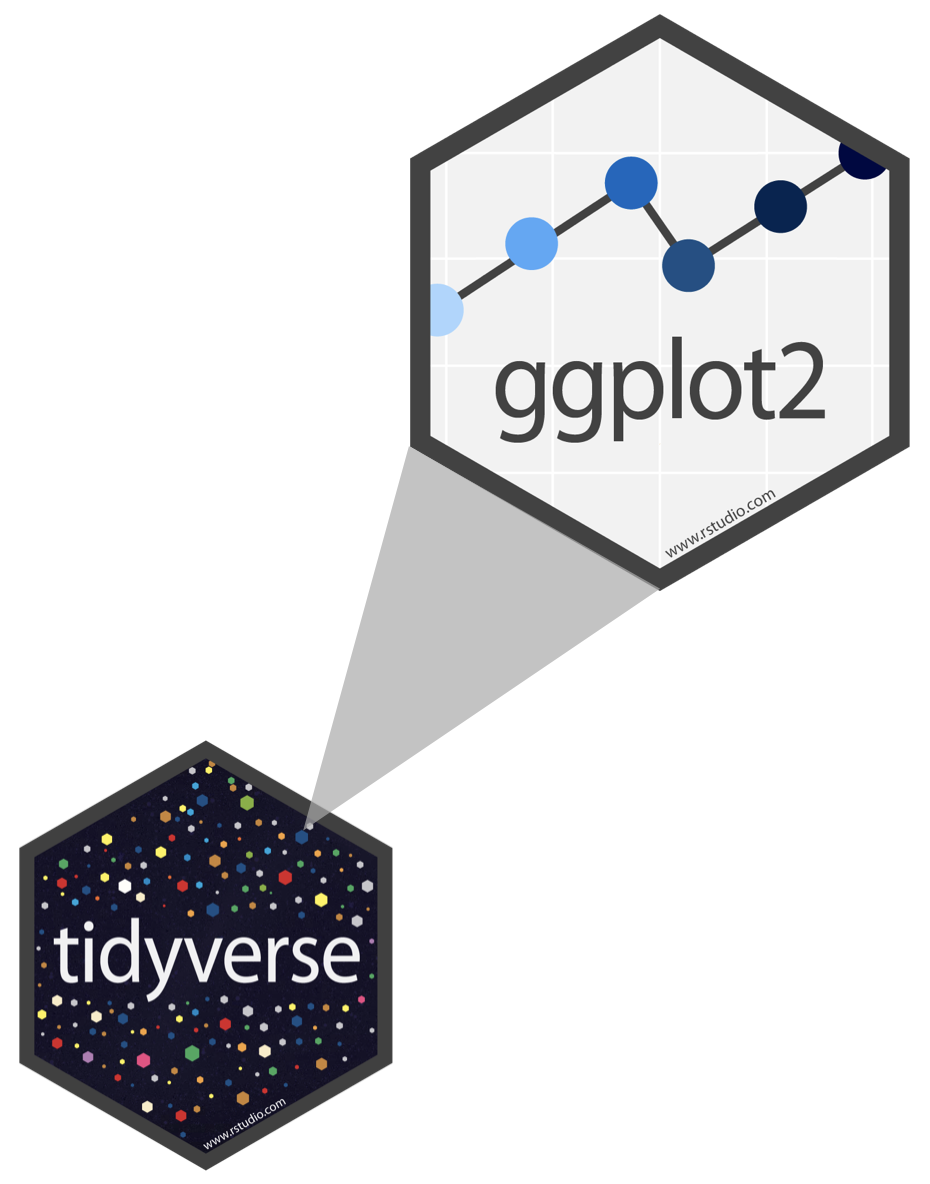
\includegraphics[width=2in,height=\textheight]{images/ggplot2-part-of-tidyverse.png}

}

\caption{\{ggplot2\} is one of the core packages of the \{tidyverse\}
metapackage. It is the most popular R package for data visualization.}

\end{figure}

Let's dive in!

\hypertarget{learning-objectives}{%
\section{Learning objectives}\label{learning-objectives}}

By the end of this lesson you should be able to:

\begin{enumerate}
\def\labelenumi{\arabic{enumi}.}
\item
  Recall and explain how the \textbf{\{ggplot2\}} package for data
  visualization is based on a theoretical framework called the
  \textbf{grammar of graphics}.
\item
  Name and describe the 3 essential components required for building a
  graph: \textbf{data}, \textbf{aesthetics}, and \textbf{geometries}.
\item
  Write code to \textbf{build a complete \texttt{ggplot}}
  \textbf{graphic} by correctly supplying the 3 essential layers to the
  \textbf{\texttt{ggplot()}} \textbf{function}.
\item
  Create different types of plots such as \textbf{scatter plots},
  \textbf{line graphs}, and \textbf{bar graphs}.
\item
  Add or modify visual elements of a plot such as \textbf{color} and
  \textbf{size}.
\item
  Distinguish between between \textbf{aesthetic mappings} and
  \textbf{fixed aesthetics}, and how to apply them.
\end{enumerate}

\begin{figure}

{\centering 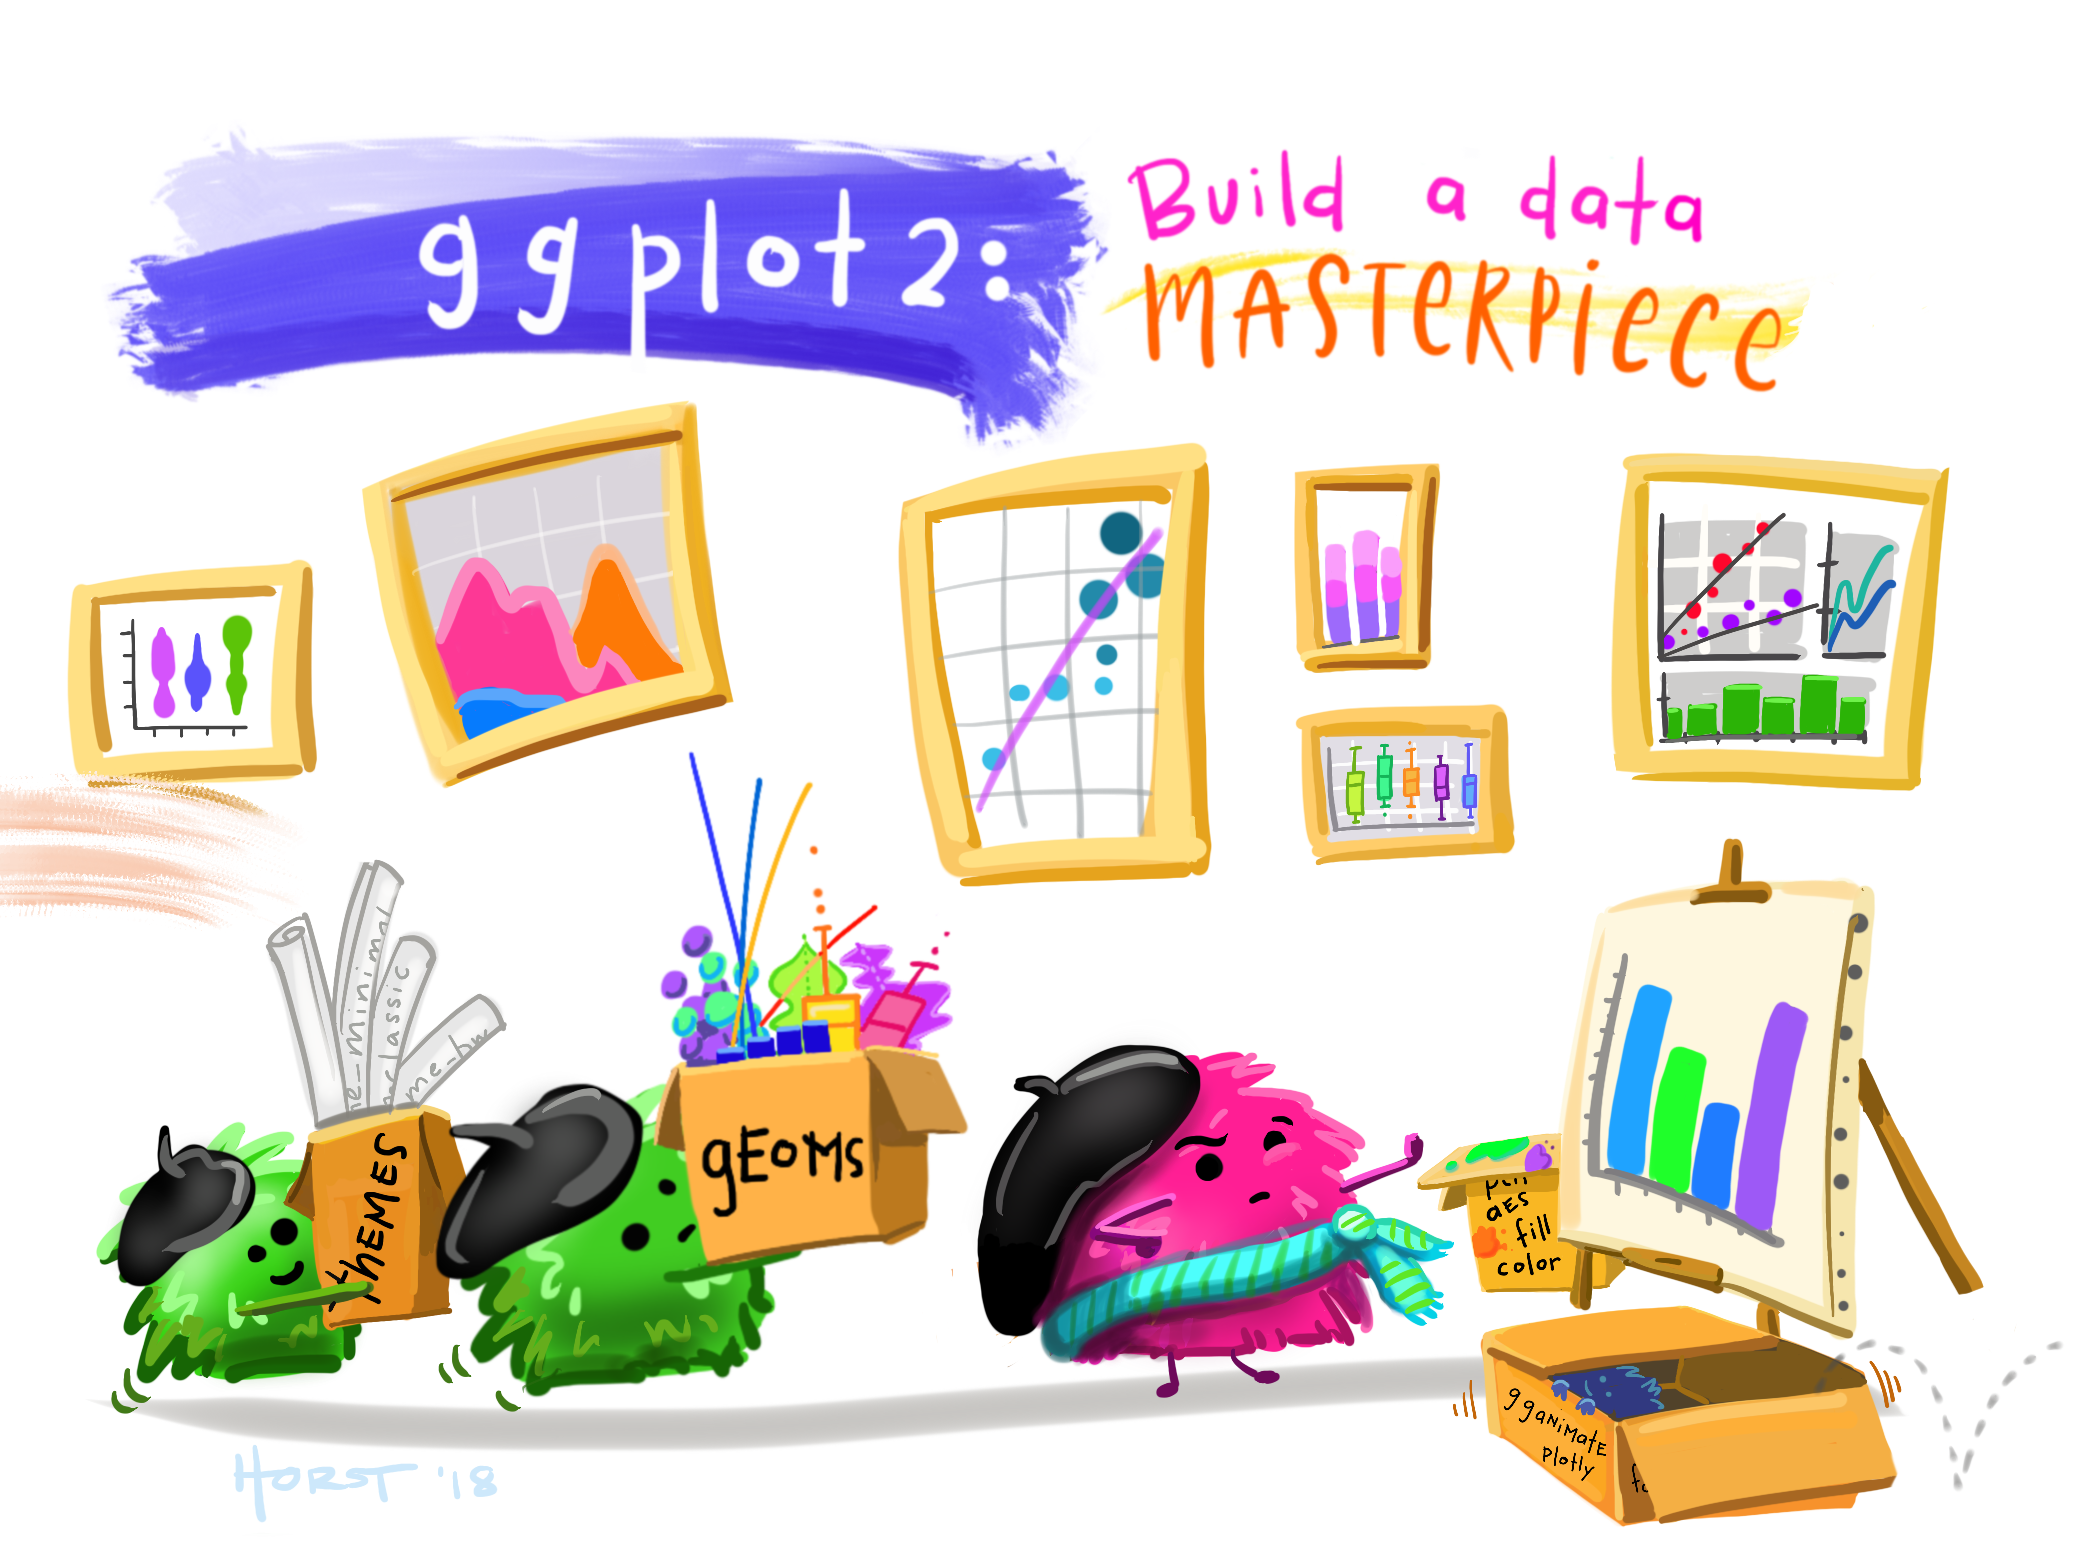
\includegraphics[width=6.25in,height=\textheight]{images/ggplot2_masterpiece.png}

}

\caption{Illustration by Allison Horst}

\end{figure}

\hypertarget{packages}{%
\section{Packages}\label{packages}}

The \{tidyverse\} meta package includes \{ggplot2\}, so we don't need to
add it separately. The \{here\} package will help us correctly reference
file paths.

\begin{Shaded}
\begin{Highlighting}[]
\DocumentationTok{\#\# Load packages }
\NormalTok{pacman}\SpecialCharTok{::}\FunctionTok{p\_load}\NormalTok{(tidyverse,}
\NormalTok{               here)}
\end{Highlighting}
\end{Shaded}

\hypertarget{measles-outbreaks-in-niger}{%
\section{Measles outbreaks in Niger}\label{measles-outbreaks-in-niger}}

In this lesson, we will explore patterns of measles outbreaks in Niger.

Measles is a \textbf{highly infectious virus} spread by airborne
respiratory droplets.

{[}Slide presentation about geography{]}

Since it is transmitted through direct contact, \textbf{population
density} is an important driver of measles dynamics.

\hypertarget{the-nigerm-dataset}{%
\subsection{\texorpdfstring{The \texttt{nigerm}
dataset}{The nigerm dataset}}\label{the-nigerm-dataset}}

We will be creating plots with a dataset of weekly reported measles
cases at the region level in Niger.

These data were collected by the Ministry of Health of Niger, from 1 Jan
1995 to 31 Dec 2005.

To get started, let's first load the (preprocessed) data set:

\begin{Shaded}
\begin{Highlighting}[]
\DocumentationTok{\#\# Import data frame to RStudio Environment}
\FunctionTok{load}\NormalTok{(}\FunctionTok{here}\NormalTok{(}\StringTok{"data/clean/nigerm\_cases\_rgn.RData"}\NormalTok{))}
\end{Highlighting}
\end{Shaded}

Take a moment to browse through the data:

\begin{Shaded}
\begin{Highlighting}[]
\DocumentationTok{\#\# Print Niger measles (nigerm) data frame}
\NormalTok{nigerm}
\end{Highlighting}
\end{Shaded}

\begin{figure}[H]

{\centering \includegraphics{data_on_display_ls01_gg_intro_files/figure-pdf/unnamed-chunk-5-1.pdf}

}

\end{figure}

The \textbf{\texttt{nigerm}} data frame has 4 variables (or columns):

\begin{enumerate}
\def\labelenumi{\arabic{enumi}.}
\item
  \textbf{\texttt{year}}: Calendar year (ranges from 1995 to 2005)
\item
  \textbf{\texttt{week}}: Week of the year (ranges from 1 to 52)
\item
  \textbf{\texttt{region}}: Region in which the cases were recorded (see
  figure below)
\item
  \textbf{\texttt{cases}}: Number of measles cases reported
\end{enumerate}

\begin{figure}

{\centering 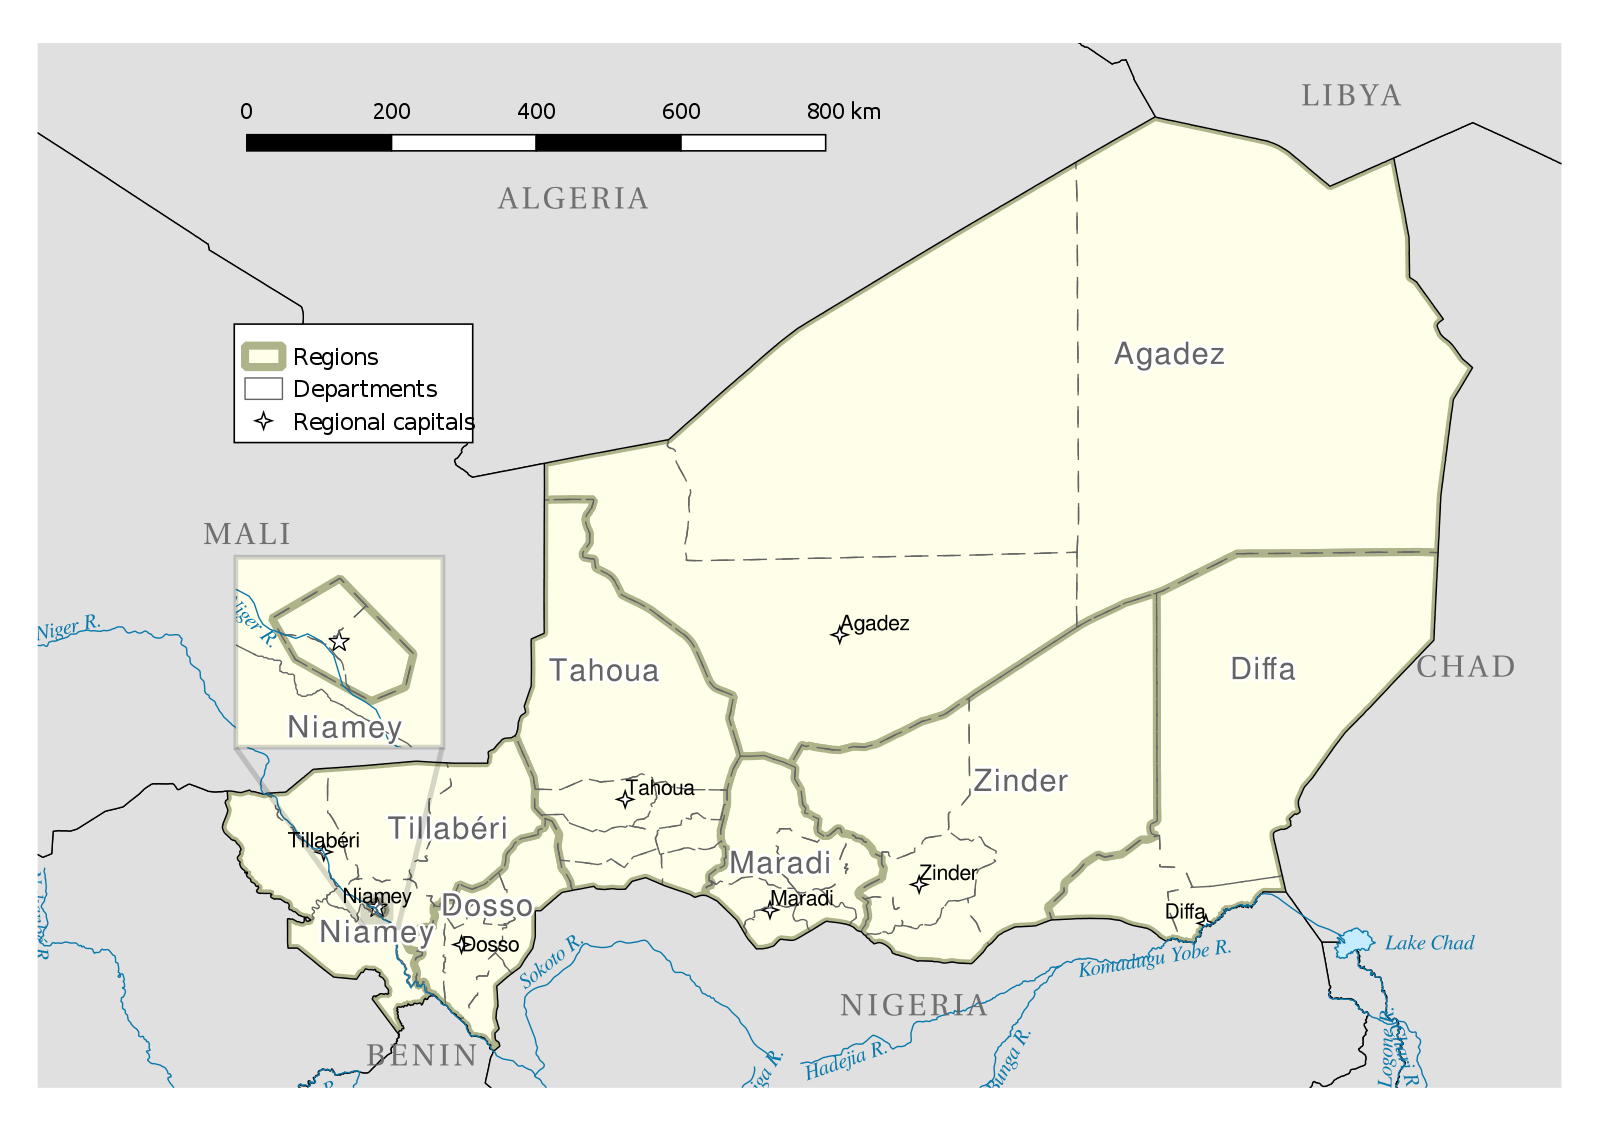
\includegraphics{images/niger_administrative_divisions.png}

}

\caption{Administrative divisions of Niger: Districts and Regions}

\end{figure}

Several papers have investigated these trends, linking measles to human
activity, migration, and seasonality.

\begin{figure}

{\centering 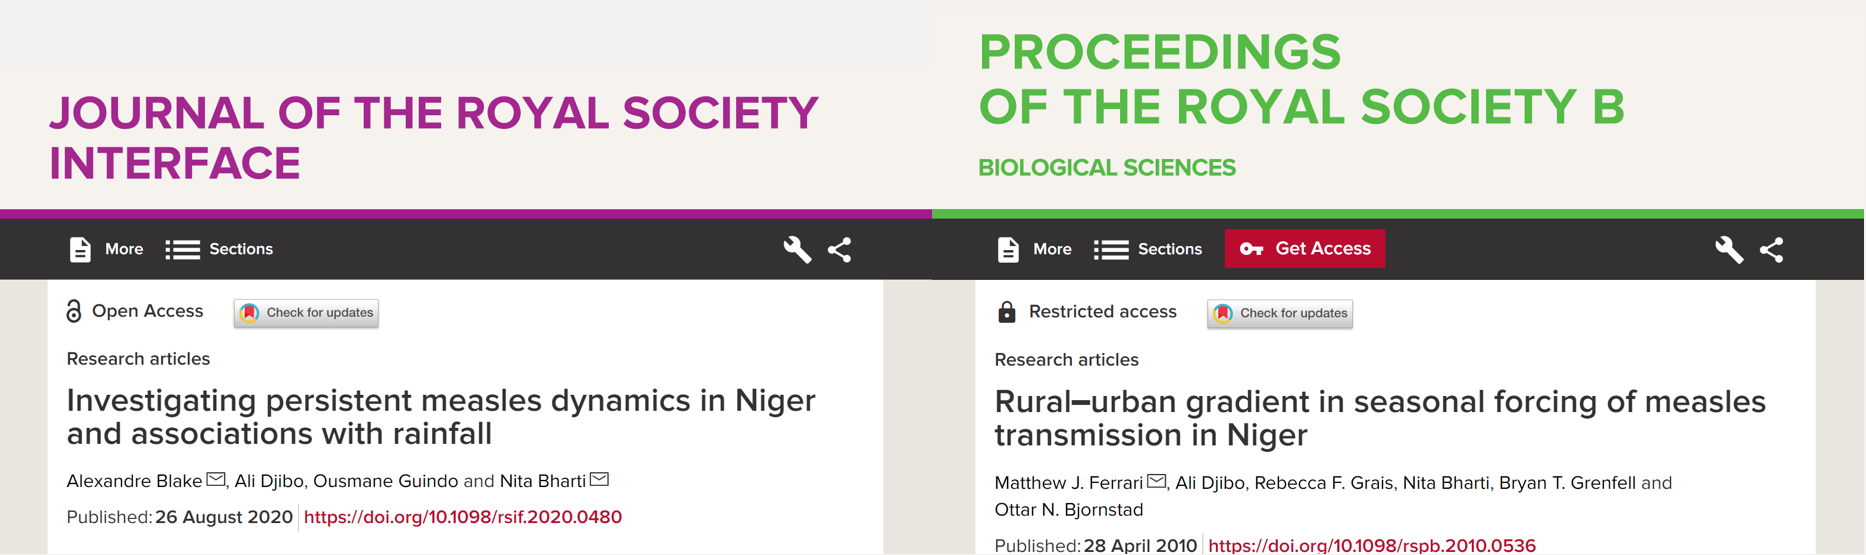
\includegraphics{images/paste-B863326A.png}

}

\caption{Research articles that have used this dataset, and analyzed it
in R!}

\end{figure}

These studies are much more complex than what we will do there, but
let's see if we can find any patterns even with basic
\textbf{exploratory data visualization}.

We can get some information about patterns in this data by inspecting
summary statistics given by the \textbf{\texttt{summary()}} function:

\begin{Shaded}
\begin{Highlighting}[]
\FunctionTok{summary}\NormalTok{(nigerm)}
\end{Highlighting}
\end{Shaded}

\begin{verbatim}
      year           week           region         cases       
 Min.   :1995   Min.   : 1.00   Agadez : 572   Min.   :   0.0  
 1st Qu.:1997   1st Qu.:13.75   Diffa  : 572   1st Qu.:   1.0  
 Median :2000   Median :26.50   Dosso  : 572   Median :  16.0  
 Mean   :2000   Mean   :26.50   Maradi : 572   Mean   : 100.3  
 3rd Qu.:2003   3rd Qu.:39.25   Niamey : 572   3rd Qu.:  86.0  
 Max.   :2005   Max.   :52.00   Tahoua : 572   Max.   :1887.0  
                                (Other):1144                   
\end{verbatim}

This gives us values for the maximum, minimum, and quartiles of each
numeric variable, and the number of observations (rows) for each region.
This is summary useful, but it omits a large amount information
contained in the dataset.

Keep in mind that summary statistics can be highly misleading, and a
simple plot can reveal a lot more.

The easiest and clearest way to analyze patterns from this dataset is to
visualize it!

The best way to do this in R is with \{ggplot2\}. So let's see how that
works.

\hypertarget{the-layered-grammar-of-graphics}{%
\subsection{The layered Grammar of
Graphics}\label{the-layered-grammar-of-graphics}}

The \texttt{gg} in \texttt{ggplot} is short for ``\texttt{g}rammar of
\texttt{g}raphics'', which is the data visualization philosophy that
\{ggplot2\} is based on.

The \textbf{grammar of graphics} is a theoretical framework which
deconstructs the process of producing a graph.

Think of how we construct and form sentences in written and spoken
languages by combining different elements, like nouns, verbs, articles,
subjects, objects, etc. We can't just combine these elements in any
arbitrary order; we must do so following a set of rules known as a
linguistic grammar.

Similarly, the grammar of graphics (GG) defines a set of rules for
constructing \emph{graphics} by combining different types of elements,
known as \emph{layers}.

\begin{figure}

{\centering 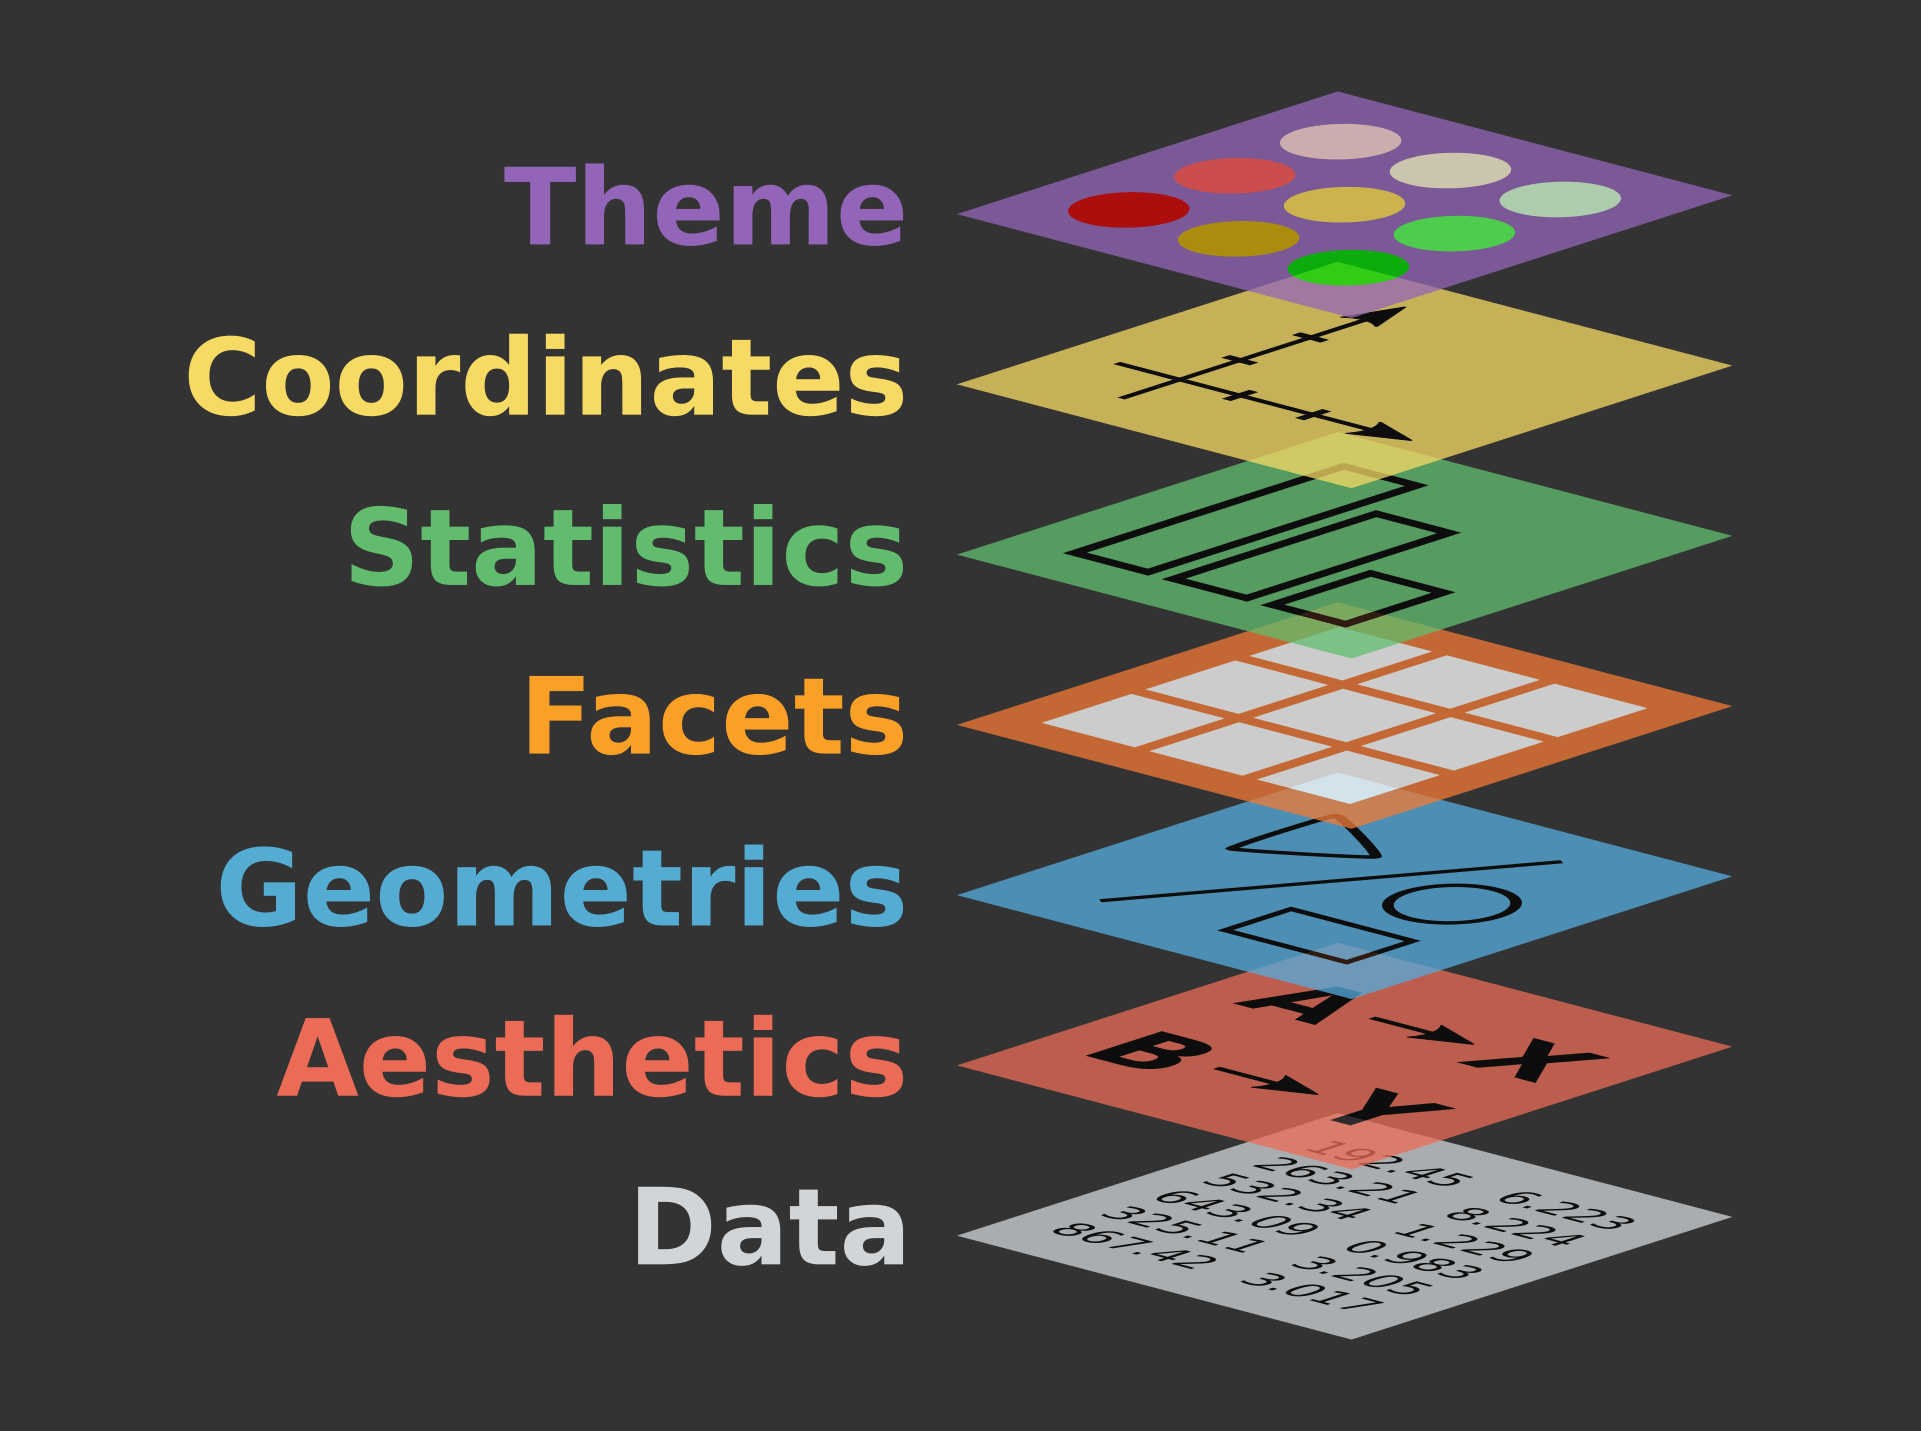
\includegraphics[width=4.08333in,height=\textheight]{images/gglayers.png}

}

\caption{The grammar of graphics framework dissects a graph into
individual components, which belong to these seven distinct layers. We
take these different layers and combine them together to build a plot.}

\end{figure}

The three layers at the bottom of this figure - \textbf{data},
\textbf{aesthetics}, and \textbf{geometries} - are required for building
any plot.

Let's define what they mean:

\begin{enumerate}
\def\labelenumi{\arabic{enumi}.}
\item
  \textbf{\texttt{data}}: the dataset containing the variables of
  interest.

  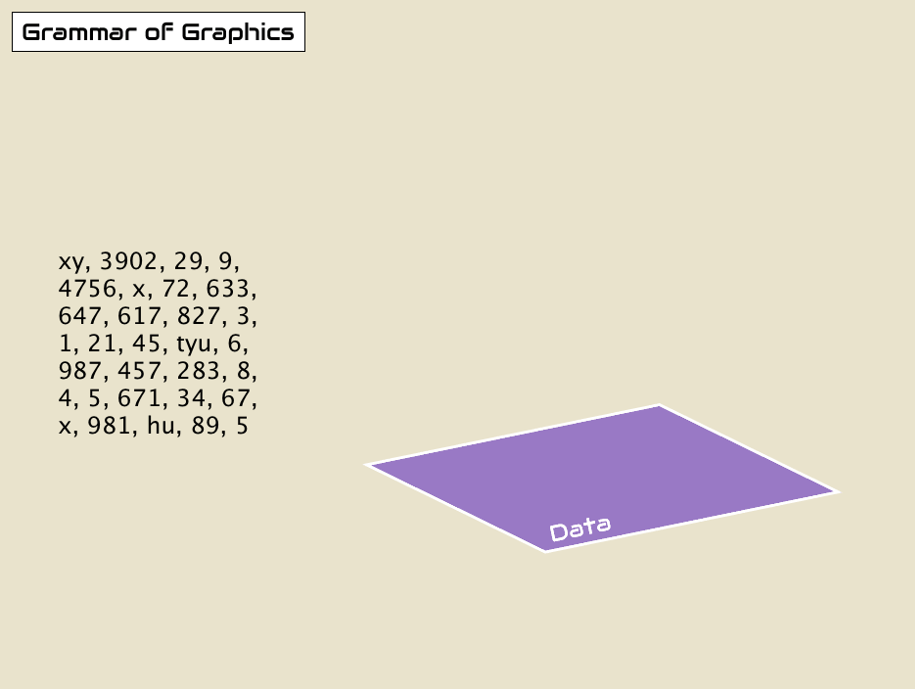
\includegraphics[width=4.6875in,height=\textheight]{images/gglayers_data.png}
\item
  \textbf{\texttt{aes}}thetics: things we can see that visually
  communicate information in our data.

  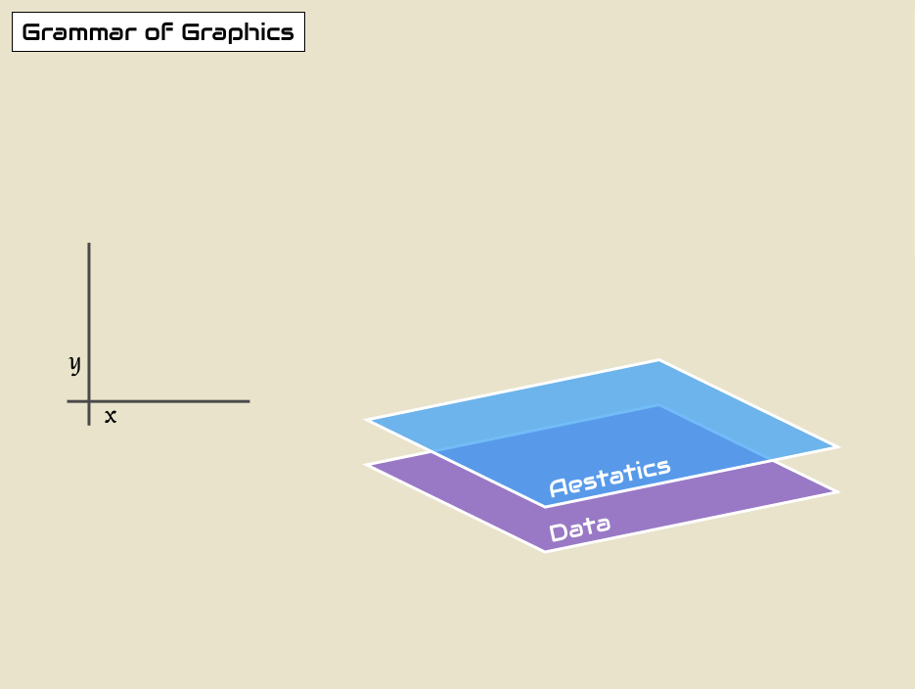
\includegraphics[width=4.6875in,height=\textheight]{images/gglayers_aes.png}
\item
  \textbf{\texttt{geom}}etry: the geometric shape used to represent data
  in a plot: points, lines, bars, etc.

  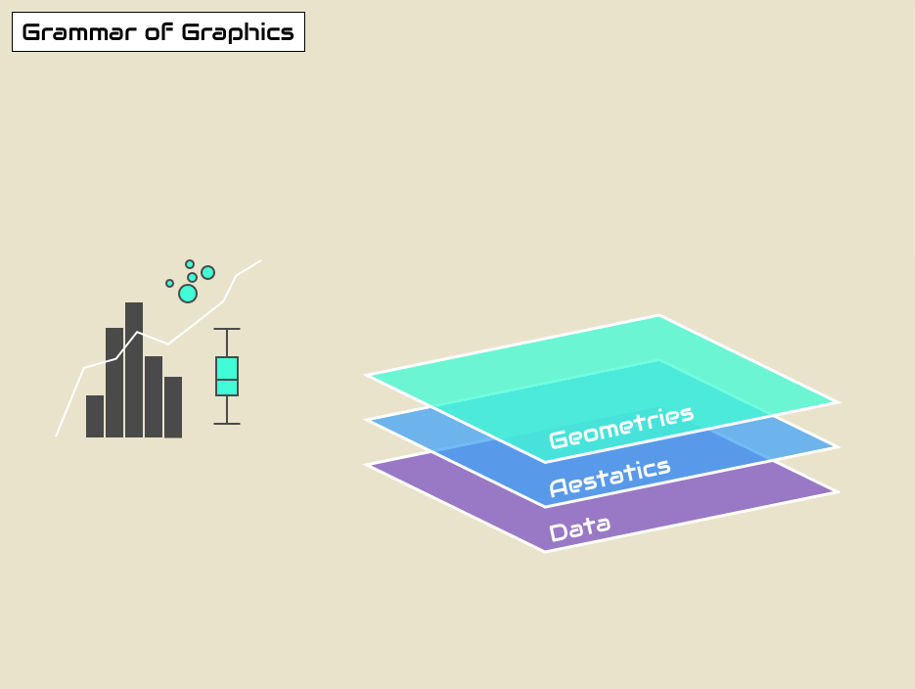
\includegraphics[width=4.6875in,height=\textheight]{images/gglayers_geom.png}
\end{enumerate}

You might be wondering why we wrote \texttt{data}, \texttt{geom}, and
\texttt{aes} in a computer code type font. You'll see very shortly that
we use these terms in R code to represent GG layers.

\begin{tcolorbox}[enhanced jigsaw, colframe=quarto-callout-note-color-frame, colbacktitle=quarto-callout-note-color!10!white, titlerule=0mm, opacitybacktitle=0.6, breakable, toprule=.15mm, arc=.35mm, rightrule=.15mm, colback=white, bottomrule=.15mm, opacityback=0, toptitle=1mm, left=2mm, bottomtitle=1mm, title=\textcolor{quarto-callout-note-color}{\faInfo}\hspace{0.5em}{Challenge}, leftrule=.75mm, coltitle=black]

The terms and syntax used for \texttt{ggplot} functions, arguments, and
layers can be hard to keep up with at first, but as you gain experience
using these terms to make plots in R, you will become fluent in no time.

\end{tcolorbox}

\hypertarget{working-through-the-essential-layers}{%
\section{Working through the essential
layers}\label{working-through-the-essential-layers}}

In this section, we will work towards a first plot with \{ggplot2\}. It
will be a scatter plot using data from \texttt{nigerm}.

For easier plotting in this lesson, we will use a smaller subsets of the
\texttt{nigerm} data frame at a time.

First let's create one called \texttt{nigerm96}, which only contains
measles case data for the year 1996. Running the code below will create
\texttt{nigerm96} and add it to your RStudio Environment:

\begin{Shaded}
\begin{Highlighting}[]
\DocumentationTok{\#\# Create nigerm96 data frame}
\NormalTok{nigerm96 }\OtherTok{\textless{}{-}}\NormalTok{ nigerm }\SpecialCharTok{\%\textgreater{}\%}   
  \FunctionTok{filter}\NormalTok{(year }\SpecialCharTok{==} \DecValTok{1996}\NormalTok{)  }\SpecialCharTok{\%\textgreater{}\%} \CommentTok{\# filter to only include rows from 1996}
  \FunctionTok{select}\NormalTok{(}\SpecialCharTok{{-}}\NormalTok{year) }\CommentTok{\# remove the year column}
\end{Highlighting}
\end{Shaded}

\begin{tcolorbox}[enhanced jigsaw, colframe=quarto-callout-note-color-frame, colbacktitle=quarto-callout-note-color!10!white, titlerule=0mm, opacitybacktitle=0.6, breakable, toprule=.15mm, arc=.35mm, rightrule=.15mm, colback=white, bottomrule=.15mm, opacityback=0, toptitle=1mm, left=2mm, bottomtitle=1mm, title=\textcolor{quarto-callout-note-color}{\faInfo}\hspace{0.5em}{Reminder}, leftrule=.75mm, coltitle=black]

The \texttt{select()} and \texttt{filter()} functions are part of the
\{dplyr\} package for data manipulation, which is a core package of the
\{tidyverse\}. These topics are covered in the Data Wrangling course.
See The GRAPH Courses \href{https://thegraphcourses.org/}{website} for
more.

\end{tcolorbox}

Let's look at our new dataframe, \texttt{nigerm96}:

\begin{Shaded}
\begin{Highlighting}[]
\DocumentationTok{\#\# Print nigerm96}
\NormalTok{nigerm96}
\end{Highlighting}
\end{Shaded}

\begin{figure}[H]

{\centering \includegraphics{data_on_display_ls01_gg_intro_files/figure-pdf/unnamed-chunk-8-1.pdf}

}

\end{figure}

\hypertarget{building-a-ggplot-in-steps}{%
\subsection{\texorpdfstring{Building a \texttt{ggplot()} in
steps}{Building a ggplot() in steps}}\label{building-a-ggplot-in-steps}}

Time to start building a \texttt{ggplot} in increments! We'll do this by
starting with a blank canvas and then adding one layer at a time.

\textbf{Step 0: Call the \texttt{ggplot()} function}

\begin{Shaded}
\begin{Highlighting}[]
\DocumentationTok{\#\# Call the \textasciigrave{}ggplot()\textasciigrave{} function}
\FunctionTok{ggplot}\NormalTok{()}
\end{Highlighting}
\end{Shaded}

\begin{figure}[H]

{\centering 
\includegraphics{data_on_display_ls01_gg_intro_files/figure-pdf/unnamed-chunk-9-1.pdf}

}

\end{figure}

As you can see, this gives us nothing but a blank canvas. But not to
worry, we're about to add some more elements.

\textbf{Step 1: Provide data}

The first input we need to supply the \texttt{ggplot()} function is the
data layer (i.e., a data frame), by filling in the \texttt{data}
argument (\texttt{data\ =\ DF\_NAME}):

\begin{Shaded}
\begin{Highlighting}[]
\DocumentationTok{\#\# Data layer}
\FunctionTok{ggplot}\NormalTok{(}\AttributeTok{data =}\NormalTok{ nigerm96)  }\CommentTok{\# what data to use}
\end{Highlighting}
\end{Shaded}

\begin{figure}[H]

{\centering 
\includegraphics{data_on_display_ls01_gg_intro_files/figure-pdf/unnamed-chunk-10-1.pdf}

}

\end{figure}

This gives us blank plot again, since we've only supplied one out of the
three inputs required for a complete graphic. Next we need to assign
variables to aesthetic mappings.

\textbf{Step 2: Define the variables}

What should we plot on our axes? Let's say we want to make an epidemic
time series plot. To do that, we plot time (in weeks) on the x-axis, and
disease incidence (number of reported cases) on the y-axis. In
\texttt{ggplot}-speak, we are \texttt{mapping} the variable
\texttt{cases} to the \texttt{x} aesthetic, and \texttt{week} to the
\texttt{y} aesthetic.

Let's tell \texttt{ggplot()} which variables to to plot on the
aesthetics layer with a \texttt{mapping} argument, using this syntax:
\texttt{mapping\ =\ aes(x\ =\ VAR1,\ y\ =\ VAR2)}.

\begin{Shaded}
\begin{Highlighting}[]
\DocumentationTok{\#\# Aesthetics layer: x and y position}
\FunctionTok{ggplot}\NormalTok{(}\AttributeTok{data =}\NormalTok{ nigerm96, }\CommentTok{\# what data to use}
       \AttributeTok{mapping =} \FunctionTok{aes}\NormalTok{(   }\CommentTok{\# supply a mapping in the form of an \textquotesingle{}aesthetic\textquotesingle{}}
         \AttributeTok{x =}\NormalTok{ week,      }\CommentTok{\# which variable to map onto the x{-}axis}
         \AttributeTok{y =}\NormalTok{ cases))    }\CommentTok{\# which variable to map onto the y{-}axis}
\end{Highlighting}
\end{Shaded}

\begin{figure}[H]

{\centering 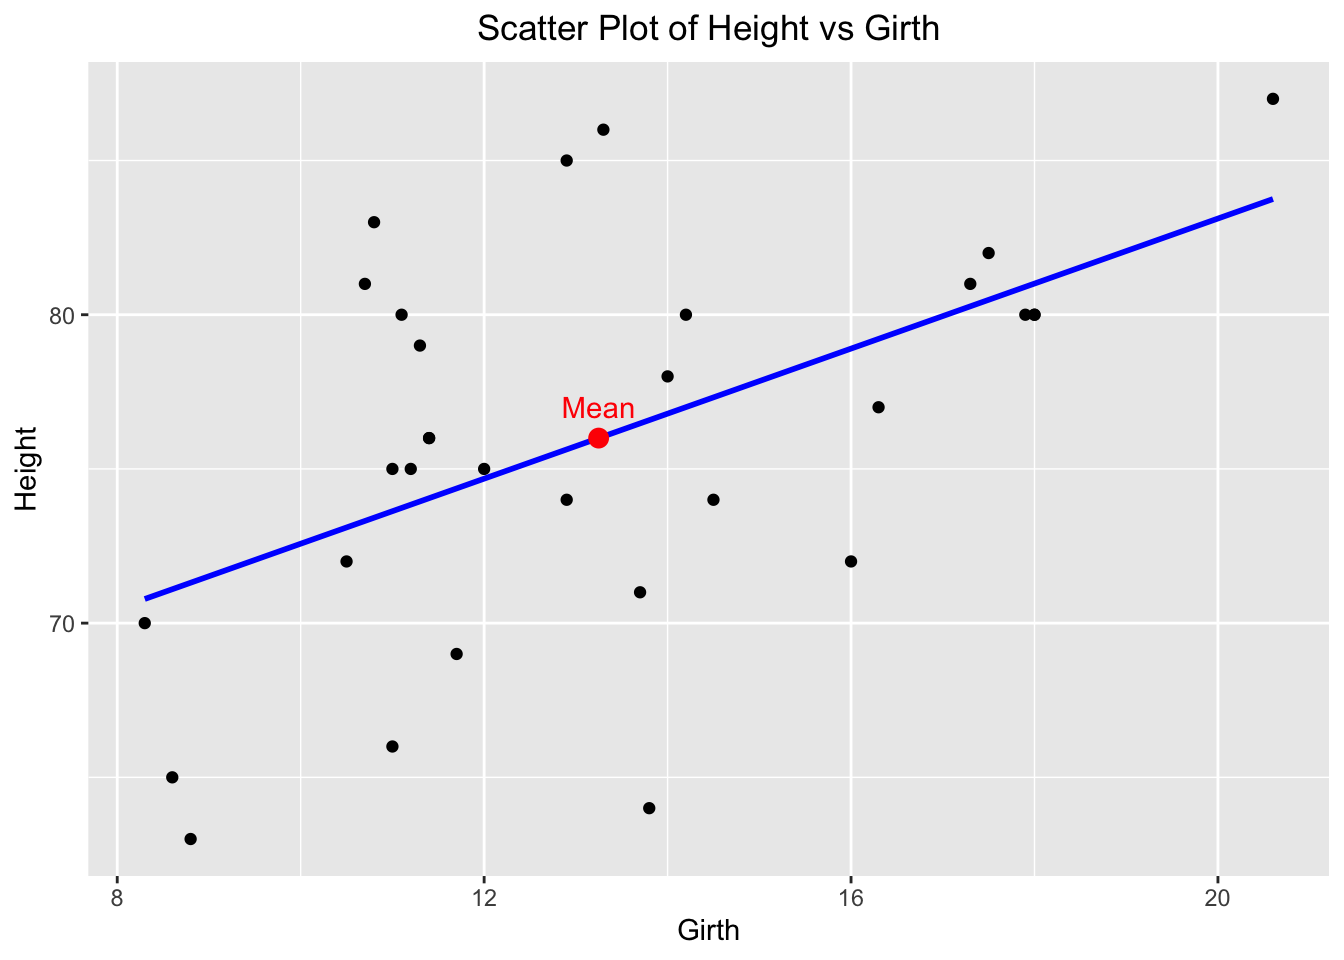
\includegraphics{data_on_display_ls01_gg_intro_files/figure-pdf/unnamed-chunk-11-1.pdf}

}

\end{figure}

There's still no data plotted, but the axis scales, titles, and labels
are present. The x-axis marks weeks of the year from 1 to 52, and the
y-axis shows that the number of weekly reported cases per region ranges
from 0 to around 2000.

The plot is still lacking the required geometry layer.

\begin{tcolorbox}[enhanced jigsaw, colframe=quarto-callout-note-color-frame, colbacktitle=quarto-callout-note-color!10!white, titlerule=0mm, opacitybacktitle=0.6, breakable, toprule=.15mm, arc=.35mm, rightrule=.15mm, colback=white, bottomrule=.15mm, opacityback=0, toptitle=1mm, left=2mm, bottomtitle=1mm, title=\textcolor{quarto-callout-note-color}{\faInfo}\hspace{0.5em}{Key Point}, leftrule=.75mm, coltitle=black]

\texttt{aes()} stands for aesthetics - things we can see. Variables are
always inside the \texttt{aes()} function, which in return is inside a
\texttt{ggplot()}. Take a moment to observe the double closing brackets
\textbf{\texttt{))}} - the first one belongs to \texttt{aes()}, the
second one to \texttt{ggplot()}.

\end{tcolorbox}

\textbf{Step 3: Specify which type of plot to create}

Finally, we add a geometry layer using a \texttt{geom\_*} function. This
determines which geometric objects - or visual markers - should be used
to map the data.

Since we are looking at the relationship of two numerical variables, it
makes sense to use a \textbf{scatter plot}. The geometric objects used
to represent data on scatter plots are \textbf{points}, and the
\texttt{geom\_*} function for scatter plots is conveniently named
\textbf{\texttt{geom\_point()}}. We'll add this function as new layer
using a \textbf{\texttt{+}} sign:

\begin{Shaded}
\begin{Highlighting}[]
\DocumentationTok{\#\# Geometries layer: points}
\FunctionTok{ggplot}\NormalTok{(}\AttributeTok{data =}\NormalTok{ nigerm96, }\CommentTok{\# what data to use}
       \AttributeTok{mapping =} \FunctionTok{aes}\NormalTok{(   }\CommentTok{\# define mapping}
         \AttributeTok{x =}\NormalTok{ week,      }\CommentTok{\# which variable to map onto the x{-}axis}
         \AttributeTok{y =}\NormalTok{ cases)) }\SpecialCharTok{+}  \CommentTok{\# which variable to map onto the y{-}axis}
  \FunctionTok{geom\_point}\NormalTok{()          }\CommentTok{\# add a geom of type \textasciigrave{}point\textasciigrave{} (for scatter plot)}
\end{Highlighting}
\end{Shaded}

\begin{figure}[H]

{\centering 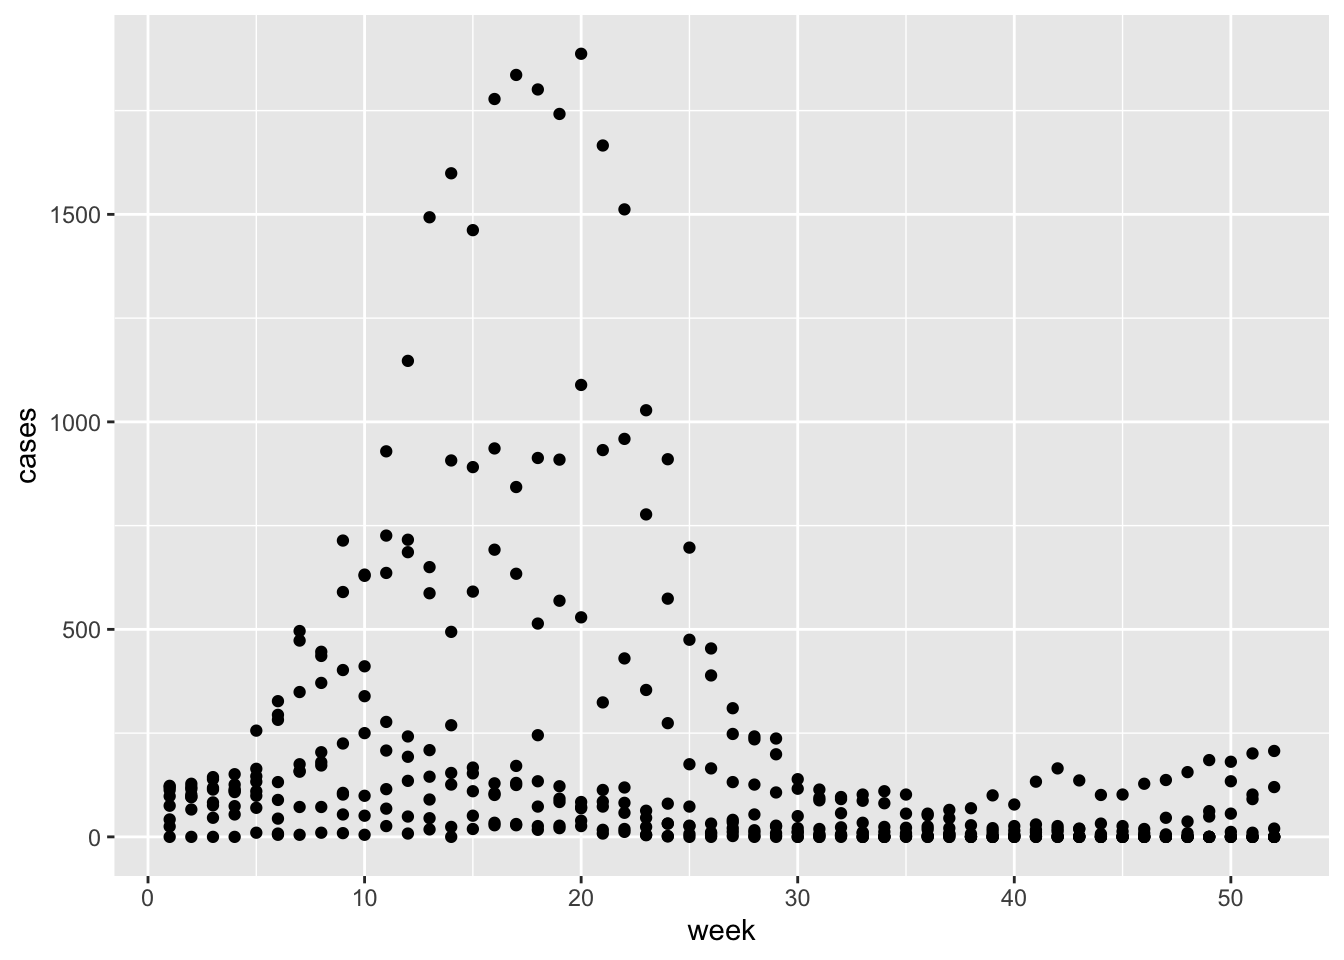
\includegraphics{data_on_display_ls01_gg_intro_files/figure-pdf/unnamed-chunk-12-1.pdf}

}

\end{figure}

Points have been added, and this is now a complete scatter plot! There
are 8 points per week, representing each of the 8 regions (but at this
point we cannot tell which point is from which region).

\begin{tcolorbox}[enhanced jigsaw, colframe=quarto-callout-note-color-frame, colbacktitle=quarto-callout-note-color!10!white, titlerule=0mm, opacitybacktitle=0.6, breakable, toprule=.15mm, arc=.35mm, rightrule=.15mm, colback=white, bottomrule=.15mm, opacityback=0, toptitle=1mm, left=2mm, bottomtitle=1mm, title=\textcolor{quarto-callout-note-color}{\faInfo}\hspace{0.5em}{Reminder}, leftrule=.75mm, coltitle=black]

The \texttt{aes}thetic function is nested inside the \texttt{ggplot()}
function, so be sure to close the brackets for both functions before
adding the \texttt{+} sign for the \texttt{geom\_*} function, or your
code will not run correctly.

\end{tcolorbox}

It's your turn to practice plotting with \texttt{ggplot()}! For practice
exercises in this lesson, you will be using a different subset of
\texttt{nigerm} called \textbf{\texttt{nigerm04}}, which contains only
data from the year 2004:

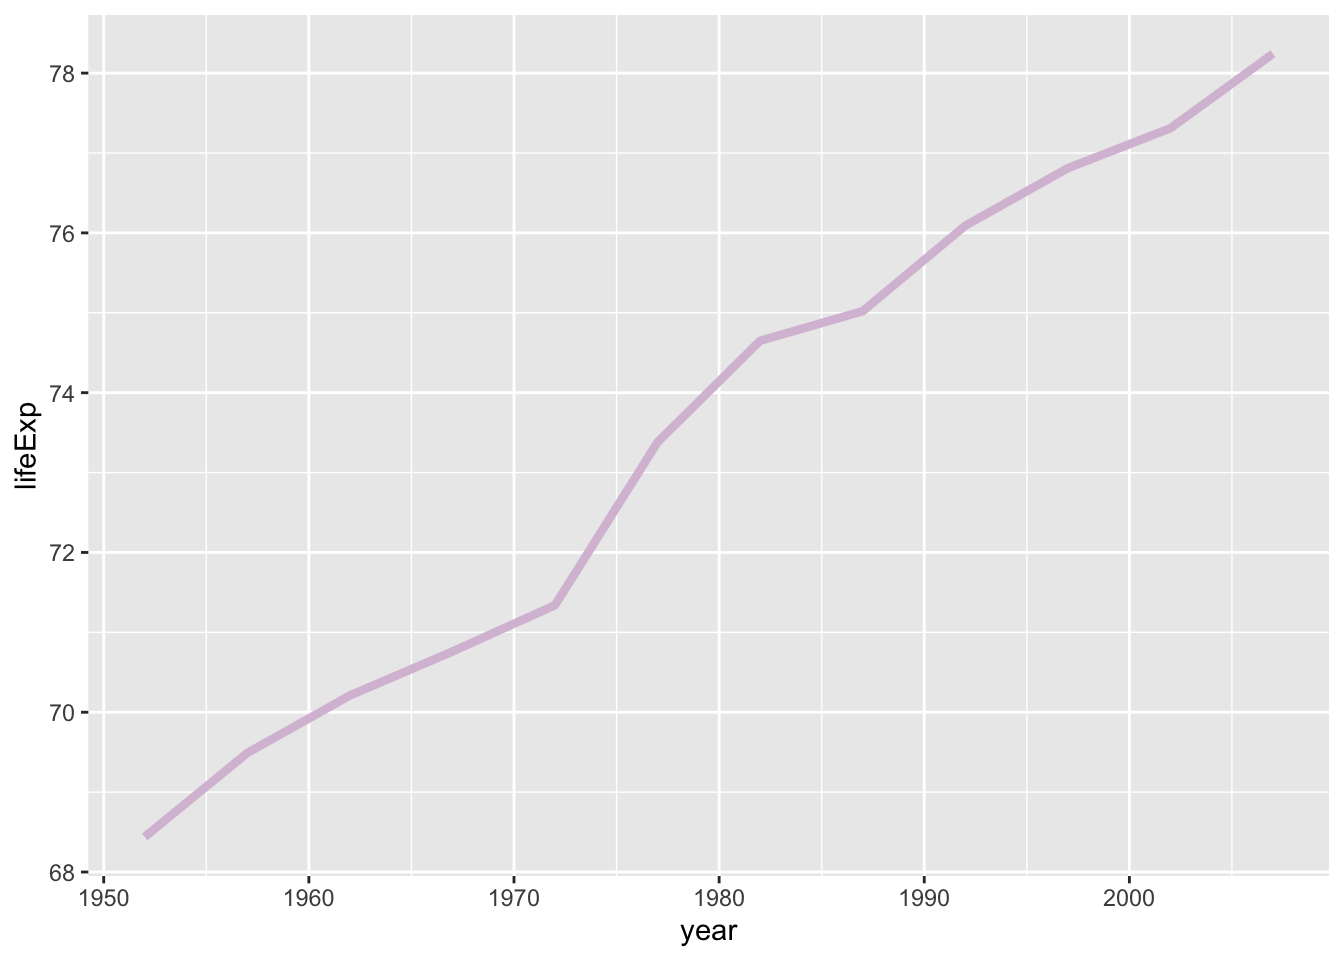
\includegraphics{data_on_display_ls01_gg_intro_files/figure-pdf/unnamed-chunk-13-1.pdf}

Plotting with a different set of data will also allow you to explore if
the patterns we see for 1996 is also true for 2004.

\begin{tcolorbox}[enhanced jigsaw, colframe=quarto-callout-tip-color-frame, colbacktitle=quarto-callout-tip-color!10!white, titlerule=0mm, opacitybacktitle=0.6, breakable, toprule=.15mm, arc=.35mm, rightrule=.15mm, colback=white, bottomrule=.15mm, opacityback=0, toptitle=1mm, left=2mm, bottomtitle=1mm, title=\textcolor{quarto-callout-tip-color}{\faLightbulb}\hspace{0.5em}{Practice}, leftrule=.75mm, coltitle=black]

Using the \texttt{nigerm04} data frame, write \texttt{ggplot} code that
will create a scatter plot displaying the relationship between
\texttt{cases} on the y-axis and \texttt{week} on the x-axis.

\end{tcolorbox}

\hypertarget{modifying-the-layers}{%
\section{Modifying the layers}\label{modifying-the-layers}}

Generally speaking, the grammar of graphics allows for a high degree of
customization of plots and also a consistent framework for easily
updating and modifying them.

We can tinker with our existing code to switch up the data, aesthetics,
and geometry inputs supplied to \texttt{ggplot()}, and create variations
of the original plot. In fact, you've already done this by changing the
dataset from \texttt{nigerm96} to \texttt{nigerm04} in the practice
question.

Similarly, the \texttt{aes}thetics and \texttt{geom}etry inputs can also
be changed to create different visualizations. In the next few sections
we will take the scatter plot we built in the previous section, and make
incremental changes to modify different elements of the original code.

\hypertarget{changing-aesthetic-mappings}{%
\subsection{\texorpdfstring{Changing \texttt{aes}thetic
mappings}{Changing aesthetic mappings}}\label{changing-aesthetic-mappings}}

We created a scatter plot of \texttt{cases} vs \texttt{week} for
\texttt{nigerm96} with this code:

\begin{Shaded}
\begin{Highlighting}[]
\FunctionTok{ggplot}\NormalTok{(}\AttributeTok{data =}\NormalTok{ nigerm96, }
       \AttributeTok{mapping =} \FunctionTok{aes}\NormalTok{(}\AttributeTok{x =}\NormalTok{ week, }
                     \AttributeTok{y =}\NormalTok{ cases)) }\SpecialCharTok{+}
  \FunctionTok{geom\_point}\NormalTok{()}
\end{Highlighting}
\end{Shaded}

\begin{figure}[H]

{\centering 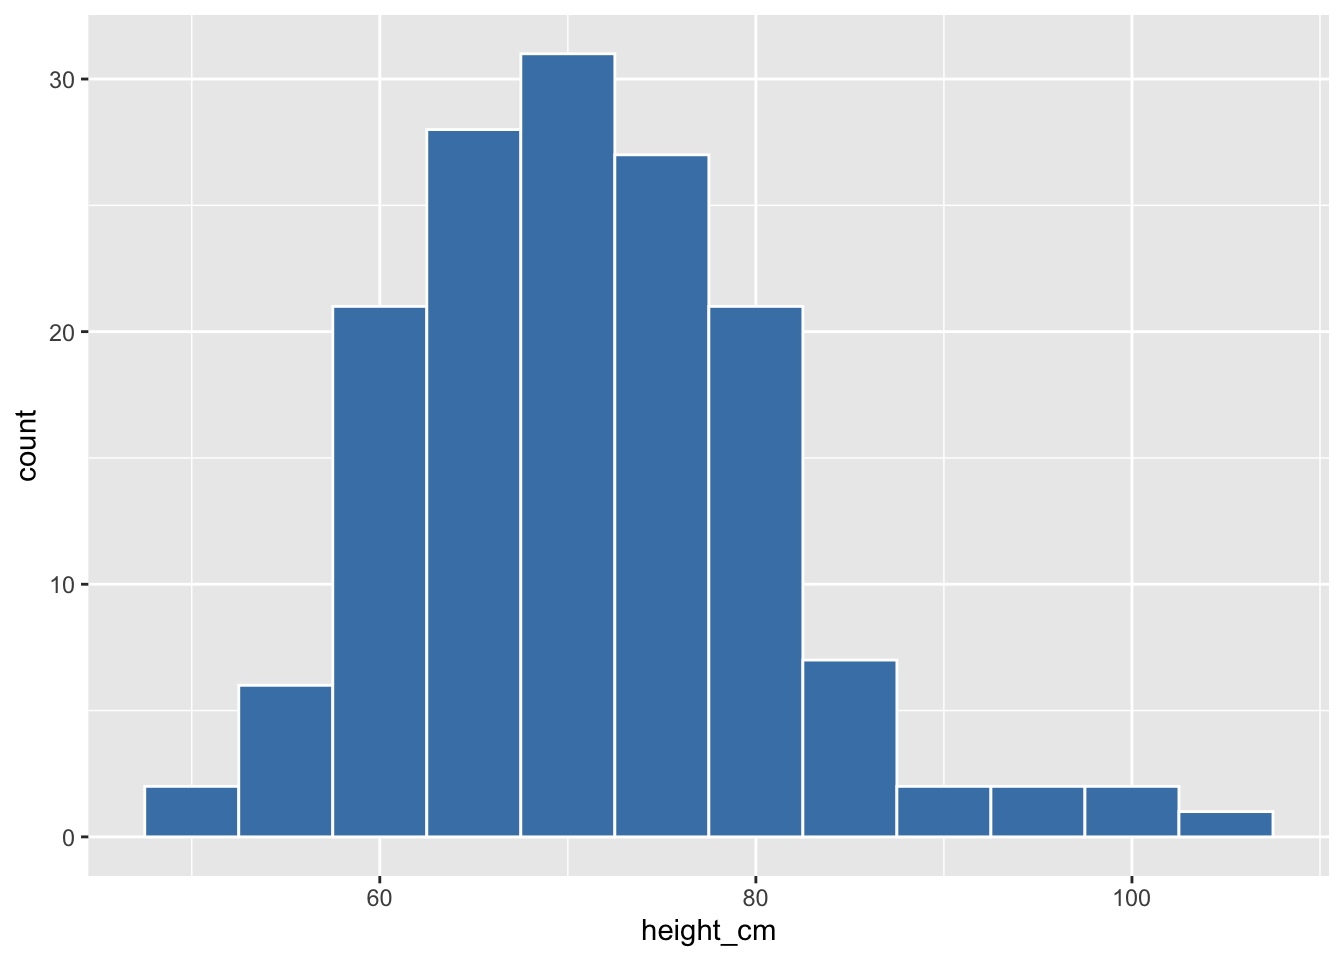
\includegraphics{data_on_display_ls01_gg_intro_files/figure-pdf/unnamed-chunk-19-1.pdf}

}

\end{figure}

If we copy the same code and change just one thing - by replacing the
\texttt{x} variable \texttt{week} (numerical) with \texttt{region}
(categorical) - we get what's called a \textbf{strip plot}:

\begin{Shaded}
\begin{Highlighting}[]
\FunctionTok{ggplot}\NormalTok{(}\AttributeTok{data =}\NormalTok{ nigerm96, }
       \AttributeTok{mapping =} \FunctionTok{aes}\NormalTok{(}\AttributeTok{x =}\NormalTok{ region, }\CommentTok{\# change which variable to map on the x{-}axis }
                     \AttributeTok{y =}\NormalTok{ cases)) }\SpecialCharTok{+}
  \FunctionTok{geom\_point}\NormalTok{()}
\end{Highlighting}
\end{Shaded}

\begin{figure}[H]

{\centering \includegraphics{data_on_display_ls01_gg_intro_files/figure-pdf/unnamed-chunk-20-1.pdf}

}

\end{figure}

While the y-axis values of the points are the same as before, their
x-axis mappings have changed significantly. They are now mapped to 8
separate positions along the x-axis, each corresponding to a discrete
category of the \texttt{region} variable.

\hypertarget{changing-geom_-functions}{%
\subsection{\texorpdfstring{Changing \texttt{geom\_*}
functions}{Changing geom\_* functions}}\label{changing-geom_-functions}}

Similarly, we can modify the geometry layer to create a different type
of plot, while still using the same aesthetic mappings.

\begin{figure}

{\centering 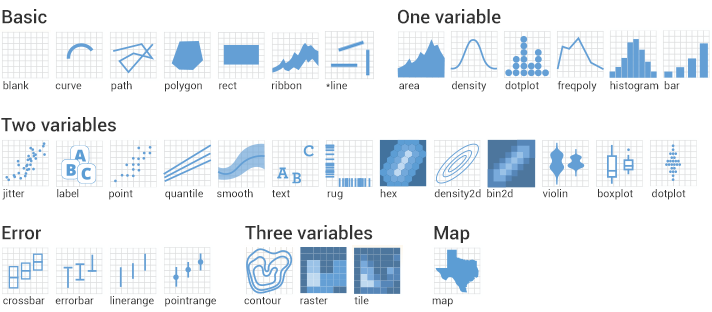
\includegraphics{images/geoms.png}

}

\caption{\{ggplot2\} has a variety of different \texttt{geom\_*}
functions and geometric objects which you can use to visualize your
data. Here are some examples of different types of geoms that can be
used with \texttt{ggplot()}.}

\end{figure}

Let's copy and paste the original scatter plot code once again, but this
time we will replace the \texttt{geom\_*} function instead of the
\texttt{x} aesthetic. If we change \texttt{geom\_point()} to
\textbf{\texttt{geom\_col()}}, we get a \textbf{bar plot} (sometimes
called a \texttt{col}umn chart):

\begin{Shaded}
\begin{Highlighting}[]
\FunctionTok{ggplot}\NormalTok{(}\AttributeTok{data =}\NormalTok{ nigerm96, }
       \AttributeTok{mapping =} \FunctionTok{aes}\NormalTok{(}\AttributeTok{x =}\NormalTok{ week,}
                     \AttributeTok{y =}\NormalTok{ cases)) }\SpecialCharTok{+}  
  \FunctionTok{geom\_col}\NormalTok{()  }\CommentTok{\# declare that we want a bar plot}
\end{Highlighting}
\end{Shaded}

\begin{figure}[H]

{\centering \includegraphics{data_on_display_ls01_gg_intro_files/figure-pdf/unnamed-chunk-21-1.pdf}

}

\end{figure}

Again, the rest of the code is still the same - we just changed the key
word of the \texttt{geom\_*} function. However, the plot is
significantly different that either the scatter plot or the strip plot.

Notice that the y-axis has been rescaled. The height of each bar
represents the cumulative number of weekly cases, i.e, the total number
of cases reported from all eight regions that week, rather than showing
8 separate data points for each region.

\begin{tcolorbox}[enhanced jigsaw, colframe=quarto-callout-caution-color-frame, colbacktitle=quarto-callout-caution-color!10!white, titlerule=0mm, opacitybacktitle=0.6, breakable, toprule=.15mm, arc=.35mm, rightrule=.15mm, colback=white, bottomrule=.15mm, opacityback=0, toptitle=1mm, left=2mm, bottomtitle=1mm, title=\textcolor{quarto-callout-caution-color}{\faFire}\hspace{0.5em}{Error}, leftrule=.75mm, coltitle=black]

Not all plot types are interchangeable. Using a \texttt{geom\_*}
function that is not compatible with the variables you defined in
\texttt{aes()} will give you an error. For example, let's replace
\texttt{geom\_point()} with \texttt{geom\_histogram()} instead:

\begin{Shaded}
\begin{Highlighting}[]
\FunctionTok{ggplot}\NormalTok{(}\AttributeTok{data =}\NormalTok{ nigerm96, }
       \AttributeTok{mapping =} \FunctionTok{aes}\NormalTok{(}\AttributeTok{x =}\NormalTok{ week, }
                     \AttributeTok{y =}\NormalTok{ cases)) }\SpecialCharTok{+}
  \FunctionTok{geom\_histogram}\NormalTok{()}
\end{Highlighting}
\end{Shaded}

This is because a histogram shows the distribution of one numerical
variable. \texttt{ggplot()} can't map two variables to both the
\texttt{x} and \texttt{y}-axis positions with a histogram, so it throws
an error.

\end{tcolorbox}

\begin{tcolorbox}[enhanced jigsaw, colframe=quarto-callout-tip-color-frame, colbacktitle=quarto-callout-tip-color!10!white, titlerule=0mm, opacitybacktitle=0.6, breakable, toprule=.15mm, arc=.35mm, rightrule=.15mm, colback=white, bottomrule=.15mm, opacityback=0, toptitle=1mm, left=2mm, bottomtitle=1mm, title=\textcolor{quarto-callout-tip-color}{\faLightbulb}\hspace{0.5em}{Practice}, leftrule=.75mm, coltitle=black]

Use the \texttt{nigerm04} data frame to create a bar plot of weekly
cases with the \texttt{geom\_col()} function. Map \texttt{cases} on the
y-axis and \texttt{week} on the x-axis.

\end{tcolorbox}

\hypertarget{additional-aesthetic-mappings-inside-aes}{%
\subsection{\texorpdfstring{Additional aesthetic mappings inside
\texttt{aes()}}{Additional aesthetic mappings inside aes()}}\label{additional-aesthetic-mappings-inside-aes}}

So far, we have only mapped variables to the \texttt{x} and \texttt{y}
aesthetic attributes. We can also map variables to other aesthetics like
color, size, or shape.

\begin{figure}

{\centering 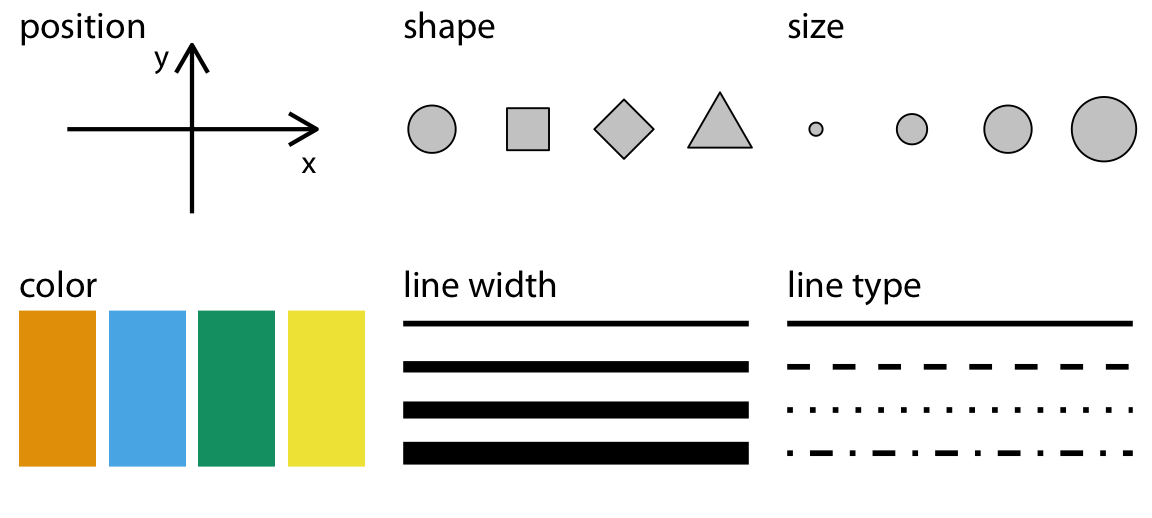
\includegraphics{images/common_aesthetics_1.png}

}

\caption{Common aesthetic attributes used in \texttt{ggplot} graphics.}

\end{figure}

Let's return to our original scatter plot (\texttt{cases} vs
\texttt{week}):

\begin{Shaded}
\begin{Highlighting}[]
\FunctionTok{ggplot}\NormalTok{(}\AttributeTok{data =}\NormalTok{ nigerm96, }
       \AttributeTok{mapping =} \FunctionTok{aes}\NormalTok{(}\AttributeTok{x =}\NormalTok{ week, }
                     \AttributeTok{y =}\NormalTok{ cases)) }\SpecialCharTok{+}
  \FunctionTok{geom\_point}\NormalTok{()}
\end{Highlighting}
\end{Shaded}

\begin{figure}[H]

{\centering \includegraphics{data_on_display_ls01_gg_intro_files/figure-pdf/unnamed-chunk-25-1.pdf}

}

\end{figure}

There are other aesthetics we can add, like color or size.

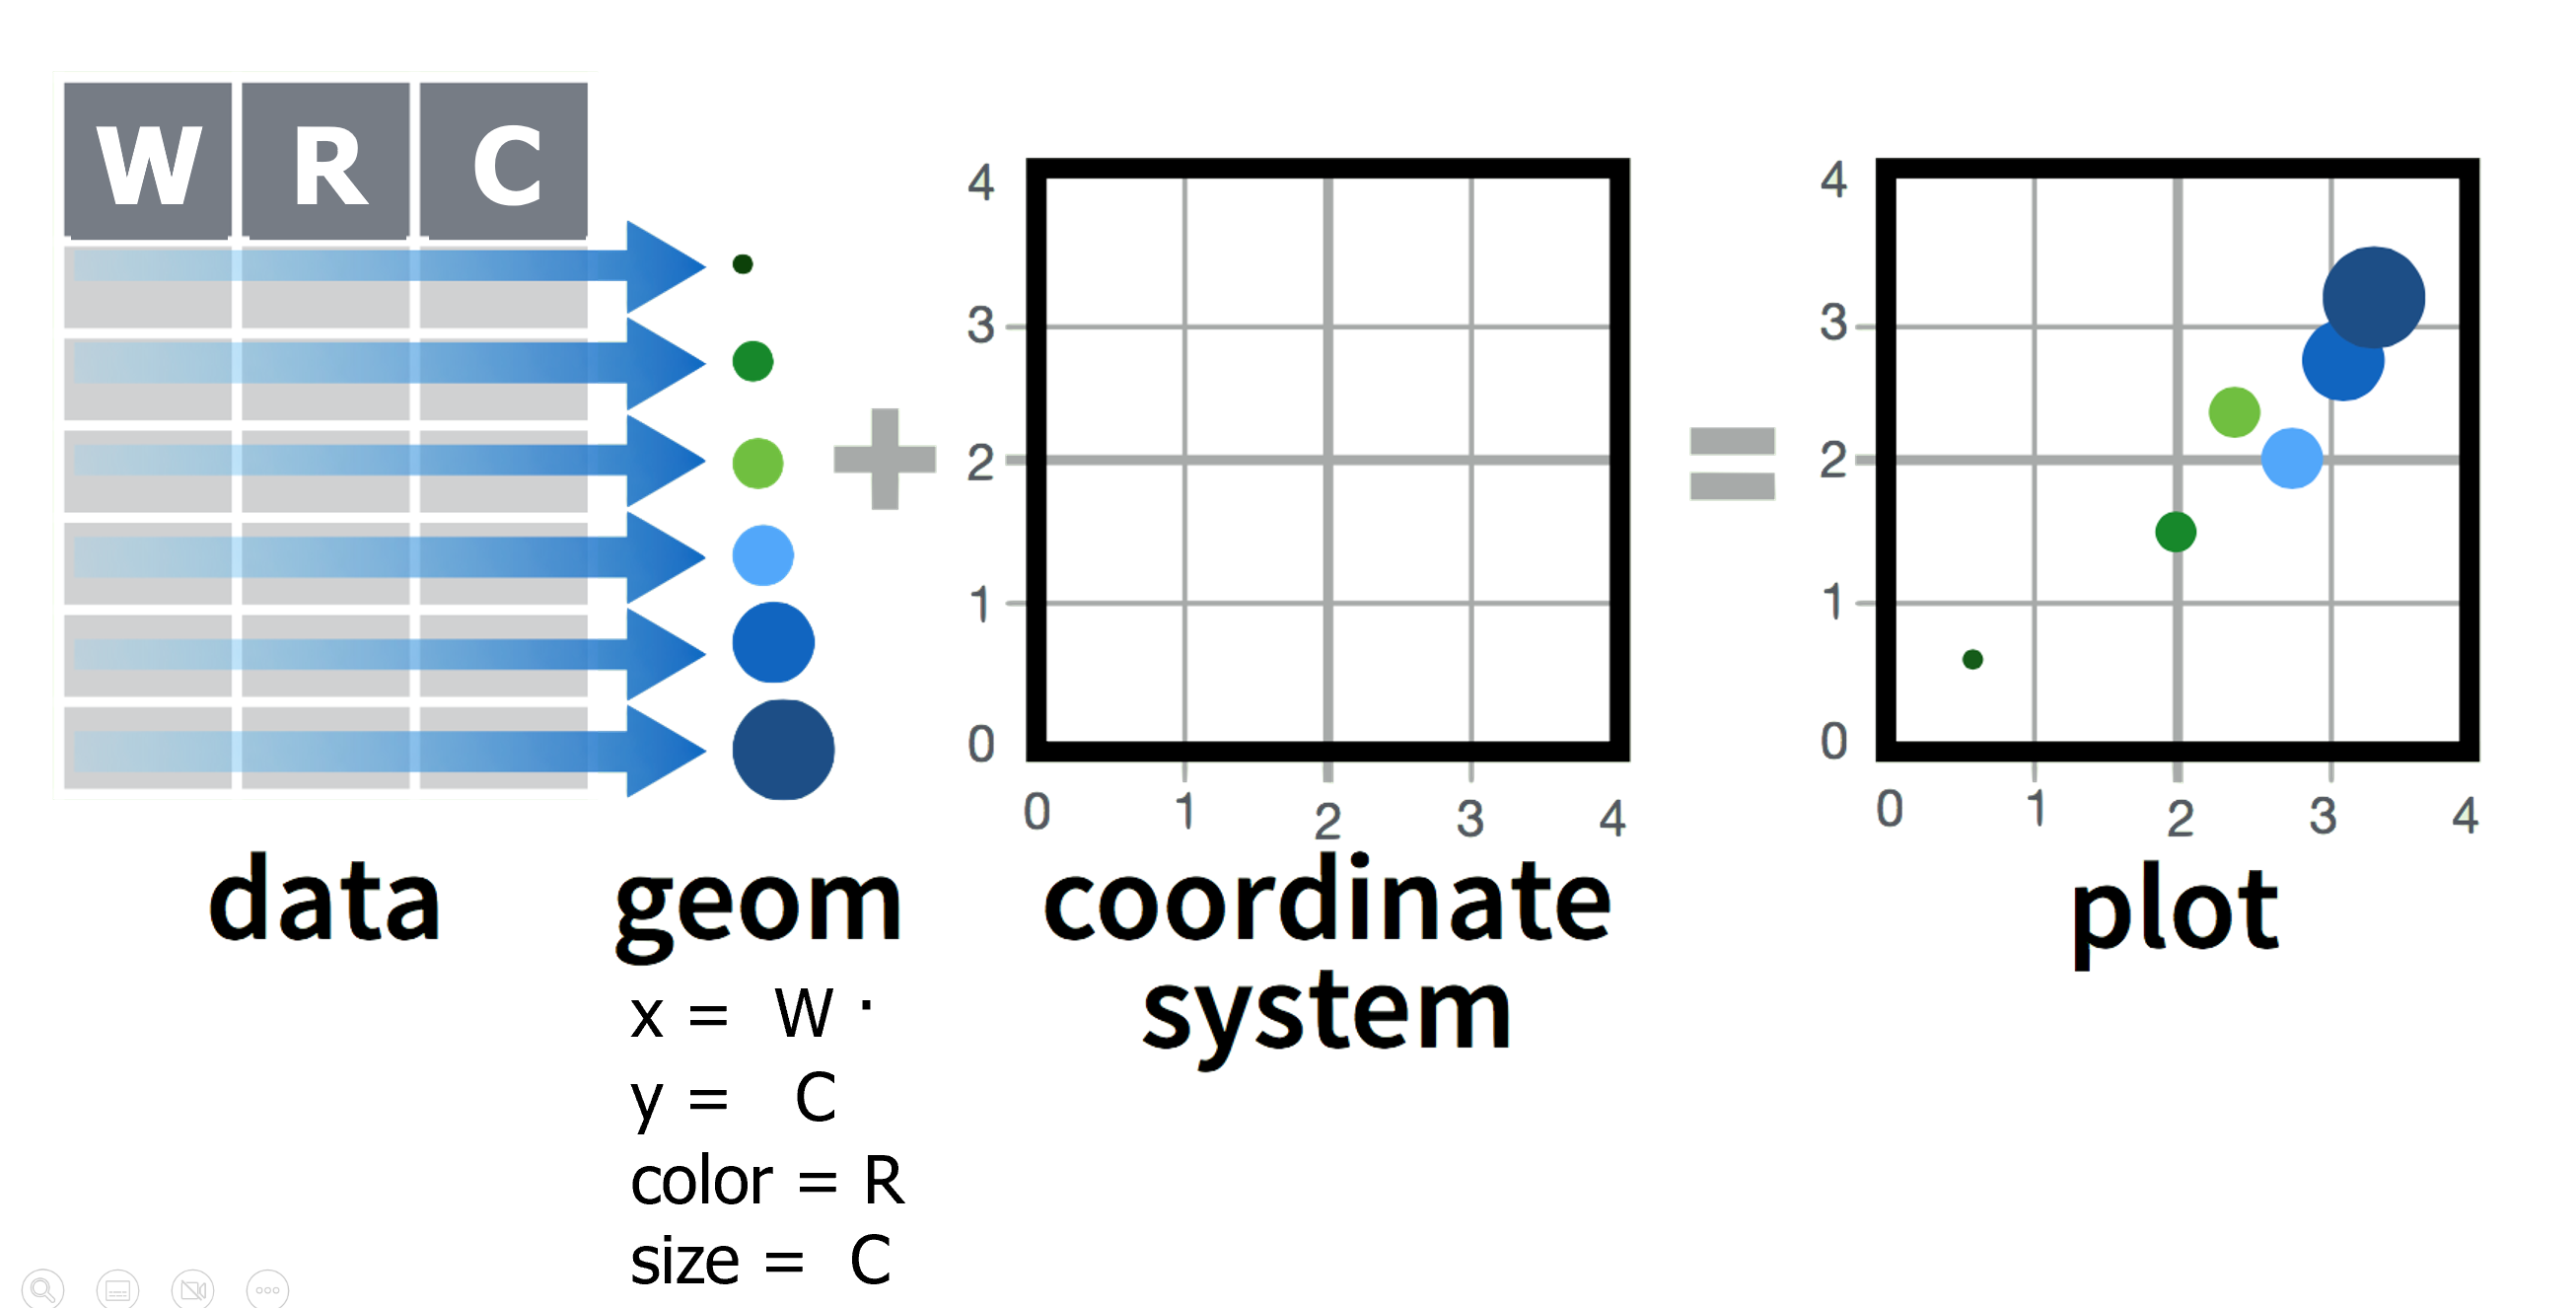
\includegraphics{images/paste-72D5BE04.png}

\begin{tcolorbox}[enhanced jigsaw, colframe=quarto-callout-note-color-frame, colbacktitle=quarto-callout-note-color!10!white, titlerule=0mm, opacitybacktitle=0.6, breakable, toprule=.15mm, arc=.35mm, rightrule=.15mm, colback=white, bottomrule=.15mm, opacityback=0, toptitle=1mm, left=2mm, bottomtitle=1mm, title=\textcolor{quarto-callout-note-color}{\faInfo}\hspace{0.5em}{Pro Tip}, leftrule=.75mm, coltitle=black]

To see the full list of aesthetics that can be used with a particular
\texttt{geom\_*} function look it up the function documentation. You can
do this by pressing F1 on a function, e.g., \texttt{geom\_point()} to
open the Help tab, and scroll down to the ``Aesthetics'' section. If F1
is hard to summon on your keyboard, type and run \texttt{?geom\_point}
in your Console tab.

\end{tcolorbox}

Let's add color to our scatter plot. We can map the categorical variable
\texttt{region} to the \texttt{color} aesthetic. We can do this by
modifying the original code to add a new argument inside
\texttt{mapping\ =\ aes()}. Let's see what happens when we add
\texttt{color\ =\ region} inside \texttt{aes()}:

\begin{Shaded}
\begin{Highlighting}[]
\FunctionTok{ggplot}\NormalTok{(}\AttributeTok{data =}\NormalTok{ nigerm96,      }
       \AttributeTok{mapping =} \FunctionTok{aes}\NormalTok{(}\AttributeTok{x =}\NormalTok{ week,  }
                     \AttributeTok{y =}\NormalTok{ cases,   }
                     \AttributeTok{color =}\NormalTok{ region)) }\SpecialCharTok{+}  \CommentTok{\# use a different color for each region}
  \FunctionTok{geom\_point}\NormalTok{()               }
\end{Highlighting}
\end{Shaded}

\begin{figure}[H]

{\centering \includegraphics{data_on_display_ls01_gg_intro_files/figure-pdf/unnamed-chunk-26-1.pdf}

}

\end{figure}

Now we have a colorful scatter plot! Each point is colored according to
the region it belongs to. This allows us to better distinguish between
regions.

Note that \texttt{ggplot()} automatically provides a color legend on the
left.

\begin{tcolorbox}[enhanced jigsaw, colframe=quarto-callout-note-color-frame, colbacktitle=quarto-callout-note-color!10!white, titlerule=0mm, opacitybacktitle=0.6, breakable, toprule=.15mm, arc=.35mm, rightrule=.15mm, colback=white, bottomrule=.15mm, opacityback=0, toptitle=1mm, left=2mm, bottomtitle=1mm, title=\textcolor{quarto-callout-note-color}{\faInfo}\hspace{0.5em}{Side Note}, leftrule=.75mm, coltitle=black]

The colors are from \{ggplot2\}'s default rainbow color palette. In
later lessons we will learn how to customize color scales and palettes,
including making figures colorblind-friendly.

\end{tcolorbox}

By examining the color patterns in the plot, you can make out the
classic bell-shaped epidemic curves showing a rise and fall in measles
incidence in each region.

Zinder had the largest number of cases and the steepest epidemic curve,
followed by Maradi and Niamey.

While the colorful plot provides more insight into measles patterns at
the regional level than the scatter plot with no color mapping, this
graph still looks busy and is not the most intuitive to read. A
different plot type could help with this.

Next we will try a bar plot, then a line graph.

Let's try the same \texttt{color\ =\ region} aesthetic mapping with
\texttt{geom\_col()} instead:

\begin{Shaded}
\begin{Highlighting}[]
\FunctionTok{ggplot}\NormalTok{(}\AttributeTok{data =}\NormalTok{ nigerm96, }
       \AttributeTok{mapping =} \FunctionTok{aes}\NormalTok{(}\AttributeTok{x =}\NormalTok{ week, }
                     \AttributeTok{y =}\NormalTok{ cases, }
                     \AttributeTok{color =}\NormalTok{ region)) }\SpecialCharTok{+}  \CommentTok{\# use a different outline color for each region}
  \FunctionTok{geom\_col}\NormalTok{()}
\end{Highlighting}
\end{Shaded}

\begin{figure}[H]

{\centering \includegraphics{data_on_display_ls01_gg_intro_files/figure-pdf/unnamed-chunk-27-1.pdf}

}

\end{figure}

This gives us a stacked bar plot, where the bars are divided into
smaller sections. This shows us the proportional contribution of
individual regions (i.e., the height or length of each subsection
represents how much each region contributes to the total number of cases
that week).

The stacked bar plot here is outlined by color. This is because the
\texttt{color} aesthetic in \{ggplot2\} generally refers to the border
around a shape. This did not apply to the default shapes in our scatter
plot created with \texttt{geom\_point()} because they are solid dots
(not hollow), but you can see that it does apply to the bars in a bar
chart created \texttt{geom\_col()}. However, the grey filling is not
very pretty.

We might want to color the inside of the bars instead. This is done by
mapping our variable to the \texttt{fill} aesthetic. We can copy the
code above and simply change \texttt{color} to \texttt{fill} inside
\texttt{aes()}:

\begin{Shaded}
\begin{Highlighting}[]
\FunctionTok{ggplot}\NormalTok{(}\AttributeTok{data =}\NormalTok{ nigerm96, }
       \AttributeTok{mapping =} \FunctionTok{aes}\NormalTok{(}\AttributeTok{x =}\NormalTok{ week, }
                     \AttributeTok{y =}\NormalTok{ cases, }
                     \AttributeTok{fill =}\NormalTok{ region)) }\SpecialCharTok{+}  \CommentTok{\# use a different fill color for each region}
  \FunctionTok{geom\_col}\NormalTok{()}
\end{Highlighting}
\end{Shaded}

\begin{figure}[H]

{\centering \includegraphics{data_on_display_ls01_gg_intro_files/figure-pdf/unnamed-chunk-28-1.pdf}

}

\end{figure}

Voila! The inside of the bars are now filled with colors.

Now practice using the \texttt{color} aesthetic mapping with a new plot
type: line graphs. Line graphs are generally considered one of the best
plot types for time series data.

\begin{tcolorbox}[enhanced jigsaw, colframe=quarto-callout-tip-color-frame, colbacktitle=quarto-callout-tip-color!10!white, titlerule=0mm, opacitybacktitle=0.6, breakable, toprule=.15mm, arc=.35mm, rightrule=.15mm, colback=white, bottomrule=.15mm, opacityback=0, toptitle=1mm, left=2mm, bottomtitle=1mm, title=\textcolor{quarto-callout-tip-color}{\faLightbulb}\hspace{0.5em}{Practice}, leftrule=.75mm, coltitle=black]

Use the \texttt{nigerm04} data frame to create a line graph of weekly
cases, colored by \texttt{region}. Map \texttt{cases} on the y-axis,
\texttt{week} on the x-axis, and \texttt{region} to color. The
\texttt{geom\_*} function for a line graph is called
\textbf{\texttt{geom\_line()}}.

\end{tcolorbox}

\hypertarget{fixed-aesthetics-outside-aes}{%
\subsection{\texorpdfstring{Fixed aesthetics outside
\texttt{aes()}}{Fixed aesthetics outside aes()}}\label{fixed-aesthetics-outside-aes}}

It is very important to understand the difference between
\textbf{aesthetic mappings} and \textbf{fixed aesthetics}. The main
aesthetics in \texttt{ggplot} are: \texttt{x}, \texttt{y},
\texttt{color}, \texttt{fill}, and \texttt{size}, and any of these could
be either a mapping or a fixed value. This depends on whether they
appear inside or outside the \texttt{aes()} function.

When we apply an aesthetic to modify the geometric objects according to
a variable (e.g., the color of points changes according to the region
variable), that's an aesthetic mapping. This must always be defined
\textbf{inside} \texttt{mapping\ =\ aes()}, like we just did in previous
examples.

But if you want to apply a visual modification to \emph{all} the
geometric objects evenly (e.g., manually change the color of all points
to be one color), that's a fixed aesthetic. We must set fixed aesthetics
to a constant value \textbf{outside} \texttt{mapping\ =\ aes()} and
directly inside the \texttt{geom\_*} function - e.g.,
\texttt{geom\_point(color\ =\ "COLOR\_NAME")}.

Here let's change the color of all the points in our scatter plot to
blue:

\begin{Shaded}
\begin{Highlighting}[]
\FunctionTok{ggplot}\NormalTok{(}\AttributeTok{data =}\NormalTok{ nigerm96, }
       \AttributeTok{mapping =} \FunctionTok{aes}\NormalTok{(}\AttributeTok{x =}\NormalTok{ week, }
                     \AttributeTok{y =}\NormalTok{ cases)) }\SpecialCharTok{+}
  \FunctionTok{geom\_point}\NormalTok{(}\AttributeTok{color =} \StringTok{"blue"}\NormalTok{)        }\CommentTok{\# use the same color for all points}
\end{Highlighting}
\end{Shaded}

\begin{figure}[H]

{\centering 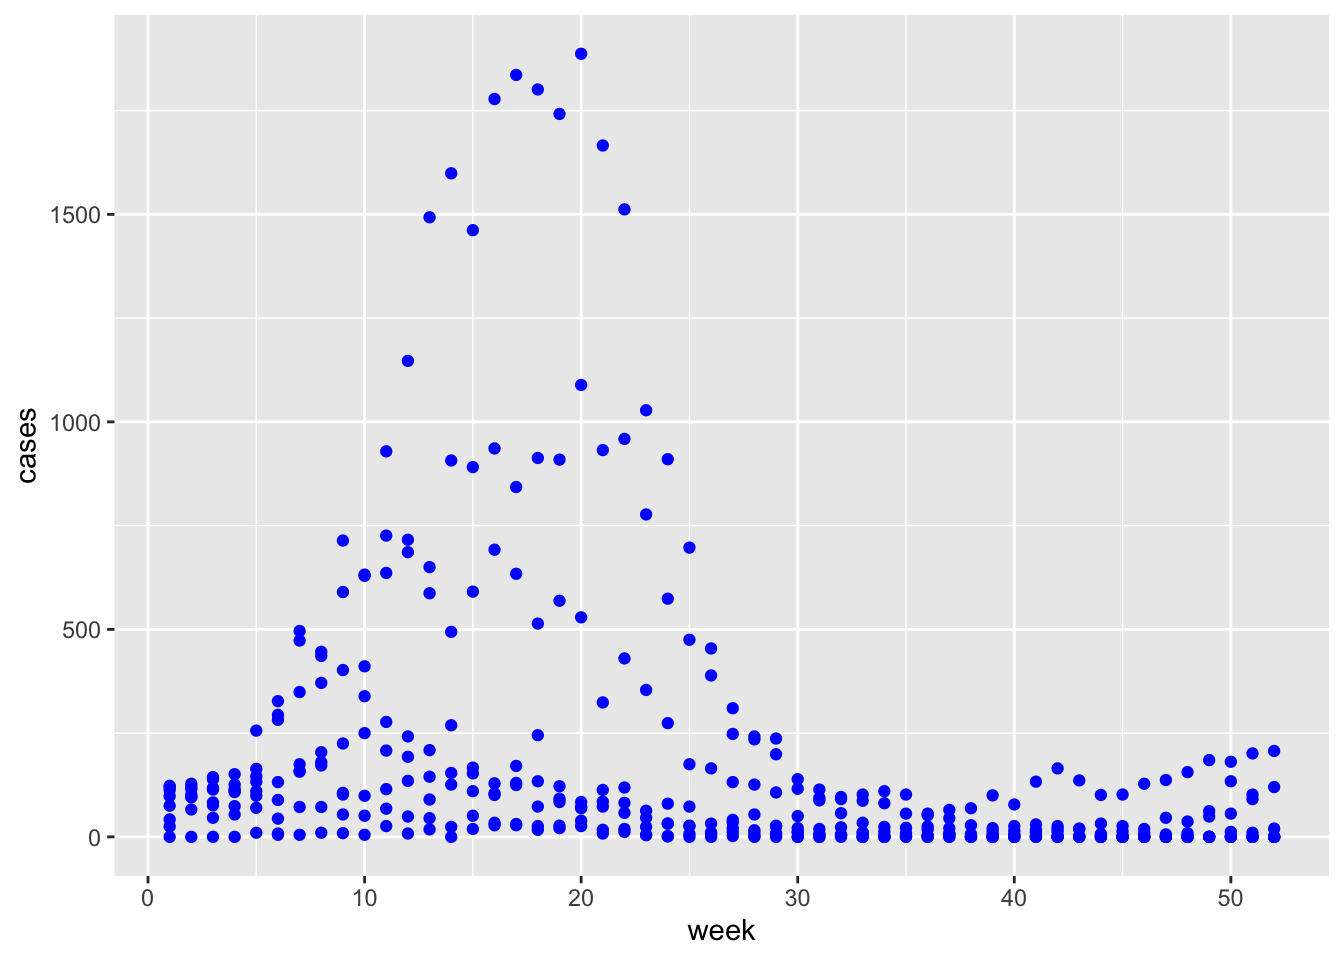
\includegraphics{data_on_display_ls01_gg_intro_files/figure-pdf/unnamed-chunk-31-1.pdf}

}

\end{figure}

This colors each point with the same R color (``blue''). In this plot,
the color aesthetic does not represent any values from the data frame.
Note that the color names in R are character strings, so it needs to go
inside quotation marks.

\begin{tcolorbox}[enhanced jigsaw, colframe=quarto-callout-note-color-frame, colbacktitle=quarto-callout-note-color!10!white, titlerule=0mm, opacitybacktitle=0.6, breakable, toprule=.15mm, arc=.35mm, rightrule=.15mm, colback=white, bottomrule=.15mm, opacityback=0, toptitle=1mm, left=2mm, bottomtitle=1mm, title=\textcolor{quarto-callout-note-color}{\faInfo}\hspace{0.5em}{Side Note}, leftrule=.75mm, coltitle=black]

If you're curious, run \texttt{colors()} in your console to see all
possible choice of colors in R! To find out exactly how many options
that is, try running \texttt{colors()\ \%\textgreater{}\%\ length()}.

\end{tcolorbox}

Now let's add a fixed aesthetic called \texttt{size}. The default line
width used by \texttt{geom\_line()} is 0.5 mm, which looks like this:

\begin{Shaded}
\begin{Highlighting}[]
\FunctionTok{ggplot}\NormalTok{(}\AttributeTok{data =}\NormalTok{ nigerm96, }
             \AttributeTok{mapping =} \FunctionTok{aes}\NormalTok{(}\AttributeTok{x =}\NormalTok{ week, }
                           \AttributeTok{y =}\NormalTok{ cases,}
                           \AttributeTok{color =}\NormalTok{ region)) }\SpecialCharTok{+} 
      \FunctionTok{geom\_line}\NormalTok{()}
\end{Highlighting}
\end{Shaded}

\begin{figure}[H]

{\centering 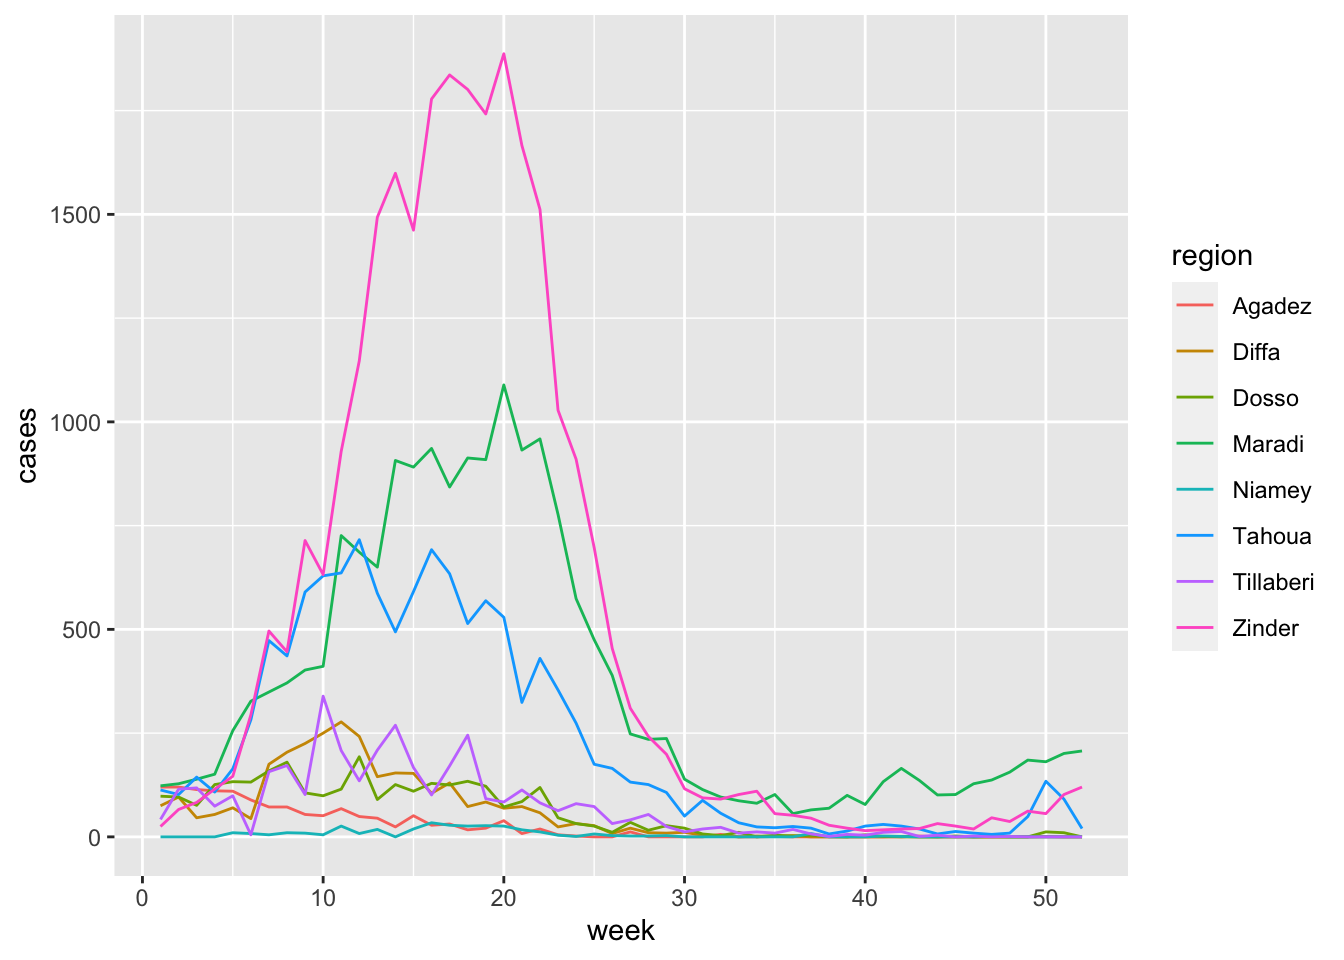
\includegraphics{data_on_display_ls01_gg_intro_files/figure-pdf/unnamed-chunk-32-1.pdf}

}

\end{figure}

To make all of the lines in our figure a little thicker, let's fix this
aesthetic at 1 mm. We do this by adding \texttt{size\ =\ 1} inside the
\texttt{geom\_line()} function:

\begin{Shaded}
\begin{Highlighting}[]
\FunctionTok{ggplot}\NormalTok{(}\AttributeTok{data =}\NormalTok{ nigerm96, }
             \AttributeTok{mapping =} \FunctionTok{aes}\NormalTok{(}\AttributeTok{x =}\NormalTok{ week, }
                           \AttributeTok{y =}\NormalTok{ cases,}
                           \AttributeTok{color =}\NormalTok{ region)) }\SpecialCharTok{+} 
      \FunctionTok{geom\_line}\NormalTok{(}\AttributeTok{size =} \DecValTok{1}\NormalTok{)}
\end{Highlighting}
\end{Shaded}

\begin{verbatim}
Warning: Using `size` aesthetic for lines was deprecated in ggplot2 3.4.0.
i Please use `linewidth` instead.
\end{verbatim}

\begin{figure}[H]

{\centering 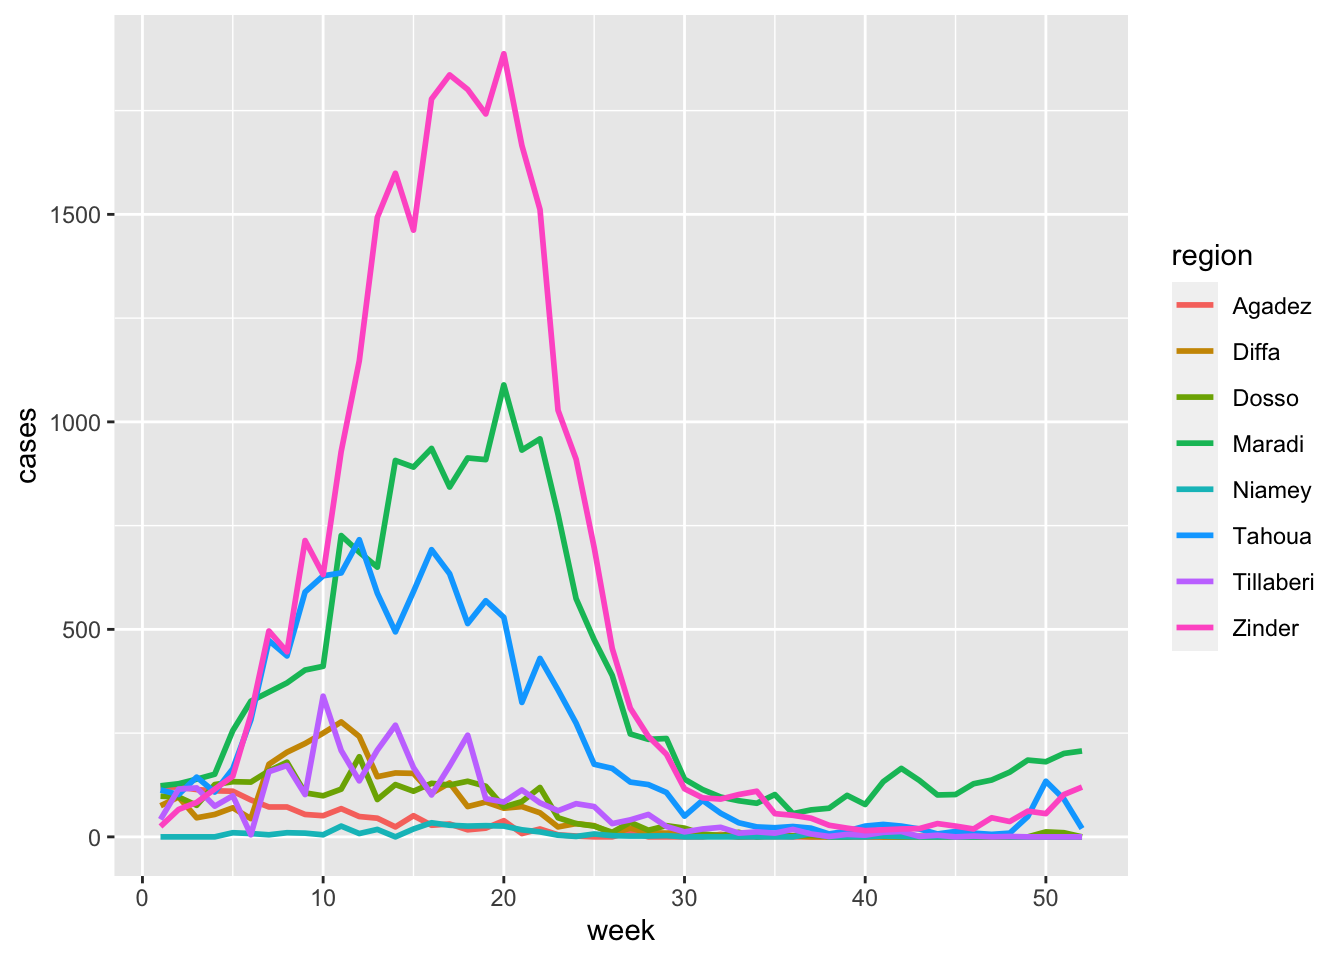
\includegraphics{data_on_display_ls01_gg_intro_files/figure-pdf/unnamed-chunk-33-1.pdf}

}

\end{figure}

All the lines in the plot have been made thicker, and the line width is
set to a constant value of 1 mm. Note that here the value of size is
numeric, so it should not be in quotation marks.

\begin{tcolorbox}[enhanced jigsaw, colframe=quarto-callout-caution-color-frame, colbacktitle=quarto-callout-caution-color!10!white, titlerule=0mm, opacitybacktitle=0.6, breakable, toprule=.15mm, arc=.35mm, rightrule=.15mm, colback=white, bottomrule=.15mm, opacityback=0, toptitle=1mm, left=2mm, bottomtitle=1mm, title=\textcolor{quarto-callout-caution-color}{\faFire}\hspace{0.5em}{Watch Out}, leftrule=.75mm, coltitle=black]

Remember that fixed aesthetics are manually set to constant value (as
opposed to a variable from the data), and goes directly in the
\texttt{geom\_*} function, \textbf{not} inside \texttt{aes()}. If you
try to put a fixed aesthetic in \texttt{aes()}, you might get a weird
result. For example, let's try moving the \texttt{size\ =\ 1} aesthetic
from \texttt{geom\_line()} to \texttt{aes()} to see how it can go wrong:

\begin{Shaded}
\begin{Highlighting}[]
\FunctionTok{ggplot}\NormalTok{(}\AttributeTok{data =}\NormalTok{ nigerm96, }
             \AttributeTok{mapping =} \FunctionTok{aes}\NormalTok{(}\AttributeTok{x =}\NormalTok{ week, }
                           \AttributeTok{y =}\NormalTok{ cases,}
                           \AttributeTok{color =}\NormalTok{ region,}
                           \AttributeTok{size =} \DecValTok{1}\NormalTok{)) }\SpecialCharTok{+}     \CommentTok{\# INCORRECT placement}
      \FunctionTok{geom\_line}\NormalTok{()}
\end{Highlighting}
\end{Shaded}

\begin{figure}[H]

{\centering 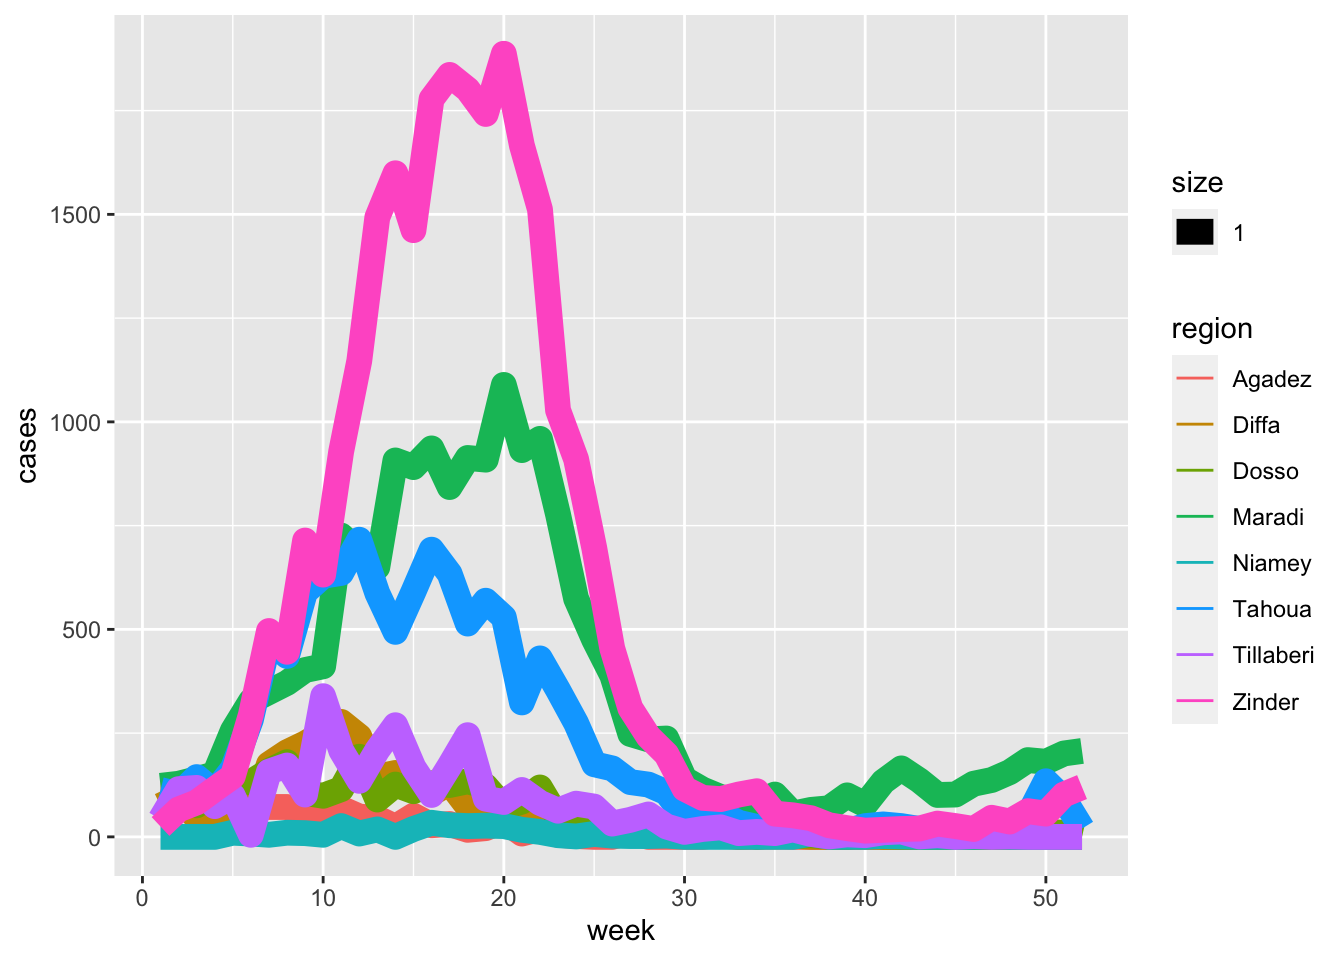
\includegraphics{data_on_display_ls01_gg_intro_files/figure-pdf/unnamed-chunk-34-1.pdf}

}

\end{figure}

\texttt{aes()} is a mapping function that modifies plots based on
variables from the data. Since there is no variable called ``1'' in the
\texttt{nigerm96} data frame, \texttt{aes()} cannot process or map this
aesthetic correctly.

\end{tcolorbox}

Practice using \texttt{fill} as a fixed aesthetic for a bar plot.

\begin{tcolorbox}[enhanced jigsaw, colframe=quarto-callout-tip-color-frame, colbacktitle=quarto-callout-tip-color!10!white, titlerule=0mm, opacitybacktitle=0.6, breakable, toprule=.15mm, arc=.35mm, rightrule=.15mm, colback=white, bottomrule=.15mm, opacityback=0, toptitle=1mm, left=2mm, bottomtitle=1mm, title=\textcolor{quarto-callout-tip-color}{\faLightbulb}\hspace{0.5em}{Practice}, leftrule=.75mm, coltitle=black]

Use the \texttt{nigerm04} data frame to create a bar graph of weekly
cases, and fill all bars with the same color. Map \texttt{cases} on the
y-axis, \texttt{week} on the x-axis, and fix the \texttt{color}
aesthetic of the bars to the R color ``hotpink''.

\end{tcolorbox}

\hypertarget{additional-gg-layers}{%
\section{Additional GG layers}\label{additional-gg-layers}}

In this lesson, we kept things simple and only worked with the three
required layers. As you start to delve deeper into plotting with
\{ggplot2\}, you'll start to encounter the other layers more frequently.

Soon you'll be able to create more complex plots, like this one:

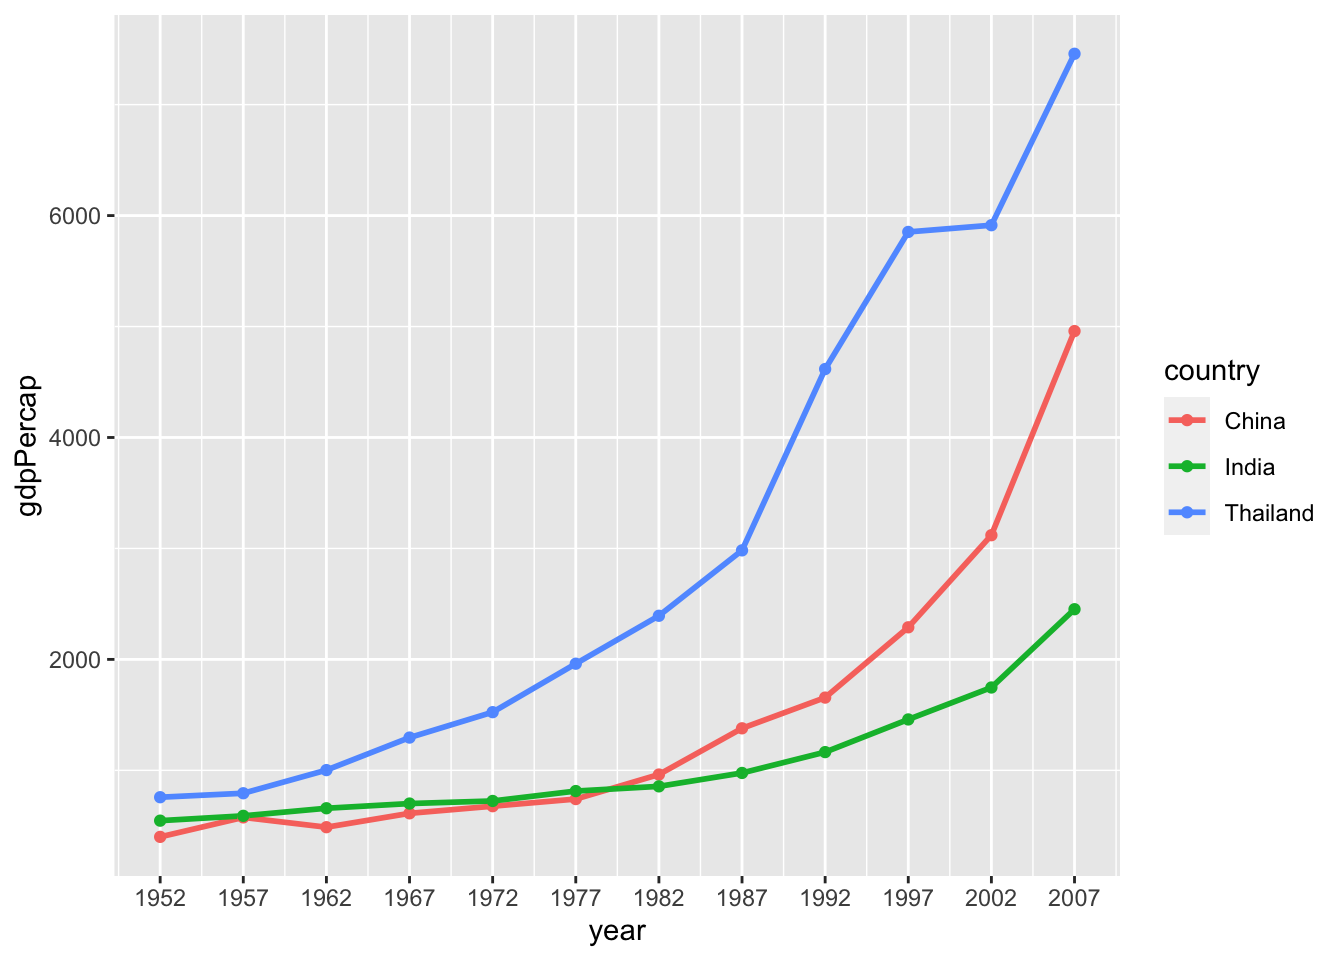
\includegraphics{data_on_display_ls01_gg_intro_files/figure-pdf/unnamed-chunk-37-1.pdf}

\begin{tcolorbox}[enhanced jigsaw, colframe=quarto-callout-note-color-frame, colbacktitle=quarto-callout-note-color!10!white, titlerule=0mm, opacitybacktitle=0.6, breakable, toprule=.15mm, arc=.35mm, rightrule=.15mm, colback=white, bottomrule=.15mm, opacityback=0, toptitle=1mm, left=2mm, bottomtitle=1mm, title=\textcolor{quarto-callout-note-color}{\faInfo}\hspace{0.5em}{Recap}, leftrule=.75mm, coltitle=black]

To build a complete \texttt{ggplot}, you must first supply a data frame
using the \textbf{\texttt{data}} argument of \texttt{ggplot()}, and
define variables and map them to aesthetics inside \texttt{aes()} using
the \textbf{\texttt{mapping}} argument of \texttt{ggplot()}. Then start
a new layer with a \textbf{\texttt{+}} sign and specify the type of plot
you want using an appropriate \textbf{\texttt{geom\_*}} function. You
can copy this code template and adapt it to create different
\texttt{ggplot} graphics:

\begin{Shaded}
\begin{Highlighting}[]
\FunctionTok{ggplot}\NormalTok{(}\AttributeTok{data =}\NormalTok{ DF\_NAME,}
       \AttributeTok{mapping =} \FunctionTok{aes}\NormalTok{(}\AttributeTok{AES1 =}\NormalTok{ VAR1,}
                     \AttributeTok{AES2 =}\NormalTok{ VAR2, }
                     \AttributeTok{AES3 =}\NormalTok{ VAR3, }
\NormalTok{                     ...)) }\SpecialCharTok{+}
  \FunctionTok{geom\_FUCNTION}\NormalTok{()}
\end{Highlighting}
\end{Shaded}

\end{tcolorbox}

\hypertarget{learning-outcomes}{%
\section{Learning outcomes}\label{learning-outcomes}}

\begin{enumerate}
\def\labelenumi{\arabic{enumi}.}
\item
  You can recall and explain how the \textbf{\{ggplot2\}} package for
  data visualization is based on a theoretical framework called the
  \textbf{grammar of graphics}.
\item
  You can name and describe the 3 essential layers for building a graph:
  \textbf{data}, \textbf{aesthetics}, and \textbf{geometries}.
\item
  You can write code to \textbf{build a complete \texttt{ggplot}}
  \textbf{graphic} by correctly supplying the 3 essential layers to the
  \textbf{\texttt{ggplot()}} \textbf{function}.
\item
  You can create different types of plots such as \textbf{scatter
  plots}, \textbf{line graphs}, and \textbf{bar graphs}.
\item
  You can add or modify aesthetics of a plot such as the \textbf{color},
  and \textbf{size}.
\end{enumerate}

The following team members contributed to this lesson:

\hypertarget{references}{%
\section*{References}\label{references}}

\markright{References}

Some material in this lesson was adapted from the following sources:

\begin{itemize}
\item
  Blake, Alexandre, Ali Djibo, Ousmane Guindo, and Nita Bharti. 2020.
  ``Investigating Persistent Measles Dynamics in Niger and Associations
  with Rainfall.'' \emph{Journal of The Royal Society Interface} 17
  (169): 20200480. \url{https://doi.org/10.1098/rsif.2020.0480}.
\item
  Cmprince.~\emph{Administrative divisions of Niger: Departments and
  Regions}. 29 October 2017. Wikimedia Commons. Accessed October 14,
  2022.
  \url{https://commons.wikimedia.org/wiki/File:Niger_administrative_divisions.svg}
\item
  DeBruine, Lisa, and Dale Barr. 2022. \emph{Chapter 3 Data
  Visualisation \textbar{} Data Skills for Reproducible Research}.
  \url{https://psyteachr.github.io/reprores-v3/ggplot.html}.
\item
  Franke, Michael. n.d. \emph{6 Data Visualization \textbar{} An
  Introduction to Data Analysis}. Accessed October 12, 2022.
  \url{https://michael-franke.github.io/intro-data-analysis/Chap-02-02-visualization.html}.
\item
  Geography Now, dir. 2019. \emph{Geography Now! NIGER}.
  \url{https://www.youtube.com/watch?v=AHeq99pojLo}.
\item
  Giroux-Bougard, Xavier, Maxwell Farrell, Amanda Winegardner, Étienne
  Low-Decarie and Monica Granados. 2020. \emph{Workshop 3: Introduction
  to Data Visualisation with Ggplot2}.
  \url{http://r.qcbs.ca/workshop03/book-en/}.
\item
  Ismay, Chester, and Albert Y. Kim. 2022. \emph{A ModernDive into R and
  the Tidyverse}. \url{https://moderndive.com/}.
\item
  Kabacoff, Rob. 2020. \emph{Data Visualization with R}.
  \url{https://rkabacoff.github.io/datavis/}.
\item
  Lisa DeBruine. 2020. \emph{Basic Plots}.
  \url{https://www.youtube.com/watch?v=tOFQFPRgZ3M}.
\item
  Pius, Ewen Harrison and Riinu. n.d. \emph{R for Health Data Science}.
  Accessed October 11, 2022.
  \url{https://argoshare.is.ed.ac.uk/healthyr_book/}.
\item
  Prabhakaran, Selva. 2016. ``How to Make Any Plot in Ggplot2?
  \textbar{} Ggplot2 Tutorial.'' 2016.
  \url{http://r-statistics.co/ggplot2-Tutorial-With-R.html}.
\end{itemize}

\hypertarget{solutions}{%
\section{Solutions}\label{solutions}}

\begin{Shaded}
\begin{Highlighting}[]
\FunctionTok{.SOLUTION\_nigerm04\_scatter}\NormalTok{()}
\end{Highlighting}
\end{Shaded}

\begin{verbatim}
ggplot(data = nigerm04,
             mapping = aes(x = week, 
                           y = cases)) +
      geom_point()
\end{verbatim}

\begin{Shaded}
\begin{Highlighting}[]
\FunctionTok{.SOLUTION\_nigerm04\_bar}\NormalTok{()}
\end{Highlighting}
\end{Shaded}

\begin{verbatim}
ggplot(data = nigerm04, 
          mapping = aes(x = week, 
                        y = cases)) + 
     geom_col()
\end{verbatim}

\begin{Shaded}
\begin{Highlighting}[]
\FunctionTok{.SOLUTION\_nigerm04\_line}\NormalTok{()}
\end{Highlighting}
\end{Shaded}

\begin{verbatim}
ggplot(data = nigerm04,
         mapping = aes(x = week,
                       y = cases,
                       color = region)) + 
    geom_line()
\end{verbatim}

\begin{Shaded}
\begin{Highlighting}[]
\FunctionTok{.SOLUTION\_nigerm04\_pinkbar}\NormalTok{()}
\end{Highlighting}
\end{Shaded}

\begin{verbatim}
ggplot(data = nigerm04, 
          mapping = aes(x = week, 
                        y = cases)) +
      geom_col(fill = "hotpink")
\end{verbatim}

\bookmarksetup{startatroot}

\hypertarget{scatter-plots-and-smoothing-lines}{%
\chapter{Scatter plots and smoothing
lines}\label{scatter-plots-and-smoothing-lines}}

\hypertarget{introduction-1}{%
\section{Introduction}\label{introduction-1}}

\textbf{Scatter plots} - which are sometimes called \textbf{bivariate
plots} - allow you to visualize the \textbf{relationship} between two
numerical variables.

They are among the most commonly used plots because they can provide an
immediate way to see how one numerical variable varies against another.

Scatter plots can also display multiple relationships by mapping
additional variable to aesthetic properties, such as color of the
points.

Trends and relationships in a scatter plot can be made clearer by adding
a smoothing line over the points.

We will use ggplot to do all that and more. Let's get started!

\hypertarget{learning-objectives-1}{%
\section{Learning Objectives}\label{learning-objectives-1}}

\begin{enumerate}
\def\labelenumi{\arabic{enumi}.}
\tightlist
\item
  You can visualize relationships between numerical variables using
  \textbf{scatter plots} with \textbf{\texttt{geom\_point()}}.
\item
  You can use \textbf{\texttt{color}} as an aesthetic argument to map
  variables from the dataset onto individual points.
\item
  You can change the size, shape, color, fill, and opacity of geometric
  objects by setting \textbf{fixed aesthetics}.
\item
  You can add a \textbf{trend line} to a scatter plot with
  \textbf{\texttt{geom\_smooth()}}.
\end{enumerate}

\hypertarget{childhood-diarrheal-diseases-in-mali}{%
\section{Childhood diarrheal diseases in
Mali}\label{childhood-diarrheal-diseases-in-mali}}

We will be using data collected for a prospective observational study of
acute \textbf{diarrhea in children} aged 0-59 months. The study was
conducted in Mali and in early 2020.

The full dataset can be obtained from
\href{https://doi.org/10.5061/dryad.0rxwdbs19}{Dryad}, and the paper can
be viewed \href{https://elifesciences.org/articles/72294}{here}.

\begin{tcolorbox}[enhanced jigsaw, colframe=quarto-callout-note-color-frame, colbacktitle=quarto-callout-note-color!10!white, titlerule=0mm, opacitybacktitle=0.6, breakable, toprule=.15mm, arc=.35mm, rightrule=.15mm, colback=white, bottomrule=.15mm, opacityback=0, toptitle=1mm, left=2mm, bottomtitle=1mm, title=\textcolor{quarto-callout-note-color}{\faInfo}\hspace{0.5em}{Vocab}, leftrule=.75mm, coltitle=black]

A prospective study watches for outcomes, such as the development of a
disease, during the study period and relates this to other factors such
as suspected risk or protection factors.

\end{tcolorbox}

Spend some time browsing through this dataset. Each row corresponds to
one patient surveyed. There are demographic, physiological, clinical,
socioeconomic, and geographic variables.

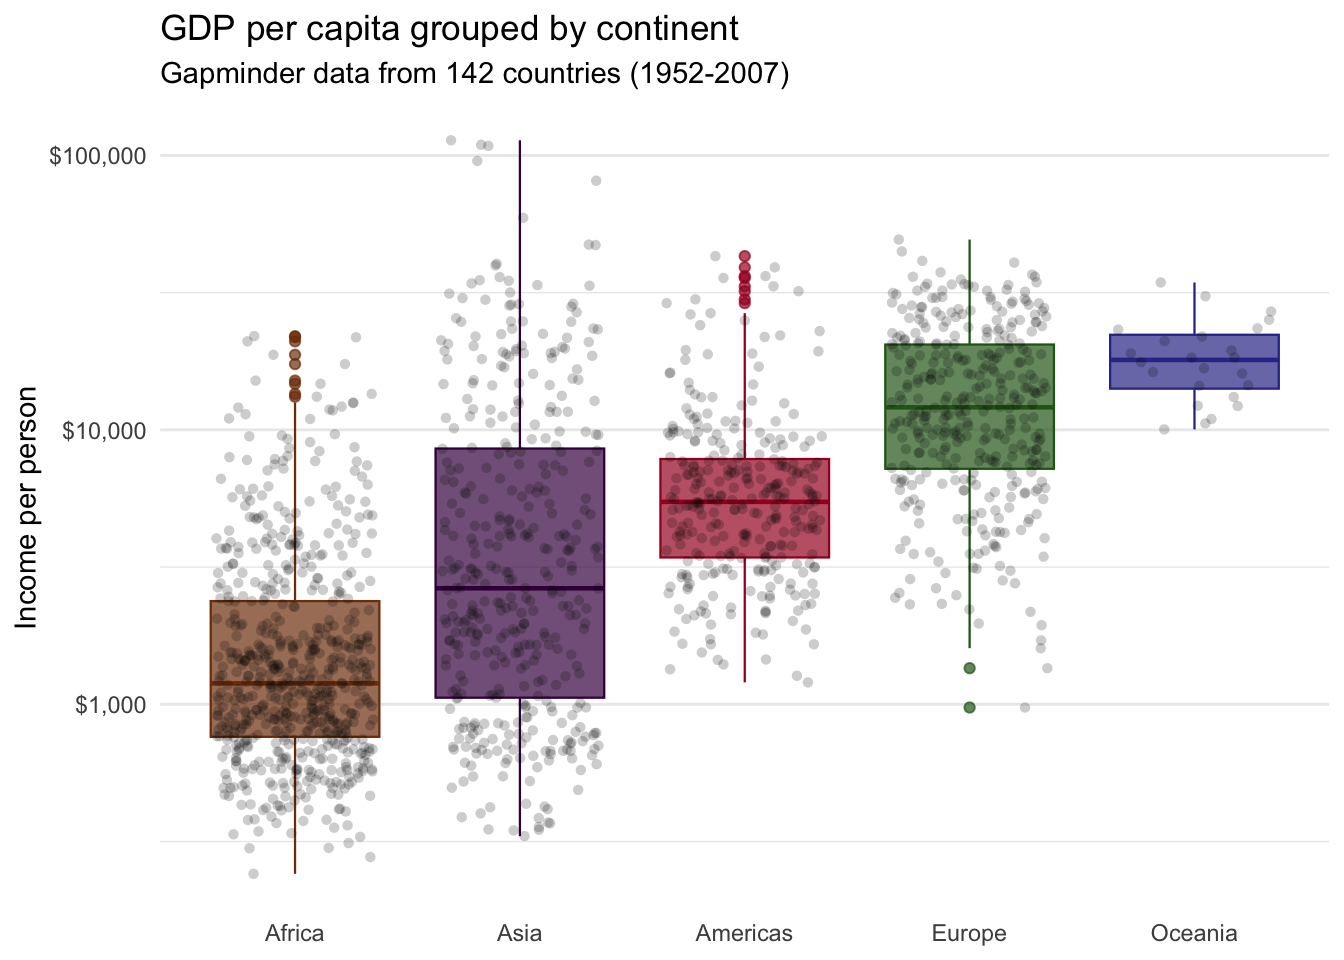
\includegraphics{data_on_display_ls02_scatter_files/figure-pdf/unnamed-chunk-3-1.pdf}

We will begin by visualizing the relationship between the following two
numerical variables:

\begin{enumerate}
\def\labelenumi{\arabic{enumi}.}
\tightlist
\item
  \texttt{age\_months}: the patient's \textbf{age} in months on the
  horizontal \textbf{x}-axis and
\item
  \texttt{viral\_load}: the patient's \textbf{viral load} on the
  vertical \textbf{y}-axis
\end{enumerate}

\hypertarget{scatter-plots-via-geom_point}{%
\section{\texorpdfstring{Scatter plots via
\texttt{geom\_point()}}{Scatter plots via geom\_point()}}\label{scatter-plots-via-geom_point}}

We will explore relationships between some numerical variables in the
\textbf{\texttt{malidd}} data frame.

We will now examine at and run the code that will create the desired
scatter plot, while keeping in mind the GG framework. Let's take a look
at the code and break it down piece-by-piece.

Remember that we specify the first two GG layers as arguments (i.e.,
inputs) within the \texttt{ggplot()} function:

\begin{enumerate}
\def\labelenumi{\arabic{enumi}.}
\tightlist
\item
  We provide the \texttt{malidd} data frame with the
  \textbf{\texttt{data}} argument, by inputting
  \textbf{\texttt{data\ =\ malidd}}.
\item
  We define the variables to be plotted in the \texttt{aes}thetics
  function of the \textbf{\texttt{mapping}} argument, by inputting
  \textbf{\texttt{mapping\ =\ aes(x\ =\ age\_months,\ y\ =\ viral\_load)}}.
  Specifically, the variable \texttt{age\_months} is mapped to the
  \texttt{x} aesthetic, while the variable \texttt{viral\_load} is
  mapped to the \texttt{y} aesthetic.
\end{enumerate}

We then add \textbf{the \texttt{geom\_*()} function} on a new layer with
a \textbf{\texttt{+}} sign. The geometric objects (i.e., shapes) needed
for a scatter plot are points, so we add
\textbf{\texttt{geom\_point()}}.

After running the following lines of code, you'll produce the scatter
plot below:

\begin{Shaded}
\begin{Highlighting}[]
\DocumentationTok{\#\# Simple scatter plot of viral load vs age}
\FunctionTok{ggplot}\NormalTok{(}\AttributeTok{data =}\NormalTok{ malidd, }
       \AttributeTok{mapping =} \FunctionTok{aes}\NormalTok{(}\AttributeTok{x =}\NormalTok{ age\_months, }
                     \AttributeTok{y =}\NormalTok{ viral\_load)) }\SpecialCharTok{+} 
  \FunctionTok{geom\_point}\NormalTok{()}
\end{Highlighting}
\end{Shaded}

\begin{figure}[H]

{\centering 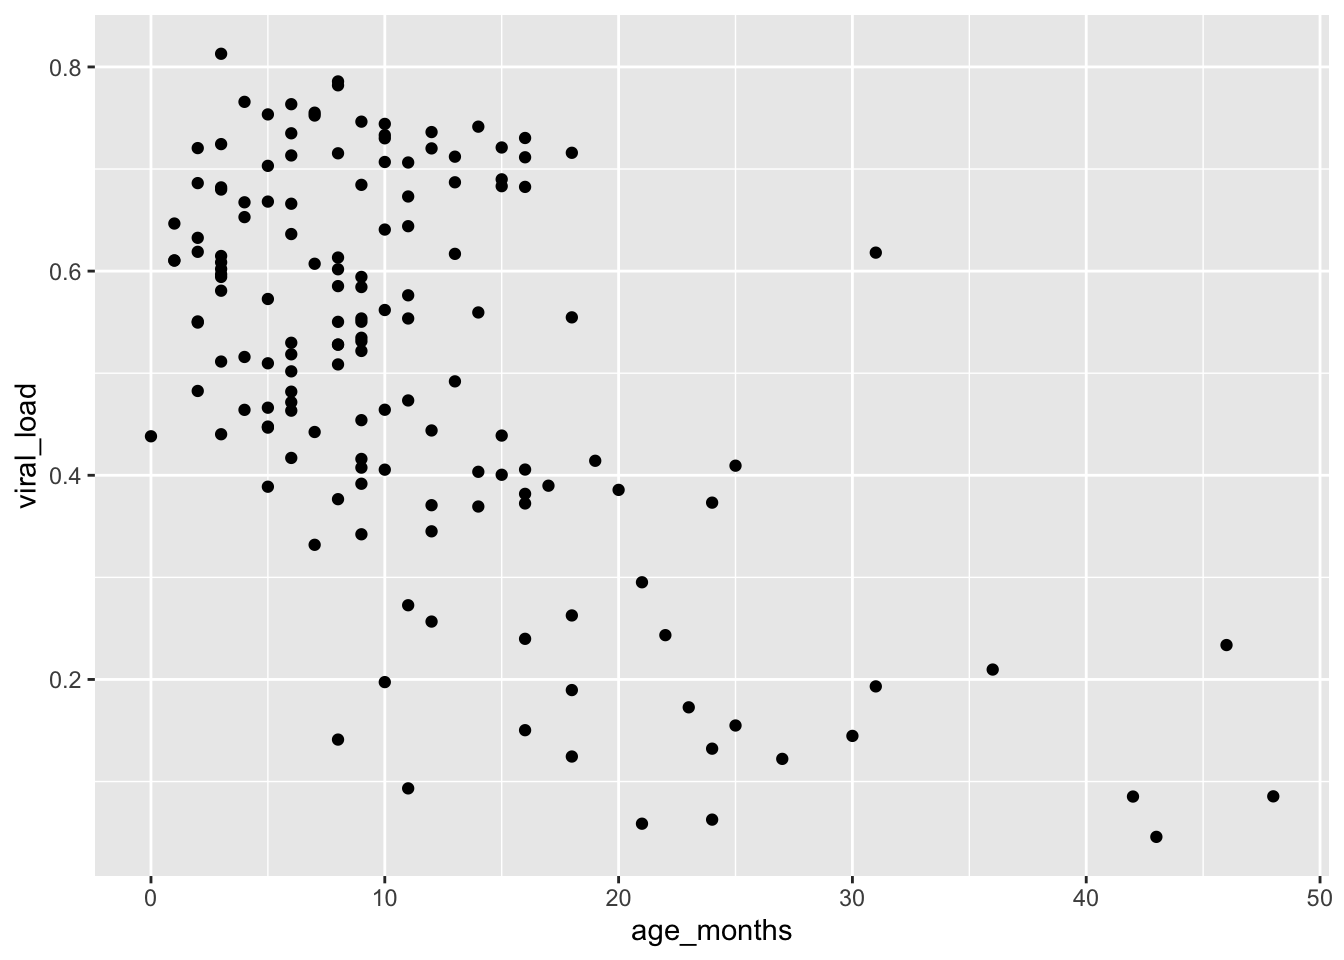
\includegraphics{data_on_display_ls02_scatter_files/figure-pdf/unnamed-chunk-4-1.pdf}

}

\end{figure}

This suggests that viral load generally \textbf{decreases} with age.

\begin{tcolorbox}[enhanced jigsaw, colframe=quarto-callout-tip-color-frame, colbacktitle=quarto-callout-tip-color!10!white, titlerule=0mm, opacitybacktitle=0.6, breakable, toprule=.15mm, arc=.35mm, rightrule=.15mm, colback=white, bottomrule=.15mm, opacityback=0, toptitle=1mm, left=2mm, bottomtitle=1mm, title=\textcolor{quarto-callout-tip-color}{\faLightbulb}\hspace{0.5em}{Practice}, leftrule=.75mm, coltitle=black]

\begin{itemize}
\tightlist
\item
  Using the \texttt{malidd} data frame, create a scatter plot showing
  the relationship between age and height (\texttt{height\_cm}).
\end{itemize}

\end{tcolorbox}

\hypertarget{aesthetic-modifications}{%
\section{Aesthetic modifications}\label{aesthetic-modifications}}

An aesthetic is a visual property of the geometric objects
(\texttt{geom}s) in your plot. Aesthetics include things like the size,
the shape, or the color of your points. You can display a point in
different ways by changing the values of its aesthetic properties.

Remember, there are two methods for changing the aesthetic properties of
your \texttt{geom}s (in this case, points).

\begin{enumerate}
\def\labelenumi{\arabic{enumi}.}
\item
  You can convey information about your data by \emph{mapping} the
  variables in your dataset to aesthetics in your plot. For this method,
  you use \texttt{aes()} in the \texttt{mapping} argument to associate
  the name of the aesthetic with a variable to display.
\item
  You can also \emph{set} the aesthetic properties of your
  \texttt{geom}s \emph{manually}. Here the aesthetic doesn't convey
  information about a variable, but only changes the appearance of the
  plot. To change an aesthetic manually, you set the aesthetic by name
  as an argument of your \texttt{geom\_*()} function; i.e.~it goes
  \emph{outside} of \texttt{aes()}.
\end{enumerate}

\hypertarget{mapping-data-to-aesthetics}{%
\subsection{Mapping data to
aesthetics}\label{mapping-data-to-aesthetics}}

In addition to mapping variables to the \textbf{x} and \textbf{y} axes
like with did above, variables can be mapped to the color, shape, size,
opacity, and other visual characteristics of \texttt{geom}s. This allows
groups of observations to be superimposed in a single graph.

To map a variable to an aesthetic, associate the name of the aesthetic
to the name of the variable inside \texttt{aes()}. This way, we can
visualize a third variable to our simple two dimensional scatter plot by
mapping it to a new aesthetic.

For example, let's map \texttt{height\_cm} to the colors of our points,
to show us how height varies with age and viral load:

\begin{Shaded}
\begin{Highlighting}[]
\FunctionTok{ggplot}\NormalTok{(}\AttributeTok{data =}\NormalTok{ malidd, }
       \AttributeTok{mapping =} \FunctionTok{aes}\NormalTok{(}\AttributeTok{x =}\NormalTok{ age\_months, }
                     \AttributeTok{y =}\NormalTok{ viral\_load)) }\SpecialCharTok{+} 
  \FunctionTok{geom\_point}\NormalTok{(}\AttributeTok{mapping =} \FunctionTok{aes}\NormalTok{(}\AttributeTok{color =}\NormalTok{ height\_cm))}
\end{Highlighting}
\end{Shaded}

\begin{figure}[H]

{\centering 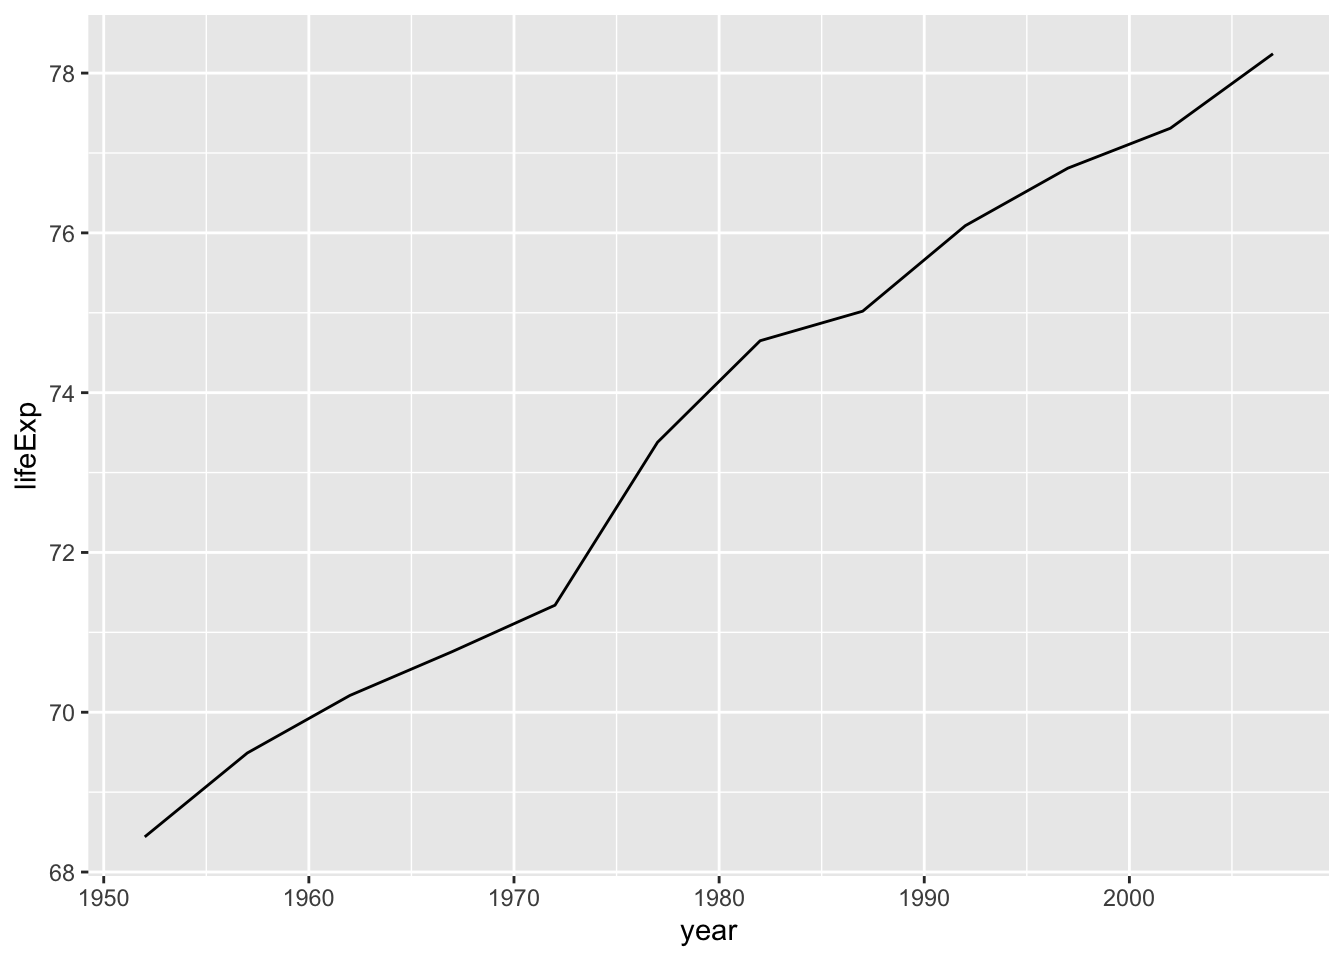
\includegraphics{data_on_display_ls02_scatter_files/figure-pdf/unnamed-chunk-7-1.pdf}

}

\end{figure}

We see that \{ggplot2\} has automatically assigned the values of our
variable to an aesthetic, a process known as \textbf{scaling}.
\{ggplot2\} will also add a legend that explains which levels correspond
to which values.

Here the points are colored by different shades of the same blue hue,
with darker colors representing lower values.

This shows us that height increases with age, as expected.

Instead of a continuous variable like \texttt{height\_cm}, we can also
map a binary variable like \texttt{breastfeeding}, to show us the which
children are breastfed and which ones are not:

\begin{Shaded}
\begin{Highlighting}[]
\FunctionTok{ggplot}\NormalTok{(}\AttributeTok{data =}\NormalTok{ malidd, }
       \AttributeTok{mapping =} \FunctionTok{aes}\NormalTok{(}\AttributeTok{x =}\NormalTok{ age\_months, }
                     \AttributeTok{y =}\NormalTok{ viral\_load)) }\SpecialCharTok{+} 
  \FunctionTok{geom\_point}\NormalTok{(}\AttributeTok{mapping =} \FunctionTok{aes}\NormalTok{(}\AttributeTok{color =}\NormalTok{ breastfeeding))}
\end{Highlighting}
\end{Shaded}

\begin{figure}[H]

{\centering \includegraphics{data_on_display_ls02_scatter_files/figure-pdf/unnamed-chunk-8-1.pdf}

}

\end{figure}

We get the same gradual color scaling like with did with height. This
communicates a continuum of values, rather than the two distinct values
in our variable - 0 or 1.

This is because of the data class of the \texttt{breastfeeding} variable
in \texttt{malidd}:

\begin{Shaded}
\begin{Highlighting}[]
\FunctionTok{class}\NormalTok{(malidd}\SpecialCharTok{$}\NormalTok{breastfeeding)}
\end{Highlighting}
\end{Shaded}

\begin{verbatim}
[1] "numeric"
\end{verbatim}

But even though binary variables are numerical, they represent two
\emph{discrete} possibilities. So the continuous color scaling in the
plot above is not ideal.

In cases like this, we add the function \texttt{factor()} around the
\texttt{breastfeeding} variable to tell \texttt{ggplot()} to treat the
variable as a factor. Let's see what happens when we do that:

\begin{Shaded}
\begin{Highlighting}[]
\FunctionTok{ggplot}\NormalTok{(}\AttributeTok{data =}\NormalTok{ malidd, }
       \AttributeTok{mapping =} \FunctionTok{aes}\NormalTok{(}\AttributeTok{x =}\NormalTok{ age\_months, }
                     \AttributeTok{y =}\NormalTok{ viral\_load)) }\SpecialCharTok{+} 
  \FunctionTok{geom\_point}\NormalTok{(}\AttributeTok{mapping =} \FunctionTok{aes}\NormalTok{(}\AttributeTok{color =} \FunctionTok{factor}\NormalTok{(breastfeeding)))}
\end{Highlighting}
\end{Shaded}

\begin{figure}[H]

{\centering 
\includegraphics{data_on_display_ls02_scatter_files/figure-pdf/unnamed-chunk-10-1.pdf}

}

\end{figure}

When the variable is treated like a factor, the colors chosen are
clearly distinguishable. With factors, \{ggplot2\} will automatically
assign a unique level of the aesthetic (here a unique color) to each
unique value of the variable. (this is what happened with the
\texttt{region} variable of the \texttt{nigerm} dataframe that we use in
the last lesson)

This plot reveals a clear relationship between age and breastfeeding, as
we might expect. Children are likely to stop breastfeeding around 20
months of age. In this study, no child at or above 25 months was being
breastfed.

Adding colors to the scatter plot allowed us to visualize a
\textbf{third variable} in addition to the relationship between age and
viral load. The third variable could be either discrete or continuous.

\begin{tcolorbox}[enhanced jigsaw, colframe=quarto-callout-tip-color-frame, colbacktitle=quarto-callout-tip-color!10!white, titlerule=0mm, opacitybacktitle=0.6, breakable, toprule=.15mm, arc=.35mm, rightrule=.15mm, colback=white, bottomrule=.15mm, opacityback=0, toptitle=1mm, left=2mm, bottomtitle=1mm, title=\textcolor{quarto-callout-tip-color}{\faLightbulb}\hspace{0.5em}{Practice}, leftrule=.75mm, coltitle=black]

\begin{itemize}
\item
  Using the \texttt{malidd} data frame, create a scatter plot showing
  the relationship between age and viral load, and map a third variable,
  \texttt{freqrespi}, to color:
\item
  Create the same age vs.~height scatterplot again, but this time, map
  the binary variable \texttt{fever} to the color of the points. Keep in
  mind that \texttt{fever} should be treated as a factor.
\end{itemize}

\begin{Shaded}
\begin{Highlighting}[]
\DocumentationTok{\#\# Type and view your answer:}
\NormalTok{age\_height\_fever }\OtherTok{\textless{}{-}}  \StringTok{"YOUR ANSWER HERE"}
\NormalTok{age\_height\_fever}
\end{Highlighting}
\end{Shaded}

\end{tcolorbox}

\hypertarget{setting-fixed-aesthetics}{%
\subsection{Setting fixed aesthetics}\label{setting-fixed-aesthetics}}

Aesthetic arguments set to a fixed value will be static, and the visual
effect is not data-dependent. To add a fixed aesthetic, we add as a
direct argument of the \texttt{geom\_*()} function; i.e., it goes
\emph{outside} of \texttt{mapping\ =\ aes()}.

Let's look at some of the aesthetic arguments we can place directly
within \texttt{geom\_point()} to make visual changes to the points in
our scatter plot:

\begin{itemize}
\item
  \texttt{color} - point color or point outline color
\item
  \texttt{size} - point size
\item
  \texttt{alpha} - point opacity
\item
  \texttt{shape} - point shape
\item
  \texttt{fill} - point fill color (only applies if the point has an
  outline)
\end{itemize}

To use these options to create a more attractive scatter plot, you'll
need to pick a value for each argument that makes sense for that
aesthetic, as shown in the examples below.

\hypertarget{changing-color-size-and-alpha}{%
\subsubsection{\texorpdfstring{Changing \texttt{color}, \texttt{size}
and
\texttt{alpha}}{Changing color, size and alpha}}\label{changing-color-size-and-alpha}}

Let's change the color of the points to a fixed value by setting the
\texttt{color} argument directly within \texttt{geom\_point()}. The
color we choose must be a character string that R recognizes as a color.
Here we will set the point colors to steel blue:

\begin{Shaded}
\begin{Highlighting}[]
\DocumentationTok{\#\#  Modify original scatter plot by setting \textasciigrave{}color = "steelblue"\textasciigrave{}}
\FunctionTok{ggplot}\NormalTok{(}\AttributeTok{data =}\NormalTok{ malidd, }
       \AttributeTok{mapping =} \FunctionTok{aes}\NormalTok{(}\AttributeTok{x =}\NormalTok{ age\_months, }
                     \AttributeTok{y =}\NormalTok{ viral\_load)) }\SpecialCharTok{+} 
  \FunctionTok{geom\_point}\NormalTok{(}\AttributeTok{color =} \StringTok{"steelblue"}\NormalTok{)       }\CommentTok{\# set color}
\end{Highlighting}
\end{Shaded}

\begin{figure}[H]

{\centering 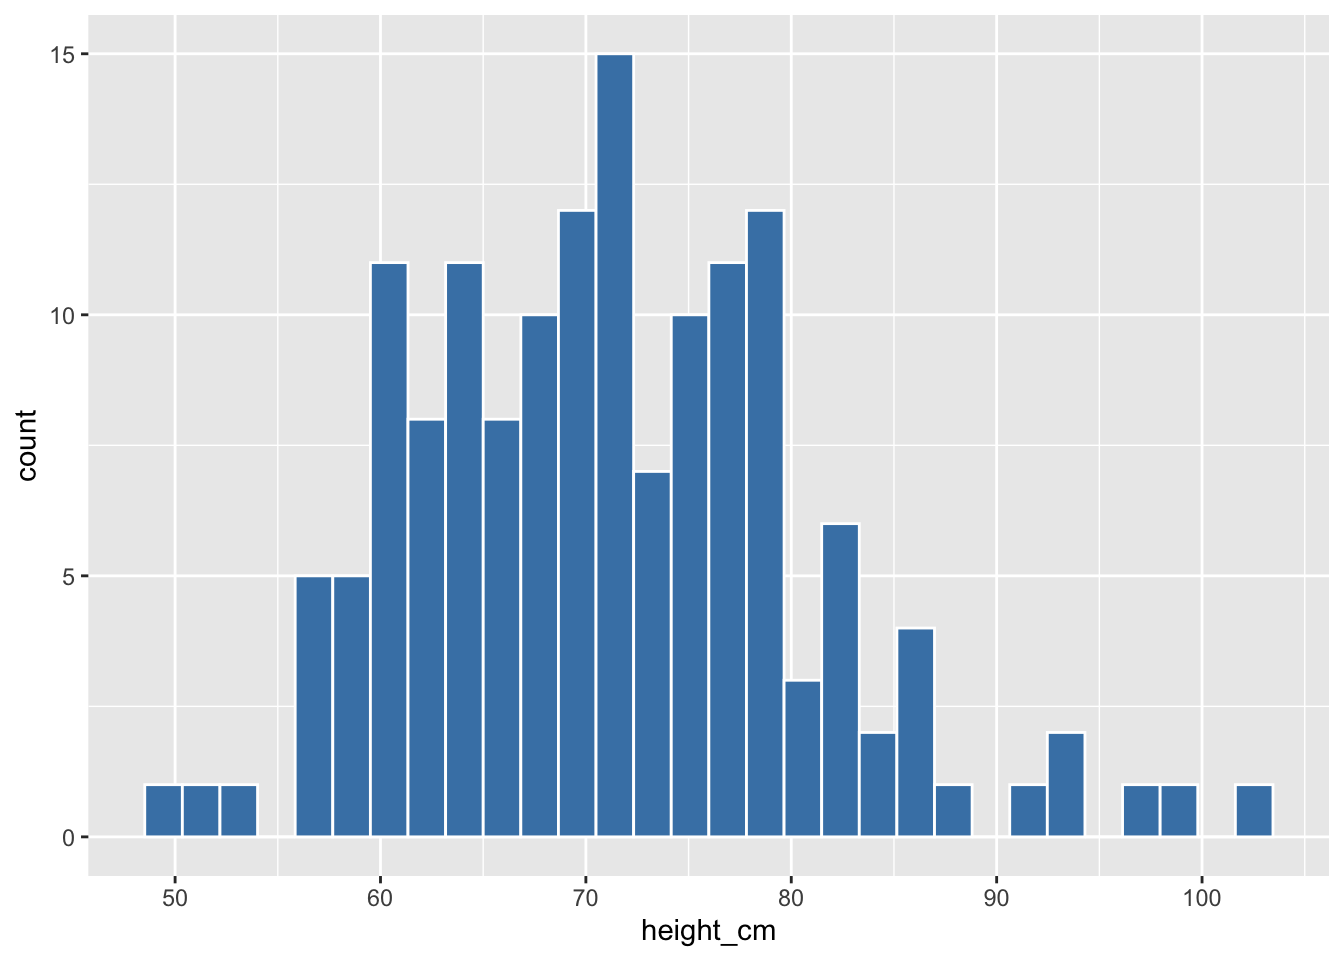
\includegraphics{data_on_display_ls02_scatter_files/figure-pdf/unnamed-chunk-15-1.pdf}

}

\end{figure}

In addition to changing the default color, now we will modify the
\texttt{size} aesthetic of the points by assigning it to a fixed number
(in millimeters). The default size is 1 mm, so let's chose a larger
value:

\begin{Shaded}
\begin{Highlighting}[]
\DocumentationTok{\#\#  Set size to 2 mm by ading \textasciigrave{}size = 2\textasciigrave{}}
\FunctionTok{ggplot}\NormalTok{(}\AttributeTok{data =}\NormalTok{ malidd, }
       \AttributeTok{mapping =} \FunctionTok{aes}\NormalTok{(}\AttributeTok{x =}\NormalTok{ age\_months, }
                     \AttributeTok{y =}\NormalTok{ viral\_load)) }\SpecialCharTok{+} 
  \FunctionTok{geom\_point}\NormalTok{(}\AttributeTok{color =} \StringTok{"steelblue"}\NormalTok{,       }\CommentTok{\# set color}
             \AttributeTok{size =} \DecValTok{2}\NormalTok{)                  }\CommentTok{\# set size (mm)}
\end{Highlighting}
\end{Shaded}

\begin{figure}[H]

{\centering 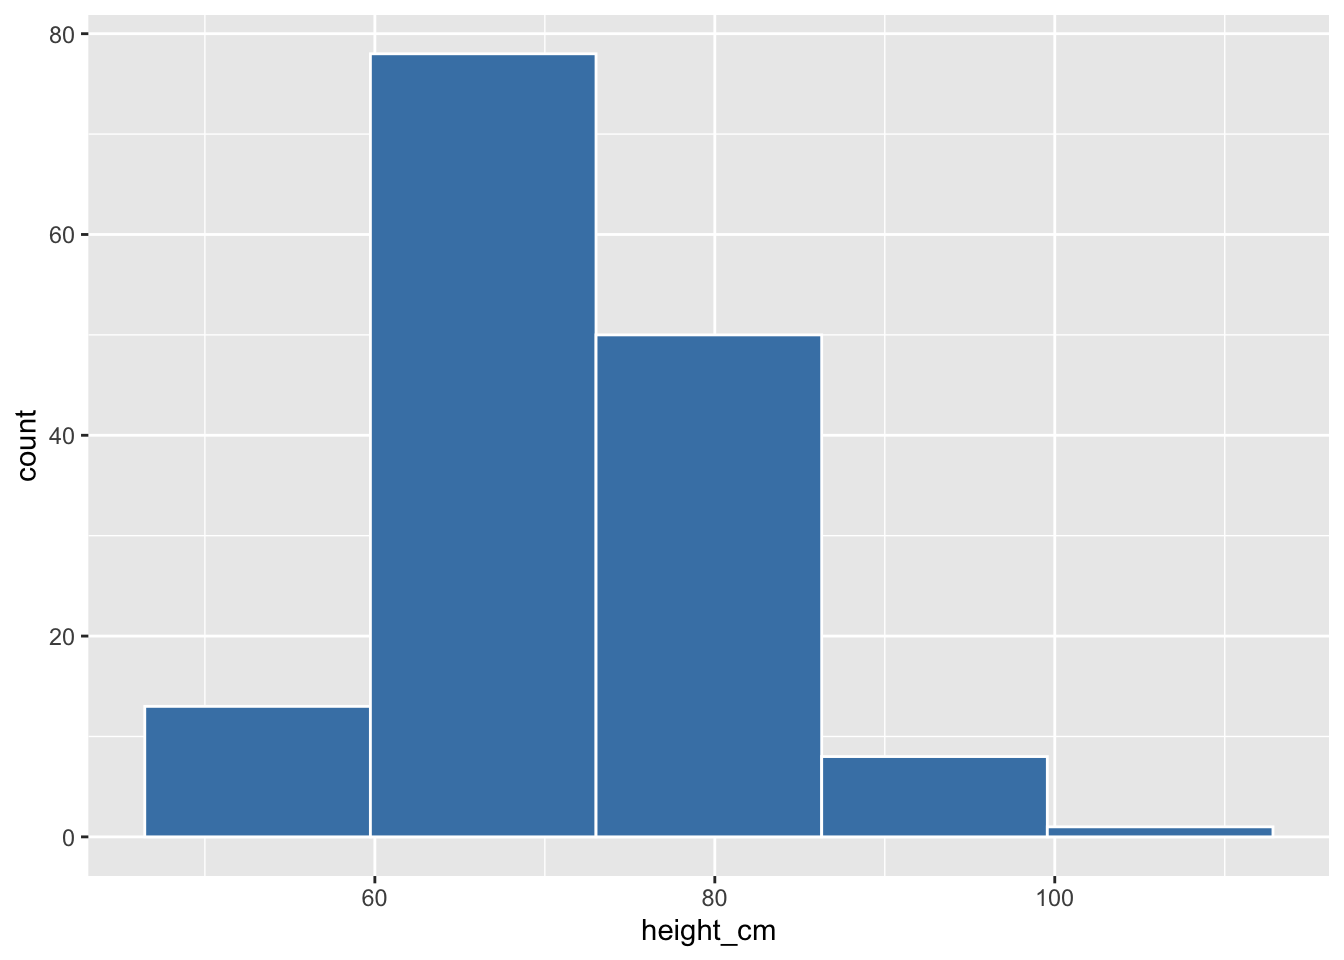
\includegraphics{data_on_display_ls02_scatter_files/figure-pdf/unnamed-chunk-16-1.pdf}

}

\end{figure}

The \texttt{alpha} aesthetic controls the level of opacity of
\texttt{geom}s. \texttt{alpha} is also numerical, and ranges from 0
(completely transparent) to the default of 1 (completely opaque). Let's
make our points more transparent by reducing the opacity:

\begin{Shaded}
\begin{Highlighting}[]
\DocumentationTok{\#\#  Set opacity to 75\% by adding \textasciigrave{}alpha = 0.75\textasciigrave{}}
\FunctionTok{ggplot}\NormalTok{(}\AttributeTok{data =}\NormalTok{ malidd, }
       \AttributeTok{mapping =} \FunctionTok{aes}\NormalTok{(}\AttributeTok{x =}\NormalTok{ age\_months, }
                     \AttributeTok{y =}\NormalTok{ viral\_load)) }\SpecialCharTok{+} 
  \FunctionTok{geom\_point}\NormalTok{(}\AttributeTok{color =} \StringTok{"steelblue"}\NormalTok{,       }\CommentTok{\# set color}
             \AttributeTok{size =} \DecValTok{2}\NormalTok{,                  }\CommentTok{\# set size (mm)}
             \AttributeTok{alpha =} \FloatTok{0.75}\NormalTok{)              }\CommentTok{\# set level of opacity}
\end{Highlighting}
\end{Shaded}

\begin{figure}[H]

{\centering 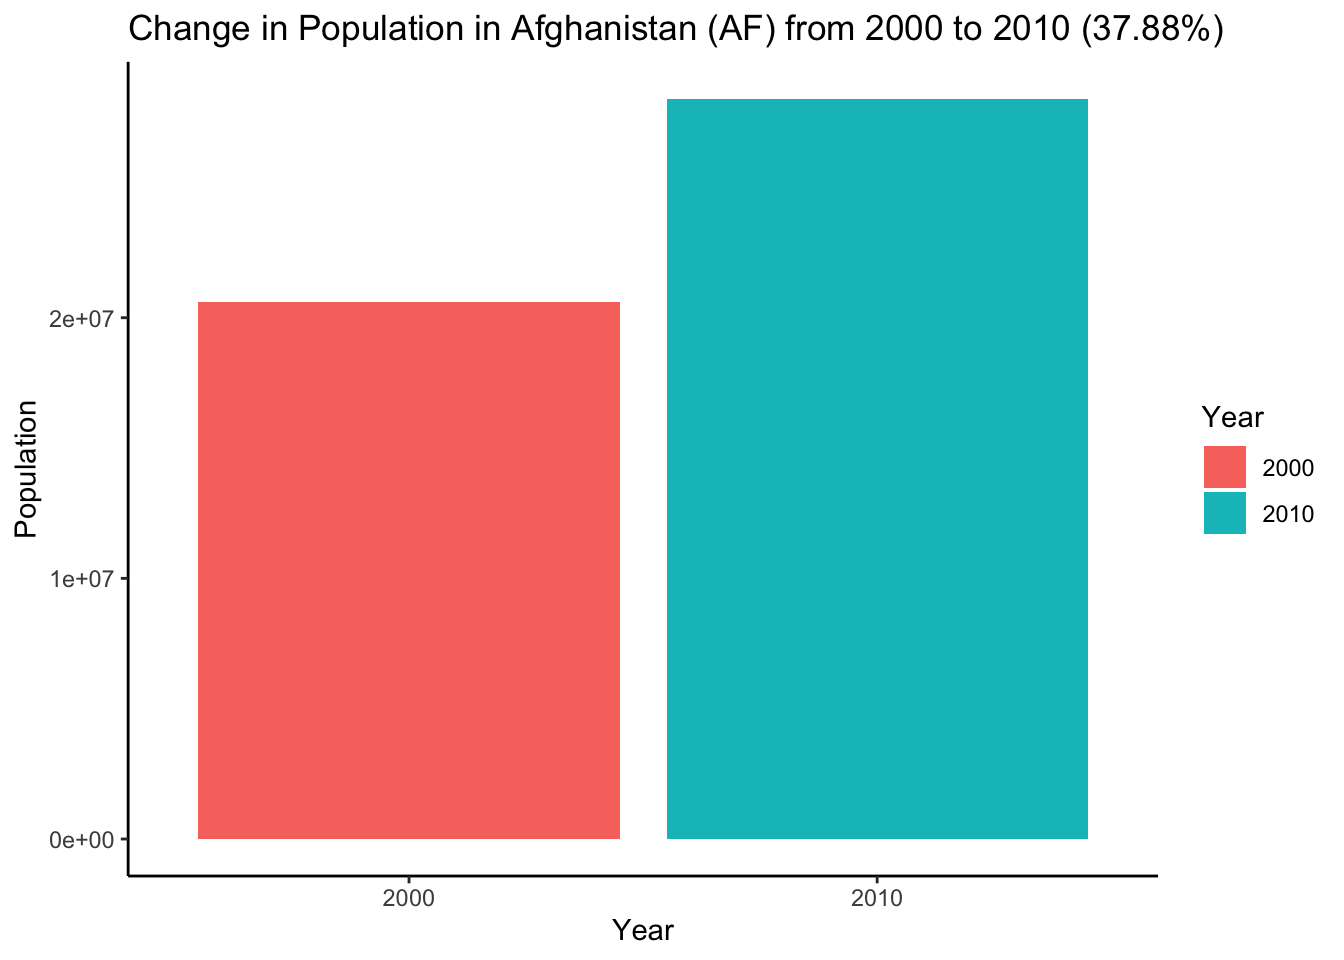
\includegraphics{data_on_display_ls02_scatter_files/figure-pdf/unnamed-chunk-17-1.pdf}

}

\end{figure}

Now we can see where multiple points overlap. This is a useful parameter
for scatter plots where there is \textbf{overplotting}.

Remember, changing the color, size, or opacity of our points here is not
conveying any information in the data - they are design choices we make
to create prettier plots.

\begin{tcolorbox}[enhanced jigsaw, colframe=quarto-callout-tip-color-frame, colbacktitle=quarto-callout-tip-color!10!white, titlerule=0mm, opacitybacktitle=0.6, breakable, toprule=.15mm, arc=.35mm, rightrule=.15mm, colback=white, bottomrule=.15mm, opacityback=0, toptitle=1mm, left=2mm, bottomtitle=1mm, title=\textcolor{quarto-callout-tip-color}{\faLightbulb}\hspace{0.5em}{Practice}, leftrule=.75mm, coltitle=black]

\begin{itemize}
\tightlist
\item
  Create a scatter plot with the same variables as the previous example,
  but change the color of the points to \texttt{cornflowerblue},
  increase the size of points to 3 mm and set the opacity to 60\%.
\end{itemize}

\end{tcolorbox}

\hypertarget{changing-shape-and-fill}{%
\subsubsection{\texorpdfstring{Changing \texttt{shape} and
\texttt{fill}}{Changing shape and fill}}\label{changing-shape-and-fill}}

We can change the appearance of points in a scatter plot with the
\texttt{shape} aesthetic.

To change the shape of your \texttt{geom}s to a fixed value, set
\texttt{shape} equal to a number corresponding to your desired shape.

\{ggplot2\} will accept the following numbers:

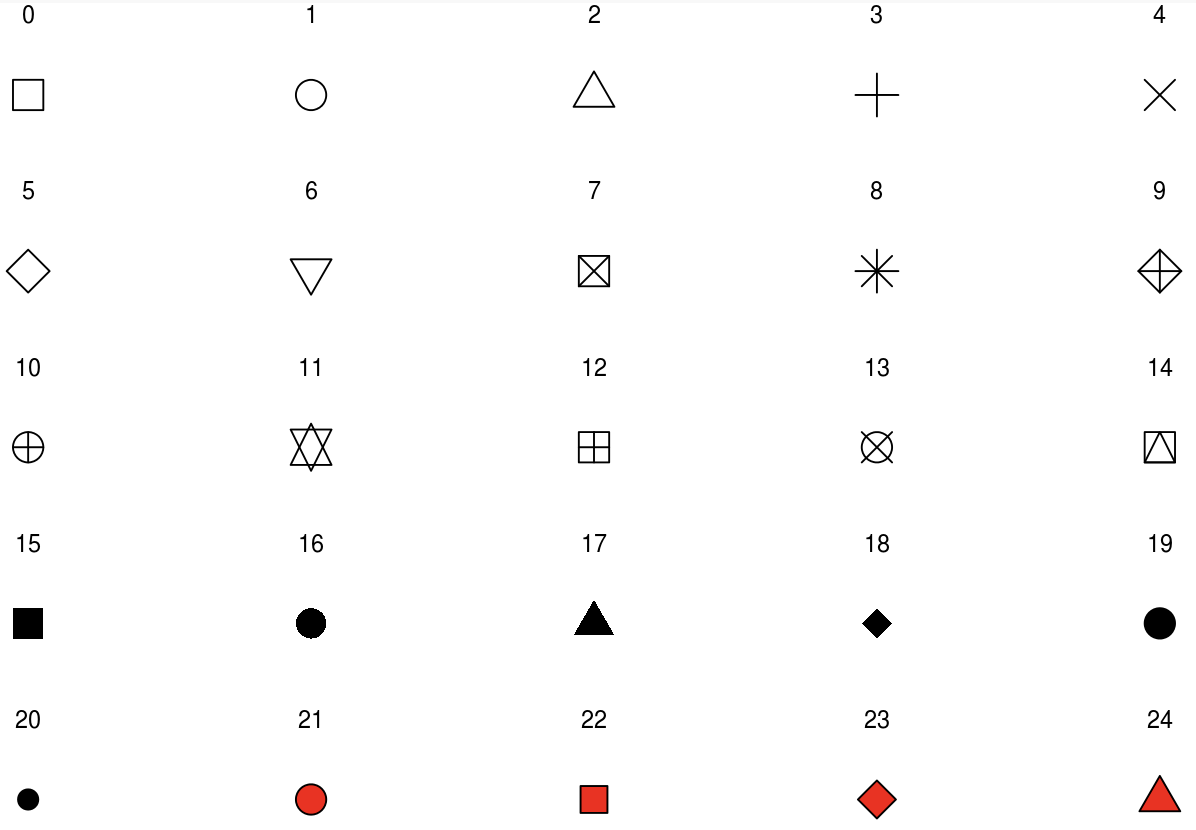
\includegraphics[width=4.16667in,height=\textheight]{images/ggplot_shapes.png}
Notice that some of the shapes are filled in with red. This indicates
that objects 21-24 are sensitive to both \texttt{color} and
\texttt{fill}, but the others are only sensitive to color.

First let's modify our original scatterplot by changing the shapes to a
something that can be filled in:

\begin{Shaded}
\begin{Highlighting}[]
\DocumentationTok{\#\# Set shape to fillable circles by adding \textasciigrave{}shape = 21\textasciigrave{}}

\FunctionTok{ggplot}\NormalTok{(}\AttributeTok{data =}\NormalTok{ malidd, }
       \AttributeTok{mapping =} \FunctionTok{aes}\NormalTok{(}\AttributeTok{x =}\NormalTok{ age\_months, }
                     \AttributeTok{y =}\NormalTok{ viral\_load)) }\SpecialCharTok{+} 
  \FunctionTok{geom\_point}\NormalTok{(}\AttributeTok{shape =} \DecValTok{21}\NormalTok{)                }\CommentTok{\# set shapes to display}
\end{Highlighting}
\end{Shaded}

\begin{figure}[H]

{\centering \includegraphics{data_on_display_ls02_scatter_files/figure-pdf/unnamed-chunk-20-1.pdf}

}

\end{figure}

Fillable shapes can have different colors for the outline and interior.
Changing the \texttt{color} aesthetic will only change the outline of
our points:

\begin{Shaded}
\begin{Highlighting}[]
\DocumentationTok{\#\# Set outline color of the shapes by adding \textasciigrave{}color = cyan4\textasciigrave{}}

\FunctionTok{ggplot}\NormalTok{(}\AttributeTok{data =}\NormalTok{ malidd, }
       \AttributeTok{mapping =} \FunctionTok{aes}\NormalTok{(}\AttributeTok{x =}\NormalTok{ age\_months, }
                     \AttributeTok{y =}\NormalTok{ viral\_load)) }\SpecialCharTok{+} 
  \FunctionTok{geom\_point}\NormalTok{(}\AttributeTok{shape =} \DecValTok{21}\NormalTok{,                }\CommentTok{\# set shapes to display}
             \AttributeTok{color =} \StringTok{"cyan4"}\NormalTok{)           }\CommentTok{\# set outline color}
\end{Highlighting}
\end{Shaded}

\begin{figure}[H]

{\centering \includegraphics{data_on_display_ls02_scatter_files/figure-pdf/unnamed-chunk-21-1.pdf}

}

\end{figure}

Now let's fill in the points:

\begin{Shaded}
\begin{Highlighting}[]
\DocumentationTok{\#\# Set interior color of the shapes by adding \textasciigrave{}fill = "seagreen"\textasciigrave{} }

\FunctionTok{ggplot}\NormalTok{(}\AttributeTok{data =}\NormalTok{ malidd, }
       \AttributeTok{mapping =} \FunctionTok{aes}\NormalTok{(}\AttributeTok{x =}\NormalTok{ age\_months, }
                     \AttributeTok{y =}\NormalTok{ viral\_load)) }\SpecialCharTok{+} 
  \FunctionTok{geom\_point}\NormalTok{(}\AttributeTok{shape =} \DecValTok{21}\NormalTok{,                }\CommentTok{\# set shapes to display}
             \AttributeTok{color =} \StringTok{"cyan4"}\NormalTok{,           }\CommentTok{\# set outline color}
             \AttributeTok{fill =} \StringTok{"seagreen"}\NormalTok{)         }\CommentTok{\# set fill color}
\end{Highlighting}
\end{Shaded}

\begin{figure}[H]

{\centering 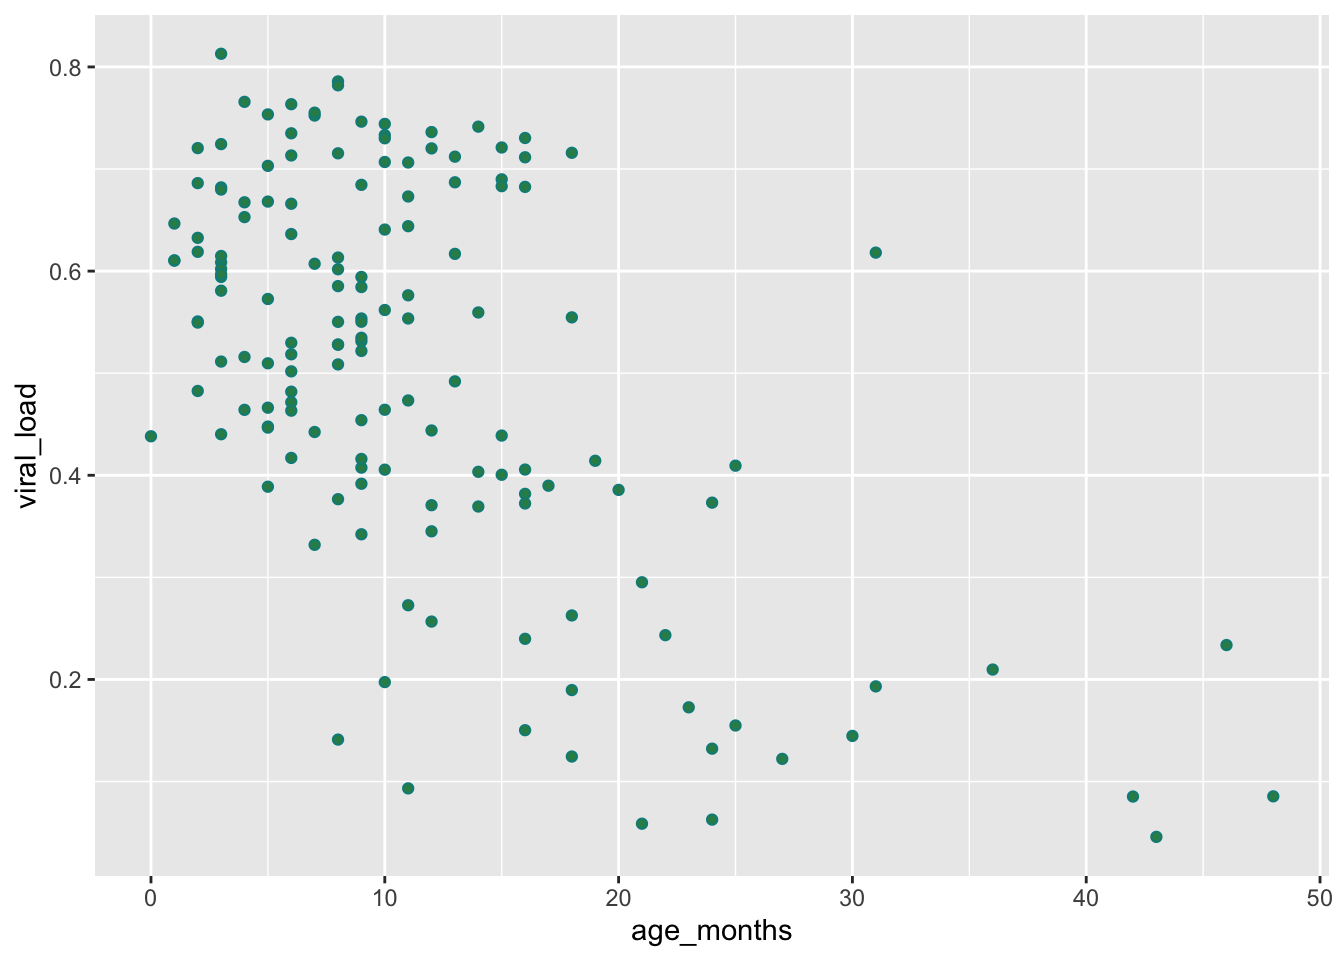
\includegraphics{data_on_display_ls02_scatter_files/figure-pdf/unnamed-chunk-22-1.pdf}

}

\end{figure}

We can improve the readability by increasing size and reducing opcaity
with \texttt{size} and \texttt{alpha}, like we did before:

\begin{Shaded}
\begin{Highlighting}[]
\FunctionTok{ggplot}\NormalTok{(}\AttributeTok{data =}\NormalTok{ malidd, }
       \AttributeTok{mapping =} \FunctionTok{aes}\NormalTok{(}\AttributeTok{x =}\NormalTok{ age\_months, }
                     \AttributeTok{y =}\NormalTok{ viral\_load)) }\SpecialCharTok{+} 
  \FunctionTok{geom\_point}\NormalTok{(}\AttributeTok{shape =} \DecValTok{21}\NormalTok{,                }\CommentTok{\# set shapes to display}
             \AttributeTok{color =} \StringTok{"cyan4"}\NormalTok{,           }\CommentTok{\# set outline color}
             \AttributeTok{fill =} \StringTok{"seagreen"}\NormalTok{,         }\CommentTok{\# set fill color}
             \AttributeTok{size =} \DecValTok{2}\NormalTok{,                  }\CommentTok{\# set size (mm)}
             \AttributeTok{alpha =} \FloatTok{0.75}\NormalTok{)              }\CommentTok{\# set level of opacity}
\end{Highlighting}
\end{Shaded}

\begin{figure}[H]

{\centering 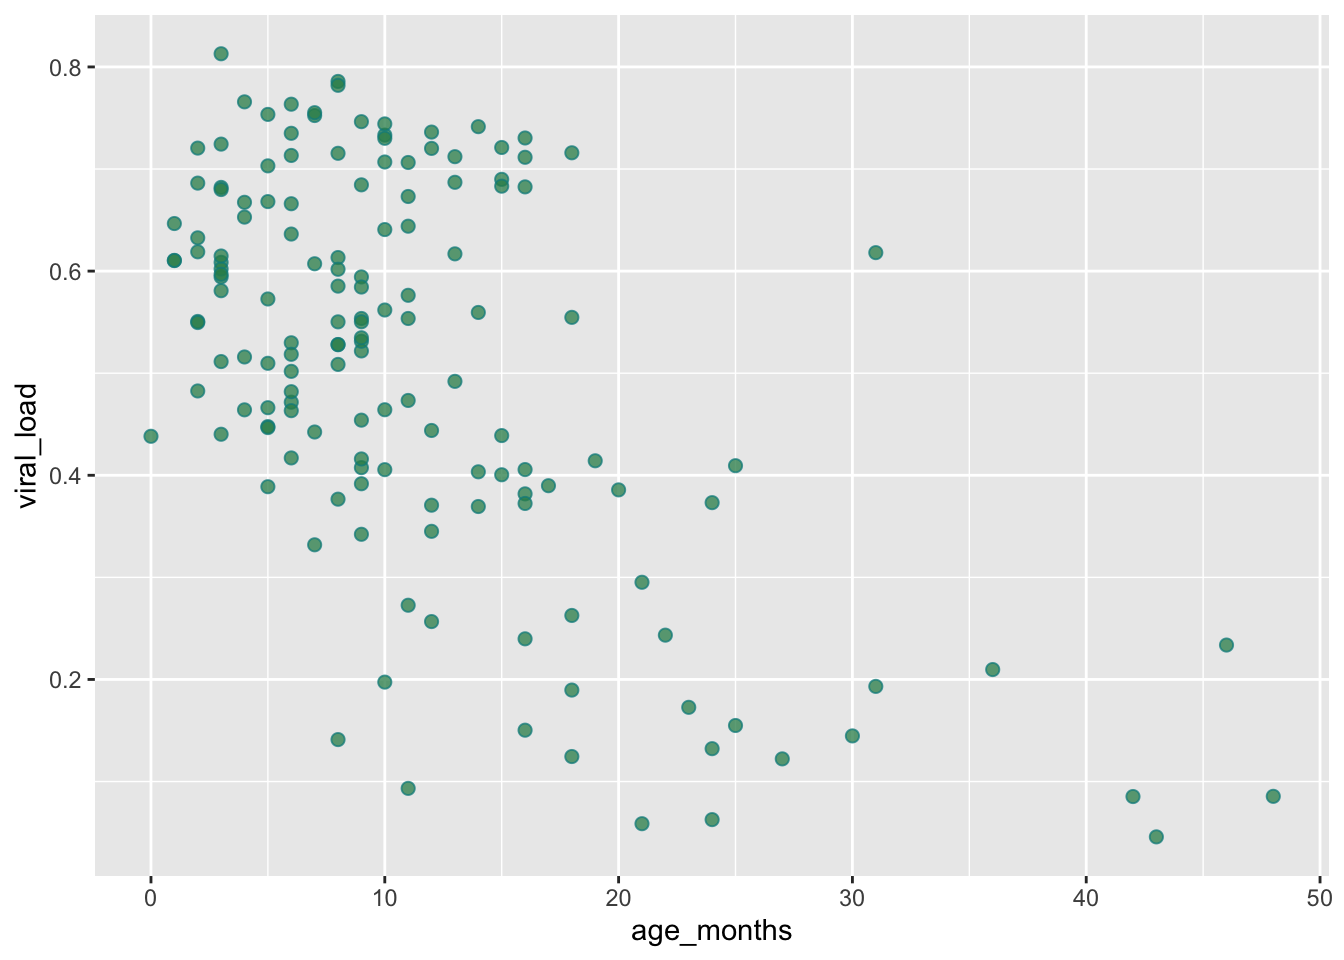
\includegraphics{data_on_display_ls02_scatter_files/figure-pdf/unnamed-chunk-23-1.pdf}

}

\end{figure}

\hypertarget{adding-a-trend-line}{%
\section{Adding a trend line}\label{adding-a-trend-line}}

It can be hard to view relationships or trends with just points alone.
Often we want to add a smoothing line in order to see what the trends
look like. This can be especially helpful when trying to understand
regressions.

To get a better idea of the relationship between these to variables, we
can add a trend line (also known as a best fit line or a smoothing
line).

To do this, we add the function \texttt{geom\_smooth()} to our scatter
plot:

\begin{Shaded}
\begin{Highlighting}[]
\FunctionTok{ggplot}\NormalTok{(}\AttributeTok{data =}\NormalTok{ malidd, }
       \AttributeTok{mapping =} \FunctionTok{aes}\NormalTok{(}\AttributeTok{x =}\NormalTok{ age\_months, }
                     \AttributeTok{y =}\NormalTok{ viral\_load)) }\SpecialCharTok{+} 
  \FunctionTok{geom\_point}\NormalTok{() }\SpecialCharTok{+}
  \FunctionTok{geom\_smooth}\NormalTok{()}
\end{Highlighting}
\end{Shaded}

\begin{verbatim}
`geom_smooth()` using method = 'loess' and formula = 'y ~ x'
\end{verbatim}

\begin{figure}[H]

{\centering 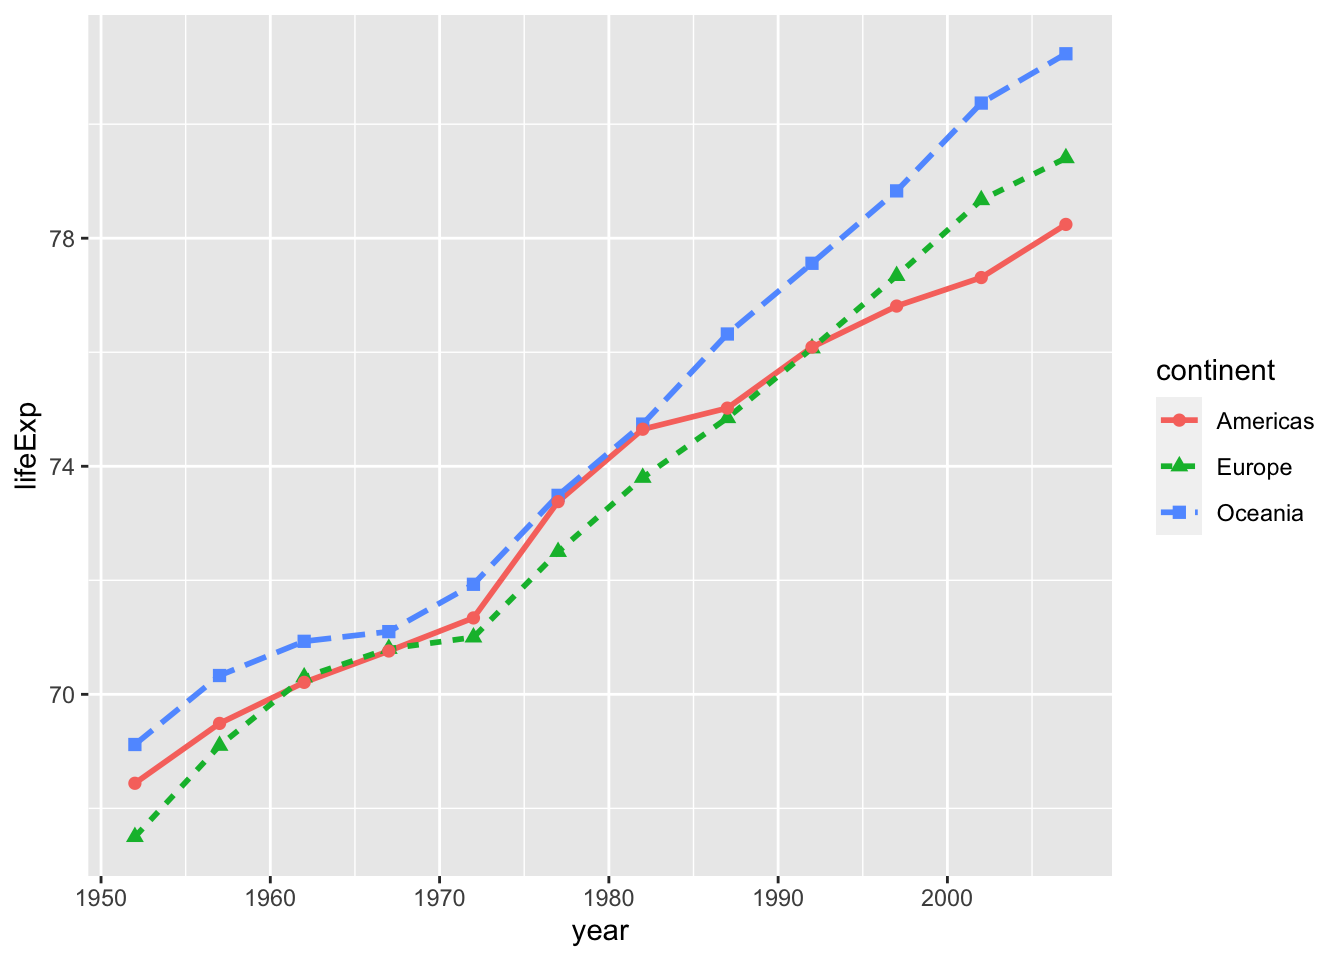
\includegraphics{data_on_display_ls02_scatter_files/figure-pdf/unnamed-chunk-24-1.pdf}

}

\end{figure}

The smoothing line comes after our points an another geometric layer
added onto our plot.

The default smoothing function used in this scatter plot is ``loess''
which stands for for \textbf{l}ocally \textbf{w}eighted \textbf{scatter
plot} \textbf{s}moothing. Loess smoothing is a process used by many
statistical softwares. In \{ggplot2\} this generally should be done when
you have less than 1000 points, otherwise it can be time consuming.

Many other smoothing functions can also be used in
\texttt{geom\_smooth()}.

Let's request a linear regression method. This time we will use a
generalized linear model by setting the \texttt{method} argument inside
\texttt{geom\_smooth()}:

\begin{Shaded}
\begin{Highlighting}[]
\DocumentationTok{\#\# Change to a linear smoothing function with \textasciigrave{}method = "glm"\textasciigrave{}}
\FunctionTok{ggplot}\NormalTok{(}\AttributeTok{data =}\NormalTok{ malidd, }
       \AttributeTok{mapping =} \FunctionTok{aes}\NormalTok{(}\AttributeTok{x =}\NormalTok{ age\_months, }
                     \AttributeTok{y =}\NormalTok{ viral\_load)) }\SpecialCharTok{+} 
  \FunctionTok{geom\_point}\NormalTok{() }\SpecialCharTok{+}
  \FunctionTok{geom\_smooth}\NormalTok{(}\AttributeTok{method =} \StringTok{"glm"}\NormalTok{)}
\end{Highlighting}
\end{Shaded}

\begin{verbatim}
`geom_smooth()` using formula = 'y ~ x'
\end{verbatim}

\begin{figure}[H]

{\centering \includegraphics{data_on_display_ls02_scatter_files/figure-pdf/unnamed-chunk-25-1.pdf}

}

\end{figure}

By default, 95\% confidence limits for these lines are displayed.

You can suppress the confidence bands by including the argument
\texttt{se\ =\ FALSE} inside \texttt{geom\_smooth()}:

\begin{Shaded}
\begin{Highlighting}[]
\DocumentationTok{\#\# Remove confidence interval bands by adding \textasciigrave{}se = FALSE\textasciigrave{}}
\FunctionTok{ggplot}\NormalTok{(}\AttributeTok{data =}\NormalTok{ malidd, }
       \AttributeTok{mapping =} \FunctionTok{aes}\NormalTok{(}\AttributeTok{x =}\NormalTok{ age\_months, }
                     \AttributeTok{y =}\NormalTok{ viral\_load)) }\SpecialCharTok{+} 
  \FunctionTok{geom\_point}\NormalTok{() }\SpecialCharTok{+}
  \FunctionTok{geom\_smooth}\NormalTok{(}\AttributeTok{method =} \StringTok{"glm"}\NormalTok{,}
              \AttributeTok{se =} \ConstantTok{FALSE}\NormalTok{)}
\end{Highlighting}
\end{Shaded}

\begin{verbatim}
`geom_smooth()` using formula = 'y ~ x'
\end{verbatim}

\begin{figure}[H]

{\centering \includegraphics{data_on_display_ls02_scatter_files/figure-pdf/unnamed-chunk-26-1.pdf}

}

\end{figure}

In addition to changing the method, let's add the \texttt{color}
argument inside \texttt{geom\_smooth()} to change the color of the line.

\begin{Shaded}
\begin{Highlighting}[]
\DocumentationTok{\#\# Change the color of the trend line by adding \textasciigrave{}color = "darkred"\textasciigrave{}}
\FunctionTok{ggplot}\NormalTok{(}\AttributeTok{data =}\NormalTok{ malidd, }
       \AttributeTok{mapping =} \FunctionTok{aes}\NormalTok{(}\AttributeTok{x =}\NormalTok{ age\_months, }
                     \AttributeTok{y =}\NormalTok{ viral\_load)) }\SpecialCharTok{+} 
  \FunctionTok{geom\_point}\NormalTok{() }\SpecialCharTok{+}
  \FunctionTok{geom\_smooth}\NormalTok{(}\AttributeTok{method =} \StringTok{"glm"}\NormalTok{,}
              \AttributeTok{se =} \ConstantTok{FALSE}\NormalTok{,}
              \AttributeTok{color =} \StringTok{"darkred"}\NormalTok{)}
\end{Highlighting}
\end{Shaded}

\begin{verbatim}
`geom_smooth()` using formula = 'y ~ x'
\end{verbatim}

\begin{figure}[H]

{\centering \includegraphics{data_on_display_ls02_scatter_files/figure-pdf/unnamed-chunk-27-1.pdf}

}

\end{figure}

This linear regression concurs with what we initially observed in the
first scatter plot. A \emph{negative relationship} exists between
\texttt{age\_months} and \texttt{viral\_load}: as age increases, viral
load tends to decrease.

Let's add a third variable from the \texttt{malidd} dataset
called\texttt{vomit}. This which is a binary variable that records
whether or not the patient vomited. We will add the \texttt{vomit}
variable to the plot by mapping it to the color aesthetic. We will again
change the smoothing method to generalized additive model
(``\texttt{gam}'') and make some aesthetic modifications to the line in
the \texttt{geom\_smooth()} layer.

\begin{Shaded}
\begin{Highlighting}[]
\FunctionTok{ggplot}\NormalTok{(}\AttributeTok{data =}\NormalTok{ malidd, }
       \AttributeTok{mapping =} \FunctionTok{aes}\NormalTok{(}\AttributeTok{x =}\NormalTok{ age\_months, }
                     \AttributeTok{y =}\NormalTok{ viral\_load)) }\SpecialCharTok{+} 
  \FunctionTok{geom\_point}\NormalTok{(}\AttributeTok{mapping =} \FunctionTok{aes}\NormalTok{(}\AttributeTok{color =} \FunctionTok{factor}\NormalTok{(vomit))) }\SpecialCharTok{+}
  \FunctionTok{geom\_smooth}\NormalTok{(}\AttributeTok{method =} \StringTok{"gam"}\NormalTok{, }
              \AttributeTok{size =} \FloatTok{1.5}\NormalTok{,}
              \AttributeTok{color =} \StringTok{"darkgray"}\NormalTok{)}
\end{Highlighting}
\end{Shaded}

\begin{verbatim}
Warning: Using `size` aesthetic for lines was deprecated in ggplot2 3.4.0.
i Please use `linewidth` instead.
\end{verbatim}

\begin{verbatim}
`geom_smooth()` using formula = 'y ~ s(x, bs = "cs")'
\end{verbatim}

\begin{figure}[H]

{\centering \includegraphics{data_on_display_ls02_scatter_files/figure-pdf/unnamed-chunk-28-1.pdf}

}

\end{figure}

Observe the distribution of blue points (children who vomited) compared
to red points (children who did not vomit). The blue points mostly occur
above the trend line. This shows that higher viral loads were not only
associated with younger children, but that children with higher viral
loads were more likely to exhibit symptoms of vomiting.

\begin{tcolorbox}[enhanced jigsaw, colframe=quarto-callout-tip-color-frame, colbacktitle=quarto-callout-tip-color!10!white, titlerule=0mm, opacitybacktitle=0.6, breakable, toprule=.15mm, arc=.35mm, rightrule=.15mm, colback=white, bottomrule=.15mm, opacityback=0, toptitle=1mm, left=2mm, bottomtitle=1mm, title=\textcolor{quarto-callout-tip-color}{\faLightbulb}\hspace{0.5em}{Practice}, leftrule=.75mm, coltitle=black]

\begin{itemize}
\item
  Create a scatter plot with the \texttt{age\_months} and
  \texttt{height\_cm} variables. Set the color of the points to
  ``steelblue'', the size to 2.5mm, the opacity to 80\%. Then add trend
  line with the smoothing method ``lm'' (linear model). To make the
  trend line stand out, set its color to ``indianred3''.
\item
  Recreate the plot you made in the previous question, but this time
  adapt the code to change the shape of the points to tilted rectangles
  (number 23), and add the body temperature variable (\texttt{temp}) by
  \textbf{mapping} it to fill color of the points.
\end{itemize}

\begin{Shaded}
\begin{Highlighting}[]
\DocumentationTok{\#\# Type and view your answer:}
\NormalTok{age\_height\_3 }\OtherTok{\textless{}{-}}  \StringTok{"YOUR ANSWER HERE"}
\NormalTok{age\_height\_3}
\end{Highlighting}
\end{Shaded}

\end{tcolorbox}

\hypertarget{summary}{%
\section{Summary}\label{summary}}

Scatter plots display the relationship between two numerical variables.

With medium to large datasets, you may need to play around with the
different modifications to scatter plots we saw such as adding trend
lines, changing the color, size, shape, fill, or opacity of the points.
This tweaking is often a fun part of data visualization, since you'll
have the chance to see different relationships emerge as you tinker with
your plots.

The following team members contributed to this lesson:

\hypertarget{references-1}{%
\section*{References}\label{references-1}}

\markright{References}

Some material in this lesson was adapted from the following sources:

\begin{itemize}
\tightlist
\item
  Ismay, Chester, and Albert Y. Kim. 2022. \emph{A ModernDive into R and
  the Tidyverse}. \url{https://moderndive.com/}.
\item
  Kabacoff, Rob. 2020. \emph{Data Visualization with R}.
  \url{https://rkabacoff.github.io/datavis/}.
\item
  Giroux-Bougard, Xavier, Maxwell Farrell, Amanda Winegardner, Étienne
  Low-Decarie and Monica Granados. 2020. \emph{Workshop 3: Introduction
  to Data Visualisation with \{ggplot2\}}.
  \url{http://r.qcbs.ca/workshop03/book-en/}.
\end{itemize}

\hypertarget{solutions-1}{%
\section{Solutions}\label{solutions-1}}

\begin{Shaded}
\begin{Highlighting}[]
\FunctionTok{.SOLUTION\_age\_height}\NormalTok{()}
\end{Highlighting}
\end{Shaded}

\begin{verbatim}
ggplot(data = malidd,
             mapping = aes(x = age_months, 
                           y = height_cm)) +
      geom_point()
\end{verbatim}

\begin{Shaded}
\begin{Highlighting}[]
\FunctionTok{.SOLUTION\_age\_height\_respi}\NormalTok{()}
\end{Highlighting}
\end{Shaded}

\begin{verbatim}
ggplot(data = malidd, 
             mapping = aes(x = age_months, 
                           y = viral_load)) + 
      geom_point(mapping = aes(color = freqrespi))
\end{verbatim}

\begin{Shaded}
\begin{Highlighting}[]
\FunctionTok{.SOLUTION\_age\_viral\_respi}\NormalTok{() }
\end{Highlighting}
\end{Shaded}

\begin{verbatim}
ggplot(data = malidd, 
             mapping = aes(x = age_months, 
                           y = viral_load)) + 
      geom_point(mapping = aes(color = freqrespi))
\end{verbatim}

\begin{Shaded}
\begin{Highlighting}[]
\FunctionTok{.SOLUTION\_age\_height\_fever}\NormalTok{()}
\end{Highlighting}
\end{Shaded}

\begin{verbatim}
ggplot(data = malidd, 
             mapping = aes(x = age_months, 
                           y = height_cm)) + 
      geom_point(mapping = aes(color = factor(fever)))
\end{verbatim}

\begin{Shaded}
\begin{Highlighting}[]
\FunctionTok{.SOLUTION\_age\_viral\_blue}\NormalTok{()}
\end{Highlighting}
\end{Shaded}

\begin{verbatim}
ggplot(data = malidd, 
             mapping = aes(x = age_months, 
                           y = viral_load)) + 
      geom_point(color = "cornflowerblue",
                 size = 3,
                 alpha = 0.6)
\end{verbatim}

\begin{Shaded}
\begin{Highlighting}[]
\FunctionTok{.SOLUTION\_age\_height\_2}\NormalTok{()}
\end{Highlighting}
\end{Shaded}

\begin{verbatim}
ggplot(data = malidd, 
          mapping = aes(x = age_months, 
                        y = height_cm)) + 
      geom_point(color = "steelblue",
                 size = 2.5,
                 alpha = 0.8) +
      geom_smooth(method = "lm", color = "indianred3")
\end{verbatim}

\begin{Shaded}
\begin{Highlighting}[]
\FunctionTok{.SOLUTION\_age\_height\_3}\NormalTok{()}
\end{Highlighting}
\end{Shaded}

\begin{verbatim}
ggplot(data = malidd, 
          mapping = aes(x = age_months, y = height_cm)) + 
      geom_point(color = "steelblue",
                 size = 2.5,
                 alpha = 0.8,
                 shape = 23,
                 mapping = aes(fill = temp)) +
      geom_smooth(method = "lm", color = "indianred3")
\end{verbatim}

\bookmarksetup{startatroot}

\hypertarget{lines-scales-and-labels}{%
\chapter{Lines, scales, and labels}\label{lines-scales-and-labels}}

\hypertarget{learning-objectives-2}{%
\section{Learning Objectives}\label{learning-objectives-2}}

\begin{enumerate}
\def\labelenumi{\arabic{enumi}.}
\tightlist
\item
  You can create \textbf{line graphs} to visualize relationships between
  two numerical variables with \textbf{\texttt{geom\_line()}}.
\item
  You can \textbf{add points} to a line graph with
  \texttt{geom\_point()}.
\item
  You can use aesthetics like \texttt{color}, \textbf{\texttt{size}},
  \textbf{\texttt{color}}, and \textbf{\texttt{linetype}} to modify line
  graphs.
\item
  You can \textbf{manipulate axis scales} for continuous data with
  \textbf{\texttt{scale\_*\_continuous()}} and scale\_*\_log10().
\item
  You can \textbf{add labels} to a plot such as a
  \textbf{\texttt{title}}, \textbf{\texttt{subtitle}}, or
  \textbf{\texttt{caption}} with the \textbf{\texttt{labs()}} function.
\end{enumerate}

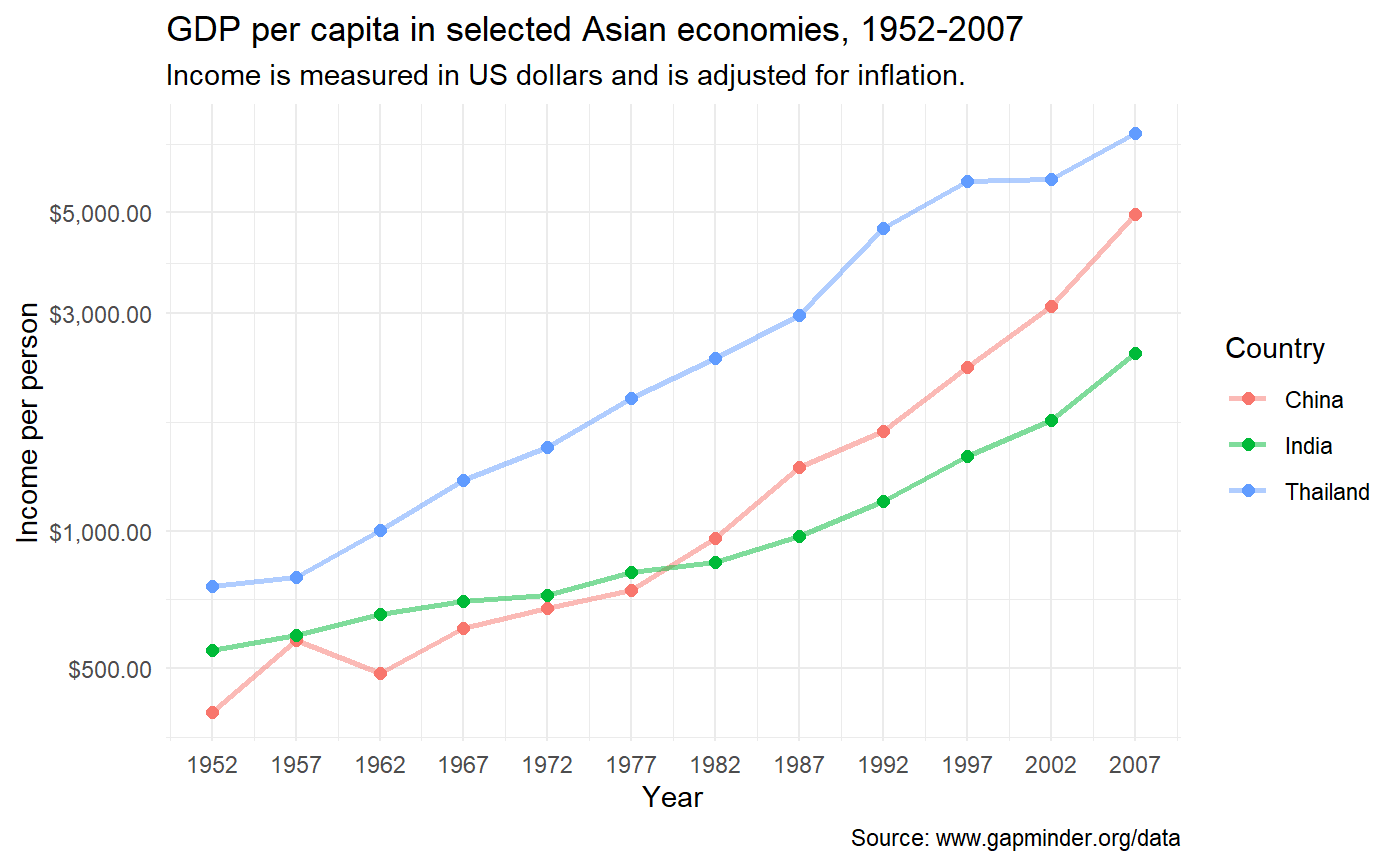
\includegraphics{images/paste-3755C0EB.png}

\hypertarget{introduction-2}{%
\section{Introduction}\label{introduction-2}}

Line graphs are used to show \textbf{relationships} between two
\textbf{numerical variables}, just like scatterplots. They are
especially useful when the variable on the x-axis, also called the
\emph{explanatory} variable, is of a \textbf{sequential} nature. In
other words, there is an inherent ordering to the variable.

The most common examples of line graphs have some notion of \textbf{time
on the x-axis}: hours, days, weeks, years, etc. Since time is
sequential, we connect consecutive observations of the variable on the
y-axis with a line. Line graphs that have some notion of time on the
x-axis are also called \textbf{time series plots}.

\hypertarget{packages-1}{%
\section{Packages}\label{packages-1}}

\begin{Shaded}
\begin{Highlighting}[]
\DocumentationTok{\#\# Load packages}
\NormalTok{pacman}\SpecialCharTok{::}\FunctionTok{p\_load}\NormalTok{(tidyverse, }
\NormalTok{               gapminder, }
\NormalTok{               here)}
\end{Highlighting}
\end{Shaded}

\hypertarget{the-gapminder-data-frame}{%
\section{\texorpdfstring{The \texttt{gapminder} data
frame}{The gapminder data frame}}\label{the-gapminder-data-frame}}

In February 2006, a Swedish physician and data advocate named Hans
Rosling gave a famous TED talk titled
\href{https://www.ted.com/talks/hans_rosling_shows_the_best_stats_you_ve_ever_seen}{``The
best stats you've ever seen''} where he presented global economic,
health, and development data complied by the Gapminder Foundation.

\begin{figure}

{\centering 

\href{https://www.gapminder.org/tools/}{\includegraphics{images/paste-6726AD73.png}}

}

\caption{Interactive data visualization tools with up-to-date data are
available on the Gapminder's website.}

\end{figure}

We can access a clean subset of this data with the R package
\{\textbf{gapminder}\}, which we just loaded.

\begin{Shaded}
\begin{Highlighting}[]
\DocumentationTok{\#\# Load gapminder data frame from the gapminder package}
\FunctionTok{data}\NormalTok{(gapminder, }\AttributeTok{package=}\StringTok{"gapminder"}\NormalTok{)}

\DocumentationTok{\#\# Print dataframe}
\NormalTok{gapminder}
\end{Highlighting}
\end{Shaded}

\begin{verbatim}
# A tibble: 10 x 6
   country     continent  year lifeExp      pop gdpPercap
   <fct>       <fct>     <int>   <dbl>    <int>     <dbl>
 1 Afghanistan Asia       1952    28.8  8425333      779.
 2 Afghanistan Asia       1957    30.3  9240934      821.
 3 Afghanistan Asia       1962    32.0 10267083      853.
 4 Afghanistan Asia       1967    34.0 11537966      836.
 5 Afghanistan Asia       1972    36.1 13079460      740.
 6 Afghanistan Asia       1977    38.4 14880372      786.
 7 Afghanistan Asia       1982    39.9 12881816      978.
 8 Afghanistan Asia       1987    40.8 13867957      852.
 9 Afghanistan Asia       1992    41.7 16317921      649.
10 Afghanistan Asia       1997    41.8 22227415      635.
\end{verbatim}

Each row in this table corresponds to a country-year combination. For
each row, we have 6 columns:

\begin{enumerate}
\def\labelenumi{\arabic{enumi})}
\item
  \textbf{\texttt{country}}: Country name
\item
  \textbf{\texttt{continent}}: Geographic region of the world
\item
  \textbf{\texttt{year}}: Calendar year
\item
  \textbf{\texttt{lifeExp}}: Average number of years a newborn child
  would live if current mortality patterns were to stay the same
\item
  \textbf{\texttt{pop}}: Total population
\item
  \textbf{\texttt{gdpPercap}}: Gross domestic product per person
  (inflation-adjusted US dollars)
\end{enumerate}

The \texttt{str()} function can tell us more about these variables.

\begin{Shaded}
\begin{Highlighting}[]
\DocumentationTok{\#\# Data structure}
\FunctionTok{str}\NormalTok{(gapminder)}
\end{Highlighting}
\end{Shaded}

\begin{verbatim}
tibble [1,704 x 6] (S3: tbl_df/tbl/data.frame)
 $ country  : Factor w/ 142 levels "Afghanistan",..: 1 1 1 1 1 1 1 1 1 1 ...
 $ continent: Factor w/ 5 levels "Africa","Americas",..: 3 3 3 3 3 3 3 3 3 3 ...
 $ year     : int [1:1704] 1952 1957 1962 1967 1972 1977 1982 1987 1992 1997 ...
 $ lifeExp  : num [1:1704] 28.8 30.3 32 34 36.1 ...
 $ pop      : int [1:1704] 8425333 9240934 10267083 11537966 13079460 14880372 12881816 13867957 16317921 22227415 ...
 $ gdpPercap: num [1:1704] 779 821 853 836 740 ...
\end{verbatim}

This version of the \textbf{\texttt{gapminder}} dataset contains
information for \textbf{142 countries}, divided in to \textbf{5
continents}.

\includegraphics{images/gap_map.png}

\begin{Shaded}
\begin{Highlighting}[]
\DocumentationTok{\#\# Data summary}
\FunctionTok{summary}\NormalTok{(gapminder)}
\end{Highlighting}
\end{Shaded}

\begin{verbatim}
        country        continent        year         lifeExp     
 Afghanistan:  12   Africa  :624   Min.   :1952   Min.   :23.60  
 Albania    :  12   Americas:300   1st Qu.:1966   1st Qu.:48.20  
 Algeria    :  12   Asia    :396   Median :1980   Median :60.71  
 Angola     :  12   Europe  :360   Mean   :1980   Mean   :59.47  
 Argentina  :  12   Oceania : 24   3rd Qu.:1993   3rd Qu.:70.85  
 Australia  :  12                  Max.   :2007   Max.   :82.60  
 (Other)    :1632                                                
      pop              gdpPercap       
 Min.   :6.001e+04   Min.   :   241.2  
 1st Qu.:2.794e+06   1st Qu.:  1202.1  
 Median :7.024e+06   Median :  3531.8  
 Mean   :2.960e+07   Mean   :  7215.3  
 3rd Qu.:1.959e+07   3rd Qu.:  9325.5  
 Max.   :1.319e+09   Max.   :113523.1  
                                       
\end{verbatim}

Data are recorded every 5 years from 1952 to 2007 (a total of 12 years).

Let's say we want to visualize the relationship between time
(\texttt{year}) and life expectancy (\texttt{lifeExp}).

For now let's just focus on one country - United States. First, we need
to create a new data frame with only the data from this country.

\begin{Shaded}
\begin{Highlighting}[]
\DocumentationTok{\#\# Select US cases}
\NormalTok{gap\_US }\OtherTok{\textless{}{-}}\NormalTok{ dplyr}\SpecialCharTok{::}\FunctionTok{filter}\NormalTok{(gapminder,}
\NormalTok{                        country }\SpecialCharTok{==} \StringTok{"United States"}\NormalTok{)}

\NormalTok{gap\_US}
\end{Highlighting}
\end{Shaded}

\begin{verbatim}
# A tibble: 10 x 6
   country       continent  year lifeExp       pop gdpPercap
   <fct>         <fct>     <int>   <dbl>     <int>     <dbl>
 1 United States Americas   1952    68.4 157553000    13990.
 2 United States Americas   1957    69.5 171984000    14847.
 3 United States Americas   1962    70.2 186538000    16173.
 4 United States Americas   1967    70.8 198712000    19530.
 5 United States Americas   1972    71.3 209896000    21806.
 6 United States Americas   1977    73.4 220239000    24073.
 7 United States Americas   1982    74.6 232187835    25010.
 8 United States Americas   1987    75.0 242803533    29884.
 9 United States Americas   1992    76.1 256894189    32004.
10 United States Americas   1997    76.8 272911760    35767.
\end{verbatim}

\begin{tcolorbox}[enhanced jigsaw, colframe=quarto-callout-note-color-frame, colbacktitle=quarto-callout-note-color!10!white, titlerule=0mm, opacitybacktitle=0.6, breakable, toprule=.15mm, arc=.35mm, rightrule=.15mm, colback=white, bottomrule=.15mm, opacityback=0, toptitle=1mm, left=2mm, bottomtitle=1mm, title=\textcolor{quarto-callout-note-color}{\faInfo}\hspace{0.5em}{Reminder}, leftrule=.75mm, coltitle=black]

The code above is a covered in our course on Data Wrangling using the
\{dplyr\} package. Data wrangling is the process of transforming and
modifying existing data with the intent of making it more appropriate
for analysis purposes. For example, this code segments used the
\texttt{filter()} function to create a new data frame (\texttt{gap\_US})
by choosing only a subset of rows of original \texttt{gapminder} data
frame (only those that have ``United States'' in the \texttt{country}
column).

\end{tcolorbox}

\hypertarget{line-graphs-via-geom_line}{%
\section{\texorpdfstring{Line graphs via
\texttt{geom\_line()}}{Line graphs via geom\_line()}}\label{line-graphs-via-geom_line}}

Now we're ready to feed the \texttt{gap\_US} data frame to
\texttt{ggplot()}, mapping \textbf{time} in years on the horizontal x
axis and \textbf{life expectancy} on the vertical y axis.

We can visualize this time series data by using \texttt{geom\_line()} to
create a line graph, instead of using \texttt{geom\_point()} like we
used previously to create scatterplots:

\begin{Shaded}
\begin{Highlighting}[]
\DocumentationTok{\#\# Simple line graph}
\FunctionTok{ggplot}\NormalTok{(}\AttributeTok{data =}\NormalTok{ gap\_US, }
       \AttributeTok{mapping =} \FunctionTok{aes}\NormalTok{(}\AttributeTok{x =}\NormalTok{ year, }
                     \AttributeTok{y =}\NormalTok{ lifeExp)) }\SpecialCharTok{+}
  \FunctionTok{geom\_line}\NormalTok{() }
\end{Highlighting}
\end{Shaded}

\begin{figure}[H]

{\centering \includegraphics{data_on_display_ls03_line_graphs_files/figure-pdf/unnamed-chunk-7-1.pdf}

}

\end{figure}

Much as with the \texttt{ggplot()} code that created the scatterplot of
age and viral load with \texttt{geom\_point()}, let's break down this
code piece-by-piece in terms of the grammar of graphics:

Within the \texttt{ggplot()} function call, we specify two of the
components of the grammar of graphics as arguments:

\begin{enumerate}
\def\labelenumi{\arabic{enumi}.}
\tightlist
\item
  The \texttt{data} to be the \texttt{gap\_US} data frame by setting
  \texttt{data\ =\ gap\_US}.
\item
  The \texttt{aes}thetic \texttt{mapping} by setting
  \texttt{mapping\ =\ aes(x\ =\ year,\ y\ =\ lifeExp)}. Specifically,
  the variable \texttt{year} maps to the \texttt{x} position aesthetic,
  while the variable \texttt{lifeExp} maps to the \texttt{y} position
  aesthetic.
\end{enumerate}

After telling R which data and aesthetic mappings we wanted to plot we
then added the third essential component, the \texttt{geom}etric object
using the \texttt{+} sign, In this case, the geometric object was set to
lines using \texttt{geom\_line()}.

\begin{tcolorbox}[enhanced jigsaw, colframe=quarto-callout-tip-color-frame, colbacktitle=quarto-callout-tip-color!10!white, titlerule=0mm, opacitybacktitle=0.6, breakable, toprule=.15mm, arc=.35mm, rightrule=.15mm, colback=white, bottomrule=.15mm, opacityback=0, toptitle=1mm, left=2mm, bottomtitle=1mm, title=\textcolor{quarto-callout-tip-color}{\faLightbulb}\hspace{0.5em}{Practice}, leftrule=.75mm, coltitle=black]

Create a time series plot of the GPD per capita (\texttt{gdpPercap})
recorded in the \texttt{gap\_US} data frame by using
\texttt{geom\_line()} to create a line graph.

\end{tcolorbox}

\hypertarget{fixed-aesthetics-in-geom_line}{%
\subsection{\texorpdfstring{Fixed aesthetics in
\texttt{geom\_line()}}{Fixed aesthetics in geom\_line()}}\label{fixed-aesthetics-in-geom_line}}

The color, line width and line type of the line graph can be customized
making use of \texttt{color}, \texttt{size} and \texttt{linetype}
arguments, respectively.

We've changed the color and size of geoms in previous lessons.

Here we will add these as fixed aesthetics:

\begin{Shaded}
\begin{Highlighting}[]
\DocumentationTok{\#\# enhanced line graph with color and size as fixed aesthetics}
\FunctionTok{ggplot}\NormalTok{(}\AttributeTok{data =}\NormalTok{ gap\_US, }
       \AttributeTok{mapping =} \FunctionTok{aes}\NormalTok{(}\AttributeTok{x =}\NormalTok{ year, }
                     \AttributeTok{y =}\NormalTok{ lifeExp)) }\SpecialCharTok{+}
  \FunctionTok{geom\_line}\NormalTok{(}\AttributeTok{color =} \StringTok{"thistle"}\NormalTok{,}
            \AttributeTok{size =} \FloatTok{1.5}\NormalTok{) }
\end{Highlighting}
\end{Shaded}

\begin{verbatim}
Warning: Using `size` aesthetic for lines was deprecated in ggplot2 3.4.0.
i Please use `linewidth` instead.
\end{verbatim}

\begin{figure}[H]

{\centering \includegraphics{data_on_display_ls03_line_graphs_files/figure-pdf/unnamed-chunk-13-1.pdf}

}

\end{figure}

In this lesson we introduce a new fixed aesthetic that is specific to
line graphs: \texttt{linetype} (or \texttt{lty} for short).

\includegraphics{images/line_types.png}

Line type can be specified using a name or with an integer. Valid line
types can be set using a human readable character string:
\texttt{"blank"}, \texttt{"solid"}, \texttt{"dashed"},
\texttt{"dotted"}, \texttt{"dotdash"}, \texttt{"longdash"}, and
\texttt{"twodash"} are all understood by \texttt{linetype} or
\texttt{lty}.

\begin{Shaded}
\begin{Highlighting}[]
\DocumentationTok{\#\# Enhanced line graph with color, size, and line type as fixed aesthetics}
\FunctionTok{ggplot}\NormalTok{(}\AttributeTok{data =}\NormalTok{ gap\_US, }
       \AttributeTok{mapping =} \FunctionTok{aes}\NormalTok{(}\AttributeTok{x =}\NormalTok{ year, }
                     \AttributeTok{y =}\NormalTok{ lifeExp)) }\SpecialCharTok{+}
  \FunctionTok{geom\_line}\NormalTok{(}\AttributeTok{color =} \StringTok{"thistle3"}\NormalTok{,}
            \AttributeTok{size =} \FloatTok{1.5}\NormalTok{,}
            \AttributeTok{linetype =} \StringTok{"twodash"}\NormalTok{) }
\end{Highlighting}
\end{Shaded}

\begin{figure}[H]

{\centering \includegraphics{data_on_display_ls03_line_graphs_files/figure-pdf/unnamed-chunk-14-1.pdf}

}

\end{figure}

In these line graphs, it can be hard to tell where exactly there data
points are. In the next plot, we'll add points to make this clearer.

\hypertarget{combining-compatible-geoms}{%
\section{Combining compatible geoms}\label{combining-compatible-geoms}}

As long as the geoms are compatible, we can layer them on top of one
another to further customize a graph.

For example, we can add points to our line graph using the \texttt{+}
sign to add a second \texttt{geom} layer with \texttt{geom\_point()}:

\begin{Shaded}
\begin{Highlighting}[]
\DocumentationTok{\#\# Simple line graph with points}
\FunctionTok{ggplot}\NormalTok{(}\AttributeTok{data =}\NormalTok{ gap\_US, }
       \AttributeTok{mapping =} \FunctionTok{aes}\NormalTok{(}\AttributeTok{x =}\NormalTok{ year,}
                     \AttributeTok{y =}\NormalTok{ lifeExp)) }\SpecialCharTok{+}
  \FunctionTok{geom\_line}\NormalTok{() }\SpecialCharTok{+}
  \FunctionTok{geom\_point}\NormalTok{()}
\end{Highlighting}
\end{Shaded}

\begin{figure}[H]

{\centering \includegraphics{data_on_display_ls03_line_graphs_files/figure-pdf/unnamed-chunk-15-1.pdf}

}

\end{figure}

We can create a more attractive plot by customizing the size and color
of our geoms.

\begin{Shaded}
\begin{Highlighting}[]
\DocumentationTok{\#\# Line graph with points and fixed aesthetics}
\FunctionTok{ggplot}\NormalTok{(}\AttributeTok{data =}\NormalTok{ gap\_US, }
       \AttributeTok{mapping =} \FunctionTok{aes}\NormalTok{(}\AttributeTok{x =}\NormalTok{ year,}
                     \AttributeTok{y =}\NormalTok{ lifeExp)) }\SpecialCharTok{+}
  \FunctionTok{geom\_line}\NormalTok{(}\AttributeTok{size =} \FloatTok{1.5}\NormalTok{, }
            \AttributeTok{color =} \StringTok{"lightgrey"}\NormalTok{) }\SpecialCharTok{+}
  \FunctionTok{geom\_point}\NormalTok{(}\AttributeTok{size =} \DecValTok{3}\NormalTok{, }
             \AttributeTok{color =} \StringTok{"steelblue"}\NormalTok{)}
\end{Highlighting}
\end{Shaded}

\begin{figure}[H]

{\centering \includegraphics{data_on_display_ls03_line_graphs_files/figure-pdf/unnamed-chunk-16-1.pdf}

}

\end{figure}

\begin{tcolorbox}[enhanced jigsaw, colframe=quarto-callout-tip-color-frame, colbacktitle=quarto-callout-tip-color!10!white, titlerule=0mm, opacitybacktitle=0.6, breakable, toprule=.15mm, arc=.35mm, rightrule=.15mm, colback=white, bottomrule=.15mm, opacityback=0, toptitle=1mm, left=2mm, bottomtitle=1mm, title=\textcolor{quarto-callout-tip-color}{\faLightbulb}\hspace{0.5em}{Practice}, leftrule=.75mm, coltitle=black]

Building on the code above, visualize the relationship between time and
\textbf{GPD per capita} from the \texttt{gap\_US} data frame.

Use both points and lines to represent the data.

Change the line type of the line and the color of the points to any
valid values of your choice.

\end{tcolorbox}

\hypertarget{mapping-data-to-multiple-lines}{%
\section{Mapping data to multiple
lines}\label{mapping-data-to-multiple-lines}}

In the previous section, we only looked at data from one country, but
what if we want to plot data for multiple countries and compare?

First let's add two more countries to our data subset:

\begin{Shaded}
\begin{Highlighting}[]
\DocumentationTok{\#\# Create data subset for visualizing multiple categories}
\NormalTok{gap\_mini }\OtherTok{\textless{}{-}} \FunctionTok{filter}\NormalTok{(gapminder,}
\NormalTok{                   country }\SpecialCharTok{\%in\%} \FunctionTok{c}\NormalTok{(}\StringTok{"United States"}\NormalTok{,}
                                  \StringTok{"Australia"}\NormalTok{,}
                                  \StringTok{"Germany"}\NormalTok{))}
\NormalTok{gap\_mini}
\end{Highlighting}
\end{Shaded}

\begin{verbatim}
# A tibble: 10 x 6
   country   continent  year lifeExp      pop gdpPercap
   <fct>     <fct>     <int>   <dbl>    <int>     <dbl>
 1 Australia Oceania    1952    69.1  8691212    10040.
 2 Australia Oceania    1957    70.3  9712569    10950.
 3 Australia Oceania    1962    70.9 10794968    12217.
 4 Australia Oceania    1967    71.1 11872264    14526.
 5 Australia Oceania    1972    71.9 13177000    16789.
 6 Australia Oceania    1977    73.5 14074100    18334.
 7 Australia Oceania    1982    74.7 15184200    19477.
 8 Australia Oceania    1987    76.3 16257249    21889.
 9 Australia Oceania    1992    77.6 17481977    23425.
10 Australia Oceania    1997    78.8 18565243    26998.
\end{verbatim}

If we simply enter it using the same code and change the data layer, the
lines are not automatically separated by country:

\begin{Shaded}
\begin{Highlighting}[]
\DocumentationTok{\#\# Line graph with no grouping aesthetic}
\FunctionTok{ggplot}\NormalTok{(}\AttributeTok{data =}\NormalTok{ gap\_mini, }
       \AttributeTok{mapping =} \FunctionTok{aes}\NormalTok{(}\AttributeTok{y =}\NormalTok{ lifeExp, }
                     \AttributeTok{x =}\NormalTok{ year)) }\SpecialCharTok{+}
  \FunctionTok{geom\_line}\NormalTok{() }\SpecialCharTok{+}
  \FunctionTok{geom\_point}\NormalTok{()}
\end{Highlighting}
\end{Shaded}

\begin{figure}[H]

{\centering \includegraphics{data_on_display_ls03_line_graphs_files/figure-pdf/unnamed-chunk-20-1.pdf}

}

\end{figure}

This is not a very helpful plot for comparing trends between groups.

To tell \texttt{ggplot()} to map the data from each country separately,
we can the \texttt{group} argument as an as aesthetic mapping:

\begin{Shaded}
\begin{Highlighting}[]
\DocumentationTok{\#\# Line graph with grouping by a categorical variable}
\FunctionTok{ggplot}\NormalTok{(}\AttributeTok{data =}\NormalTok{ gap\_mini, }
       \AttributeTok{mapping =} \FunctionTok{aes}\NormalTok{(}\AttributeTok{y =}\NormalTok{ lifeExp,}
                     \AttributeTok{x =}\NormalTok{ year, }
                     \AttributeTok{group =}\NormalTok{ country)) }\SpecialCharTok{+}
  \FunctionTok{geom\_line}\NormalTok{() }\SpecialCharTok{+}
  \FunctionTok{geom\_point}\NormalTok{()}
\end{Highlighting}
\end{Shaded}

\begin{figure}[H]

{\centering \includegraphics{data_on_display_ls03_line_graphs_files/figure-pdf/unnamed-chunk-21-1.pdf}

}

\end{figure}

Now that the data is grouped by country, we have 3 separate lines - one
for each level of the \texttt{country} variable.

We can also apply fixed aesthetics to the geometric layers.

\begin{Shaded}
\begin{Highlighting}[]
\DocumentationTok{\#\# Applying fixed aesthetics to multiple lines}
\FunctionTok{ggplot}\NormalTok{(}\AttributeTok{data =}\NormalTok{ gap\_mini, }
       \AttributeTok{mapping =} \FunctionTok{aes}\NormalTok{(}\AttributeTok{y =}\NormalTok{ lifeExp,}
                     \AttributeTok{x =}\NormalTok{ year, }
                     \AttributeTok{group =}\NormalTok{ country)) }\SpecialCharTok{+}
  \FunctionTok{geom\_line}\NormalTok{(}\AttributeTok{linetype=}\StringTok{"longdash"}\NormalTok{,        }\CommentTok{\# set line type}
            \AttributeTok{color=}\StringTok{"tomato"}\NormalTok{,             }\CommentTok{\# set line color}
            \AttributeTok{size=}\DecValTok{1}\NormalTok{) }\SpecialCharTok{+}                   \CommentTok{\# set line size}
  \FunctionTok{geom\_point}\NormalTok{(}\AttributeTok{size =} \DecValTok{2}\NormalTok{)                  }\CommentTok{\# set point size}
\end{Highlighting}
\end{Shaded}

\begin{figure}[H]

{\centering \includegraphics{data_on_display_ls03_line_graphs_files/figure-pdf/unnamed-chunk-22-1.pdf}

}

\end{figure}

In the graphs above, line types, colors and sizes are the same for the
three groups.

This doesn't tell us which is which though. We should add an aesthetic
mapping that can help us identify which line belongs to which country,
like color or line type.

\begin{Shaded}
\begin{Highlighting}[]
\DocumentationTok{\#\# Map country to color}
\FunctionTok{ggplot}\NormalTok{(}\AttributeTok{data =}\NormalTok{ gap\_mini, }
       \AttributeTok{mapping =} \FunctionTok{aes}\NormalTok{(}\AttributeTok{y =}\NormalTok{ lifeExp, }\AttributeTok{x =}\NormalTok{ year, }
                     \AttributeTok{group =}\NormalTok{ country, }
                     \AttributeTok{color =}\NormalTok{ country)) }\SpecialCharTok{+}
  \FunctionTok{geom\_line}\NormalTok{(}\AttributeTok{size =} \DecValTok{1}\NormalTok{) }\SpecialCharTok{+}
  \FunctionTok{geom\_point}\NormalTok{(}\AttributeTok{size =} \DecValTok{2}\NormalTok{)}
\end{Highlighting}
\end{Shaded}

\begin{figure}[H]

{\centering \includegraphics{data_on_display_ls03_line_graphs_files/figure-pdf/unnamed-chunk-23-1.pdf}

}

\end{figure}

Aesthetic mappings specified within \texttt{ggplot()} function call are
passed down to subsequent layers.

Instead of grouping by \texttt{country}, we can also group by
\texttt{continent}:

\begin{Shaded}
\begin{Highlighting}[]
\DocumentationTok{\#\# Map continent to color, line type, and shape}
\FunctionTok{ggplot}\NormalTok{(}\AttributeTok{data =}\NormalTok{ gap\_mini, }
       \AttributeTok{mapping =} \FunctionTok{aes}\NormalTok{(}\AttributeTok{x =}\NormalTok{ year,}
                     \AttributeTok{y =}\NormalTok{ lifeExp,}
                     \AttributeTok{color =}\NormalTok{ continent,}
                     \AttributeTok{lty =}\NormalTok{ continent,}
                     \AttributeTok{shape =}\NormalTok{ continent)) }\SpecialCharTok{+}
  \FunctionTok{geom\_line}\NormalTok{(}\AttributeTok{size =} \DecValTok{1}\NormalTok{) }\SpecialCharTok{+}
  \FunctionTok{geom\_point}\NormalTok{(}\AttributeTok{size =} \DecValTok{2}\NormalTok{)}
\end{Highlighting}
\end{Shaded}

\begin{figure}[H]

{\centering \includegraphics{data_on_display_ls03_line_graphs_files/figure-pdf/unnamed-chunk-24-1.pdf}

}

\end{figure}

When given multiple mappings and geoms, \{ggplot2\} can discern which
mappings apply to which geoms.

Here \texttt{color} was inherited by both points and lines, but
\texttt{lty} was ignored by \texttt{geom\_point()} and shape was ignored
by \texttt{geom\_line()}, since they don't apply.

\begin{tcolorbox}[enhanced jigsaw, colframe=quarto-callout-note-color-frame, colbacktitle=quarto-callout-note-color!10!white, titlerule=0mm, opacitybacktitle=0.6, breakable, toprule=.15mm, arc=.35mm, rightrule=.15mm, colback=white, bottomrule=.15mm, opacityback=0, toptitle=1mm, left=2mm, bottomtitle=1mm, title=\textcolor{quarto-callout-note-color}{\faInfo}\hspace{0.5em}{Challenge}, leftrule=.75mm, coltitle=black]

\textbf{Challenge}

Mappings can either go in the \texttt{ggplot()} function or in
\texttt{geom\_*()} layer.

For example, aesthetic mappings can go in \texttt{geom\_line()} and will
only be applied to that layer:

\begin{Shaded}
\begin{Highlighting}[]
\FunctionTok{ggplot}\NormalTok{(}\AttributeTok{data =}\NormalTok{ gap\_mini, }
       \AttributeTok{mapping =} \FunctionTok{aes}\NormalTok{(}\AttributeTok{x =}\NormalTok{ year,}
                     \AttributeTok{y =}\NormalTok{ lifeExp)) }\SpecialCharTok{+}
  \FunctionTok{geom\_line}\NormalTok{(}\AttributeTok{size =} \DecValTok{1}\NormalTok{, }\AttributeTok{mapping =} \FunctionTok{aes}\NormalTok{(}\AttributeTok{color =}\NormalTok{ continent)) }\SpecialCharTok{+} 
  \FunctionTok{geom\_point}\NormalTok{(}\AttributeTok{mapping =} \FunctionTok{aes}\NormalTok{(}\AttributeTok{shape =}\NormalTok{ country, }
                                     \AttributeTok{size =}\NormalTok{ pop))}
\end{Highlighting}
\end{Shaded}

\begin{figure}[H]

{\centering \includegraphics{data_on_display_ls03_line_graphs_files/figure-pdf/unnamed-chunk-25-1.pdf}

}

\end{figure}

Try adding \texttt{mapping\ =\ aes()} in \texttt{geom\_point()} and map
\texttt{continent} to any valid aesthetic!

\end{tcolorbox}

\begin{tcolorbox}[enhanced jigsaw, colframe=quarto-callout-tip-color-frame, colbacktitle=quarto-callout-tip-color!10!white, titlerule=0mm, opacitybacktitle=0.6, breakable, toprule=.15mm, arc=.35mm, rightrule=.15mm, colback=white, bottomrule=.15mm, opacityback=0, toptitle=1mm, left=2mm, bottomtitle=1mm, title=\textcolor{quarto-callout-tip-color}{\faLightbulb}\hspace{0.5em}{Practice}, leftrule=.75mm, coltitle=black]

Using the \texttt{gap\_mini} data frame, create a \textbf{population}
growth chart with these aesthetic mappings:

\includegraphics{data_on_display_ls03_line_graphs_files/figure-pdf/unnamed-chunk-26-1.pdf}

Next, add a layer of points to the previous plot, and add the required
aesthetic mappings to produce a plot that looks like this:

\includegraphics{data_on_display_ls03_line_graphs_files/figure-pdf/unnamed-chunk-29-1.pdf}

Don't worry about any fixed aesthetics, just make sure the mapping of
data variables is the same.

\end{tcolorbox}

\hypertarget{modifying-continuous-x-y-scales}{%
\section{Modifying continuous x \& y
scales}\label{modifying-continuous-x-y-scales}}

\{ggplot2\} automatically scales variables to an aesthetic mapping
according to type of variable it's given.

\begin{Shaded}
\begin{Highlighting}[]
\DocumentationTok{\#\# Automatic scaling for x, y, and color}
\FunctionTok{ggplot}\NormalTok{(}\AttributeTok{data =}\NormalTok{ gap\_mini,}
       \AttributeTok{mapping =} \FunctionTok{aes}\NormalTok{(}\AttributeTok{x =}\NormalTok{ year,}
                     \AttributeTok{y =}\NormalTok{ lifeExp,}
                     \AttributeTok{color =}\NormalTok{ country)) }\SpecialCharTok{+}
  \FunctionTok{geom\_line}\NormalTok{(}\AttributeTok{size =} \DecValTok{1}\NormalTok{)}
\end{Highlighting}
\end{Shaded}

\begin{figure}[H]

{\centering \includegraphics{data_on_display_ls03_line_graphs_files/figure-pdf/unnamed-chunk-32-1.pdf}

}

\end{figure}

In some cases the we might want to transform the axis scaling for better
visualization. We can customize these scales with the
\texttt{scale\_*()} family of functions.

\includegraphics{images/gg_min_build2.png}

\textbf{\texttt{scale\_x\_continuous()}} and
\textbf{\texttt{scale\_y\_continuous()}} are the default scale functions
for continuous x and y aesthetics.

\includegraphics{images/ggplot2_scales.png}

\hypertarget{scale-breaks}{%
\subsection{Scale breaks}\label{scale-breaks}}

Let's create a new subset of countries from \texttt{gapminder}, and this
time we will plot changes in GDP over time.

\begin{Shaded}
\begin{Highlighting}[]
\DocumentationTok{\#\# Data subset to include India, China, and Thailand}
\NormalTok{gap\_mini2 }\OtherTok{\textless{}{-}} \FunctionTok{filter}\NormalTok{(gapminder,}
\NormalTok{                    country }\SpecialCharTok{\%in\%} \FunctionTok{c}\NormalTok{(}\StringTok{"India"}\NormalTok{,}
                                   \StringTok{"China"}\NormalTok{,}
                                   \StringTok{"Thailand"}\NormalTok{))}
\NormalTok{gap\_mini2}
\end{Highlighting}
\end{Shaded}

\begin{verbatim}
# A tibble: 10 x 6
   country continent  year lifeExp        pop gdpPercap
   <fct>   <fct>     <int>   <dbl>      <int>     <dbl>
 1 China   Asia       1952    44    556263527      400.
 2 China   Asia       1957    50.5  637408000      576.
 3 China   Asia       1962    44.5  665770000      488.
 4 China   Asia       1967    58.4  754550000      613.
 5 China   Asia       1972    63.1  862030000      677.
 6 China   Asia       1977    64.0  943455000      741.
 7 China   Asia       1982    65.5 1000281000      962.
 8 China   Asia       1987    67.3 1084035000     1379.
 9 China   Asia       1992    68.7 1164970000     1656.
10 China   Asia       1997    70.4 1230075000     2289.
\end{verbatim}

Here we will change the y-axis mapping from \texttt{lifeExp} to
\texttt{gdpPercap}:

\begin{Shaded}
\begin{Highlighting}[]
\FunctionTok{ggplot}\NormalTok{(}\AttributeTok{data =}\NormalTok{ gap\_mini2, }
       \AttributeTok{mapping =} \FunctionTok{aes}\NormalTok{(}\AttributeTok{x =}\NormalTok{ year, }
                     \AttributeTok{y =}\NormalTok{ gdpPercap, }
                     \AttributeTok{group =}\NormalTok{ country, }
                     \AttributeTok{color =}\NormalTok{ country)) }\SpecialCharTok{+}
  \FunctionTok{geom\_line}\NormalTok{(}\AttributeTok{size =} \FloatTok{0.75}\NormalTok{)}
\end{Highlighting}
\end{Shaded}

\begin{figure}[H]

{\centering \includegraphics{data_on_display_ls03_line_graphs_files/figure-pdf/unnamed-chunk-34-1.pdf}

}

\end{figure}

The x-axis labels for \texttt{year} in don't match up with the dataset.

\begin{Shaded}
\begin{Highlighting}[]
\NormalTok{gap\_mini2}\SpecialCharTok{$}\NormalTok{year }\SpecialCharTok{\%\textgreater{}\%} \FunctionTok{unique}\NormalTok{()}
\end{Highlighting}
\end{Shaded}

\begin{verbatim}
 [1] 1952 1957 1962 1967 1972 1977 1982 1987 1992 1997 2002 2007
\end{verbatim}

We can specify exactly where to label the axis by providing a numeric
vector.

\begin{Shaded}
\begin{Highlighting}[]
\DocumentationTok{\#\# You can manually enter scale breaks (don\textquotesingle{}t do this)}
\FunctionTok{c}\NormalTok{(}\DecValTok{1952}\NormalTok{, }\DecValTok{1957}\NormalTok{, }\DecValTok{1962}\NormalTok{, }\DecValTok{1967}\NormalTok{, }\DecValTok{1972}\NormalTok{, }\DecValTok{1977}\NormalTok{, }\DecValTok{1982}\NormalTok{, }\DecValTok{1987}\NormalTok{, }\DecValTok{1992}\NormalTok{, }\DecValTok{1997}\NormalTok{, }\DecValTok{2002}\NormalTok{, }\DecValTok{2007}\NormalTok{)}
\end{Highlighting}
\end{Shaded}

\begin{verbatim}
 [1] 1952 1957 1962 1967 1972 1977 1982 1987 1992 1997 2002 2007
\end{verbatim}

\begin{Shaded}
\begin{Highlighting}[]
\DocumentationTok{\#\# It\textquotesingle{}s better to create the vector with seq()}
\FunctionTok{seq}\NormalTok{(}\AttributeTok{from =} \DecValTok{1952}\NormalTok{, }\AttributeTok{to =} \DecValTok{2007}\NormalTok{, }\AttributeTok{by =} \DecValTok{5}\NormalTok{)}
\end{Highlighting}
\end{Shaded}

\begin{verbatim}
 [1] 1952 1957 1962 1967 1972 1977 1982 1987 1992 1997 2002 2007
\end{verbatim}

Use \texttt{scale\_x\_continuous} to make the axis breaks match up with
the dataset:

\begin{Shaded}
\begin{Highlighting}[]
\DocumentationTok{\#\# Customize x{-}axis breaks with \textasciigrave{}scale\_x\_continuous(breaks = VECTOR)\textasciigrave{}}
\FunctionTok{ggplot}\NormalTok{(}\AttributeTok{data =}\NormalTok{ gap\_mini2, }
       \AttributeTok{mapping =} \FunctionTok{aes}\NormalTok{(}\AttributeTok{x =}\NormalTok{ year, }
                     \AttributeTok{y =}\NormalTok{ gdpPercap, }
                     \AttributeTok{color =}\NormalTok{ country)) }\SpecialCharTok{+}
  \FunctionTok{geom\_line}\NormalTok{(}\AttributeTok{size =} \DecValTok{1}\NormalTok{) }\SpecialCharTok{+}
  \FunctionTok{scale\_x\_continuous}\NormalTok{(}\AttributeTok{breaks =} \FunctionTok{seq}\NormalTok{(}\AttributeTok{from =} \DecValTok{1952}\NormalTok{, }\AttributeTok{to =} \DecValTok{2007}\NormalTok{, }\AttributeTok{by =} \DecValTok{5}\NormalTok{)) }\SpecialCharTok{+}
  \FunctionTok{geom\_point}\NormalTok{()}
\end{Highlighting}
\end{Shaded}

\begin{figure}[H]

{\centering \includegraphics{data_on_display_ls03_line_graphs_files/figure-pdf/unnamed-chunk-37-1.pdf}

}

\end{figure}

Store scale break values as an R object for easier reference:

\begin{Shaded}
\begin{Highlighting}[]
\DocumentationTok{\#\# Store numeric vector to a named object}
\NormalTok{gap\_years }\OtherTok{\textless{}{-}} \FunctionTok{seq}\NormalTok{(}\AttributeTok{from =} \DecValTok{1952}\NormalTok{, }\AttributeTok{to =} \DecValTok{2007}\NormalTok{, }\AttributeTok{by =} \DecValTok{5}\NormalTok{)}
\end{Highlighting}
\end{Shaded}

\begin{Shaded}
\begin{Highlighting}[]
\DocumentationTok{\#\# Replace seq() code with named vector}
\FunctionTok{ggplot}\NormalTok{(}\AttributeTok{data =}\NormalTok{ gap\_mini2, }
       \AttributeTok{mapping =} \FunctionTok{aes}\NormalTok{(}\AttributeTok{x =}\NormalTok{ year, }
                     \AttributeTok{y =}\NormalTok{ gdpPercap, }
                     \AttributeTok{color =}\NormalTok{ country)) }\SpecialCharTok{+}
  \FunctionTok{geom\_line}\NormalTok{(}\AttributeTok{size =} \DecValTok{1}\NormalTok{) }\SpecialCharTok{+}
  \FunctionTok{scale\_x\_continuous}\NormalTok{(}\AttributeTok{breaks =}\NormalTok{ gap\_years)}
\end{Highlighting}
\end{Shaded}

\begin{figure}[H]

{\centering \includegraphics{data_on_display_ls03_line_graphs_files/figure-pdf/unnamed-chunk-39-1.pdf}

}

\end{figure}

\begin{tcolorbox}[enhanced jigsaw, colframe=quarto-callout-tip-color-frame, colbacktitle=quarto-callout-tip-color!10!white, titlerule=0mm, opacitybacktitle=0.6, breakable, toprule=.15mm, arc=.35mm, rightrule=.15mm, colback=white, bottomrule=.15mm, opacityback=0, toptitle=1mm, left=2mm, bottomtitle=1mm, title=\textcolor{quarto-callout-tip-color}{\faLightbulb}\hspace{0.5em}{Practice}, leftrule=.75mm, coltitle=black]

We can customize scale breaks on a continuous \textbf{y}-axis values
with \textbf{\texttt{scale\_y\_continuous()}}.

Copy the code from the last example, and add
\texttt{scale\_y\_continuous()} to add the following y-axis breaks:

\includegraphics{data_on_display_ls03_line_graphs_files/figure-pdf/unnamed-chunk-40-1.pdf}

\end{tcolorbox}

\hypertarget{logarithmic-scaling}{%
\subsection{Logarithmic scaling}\label{logarithmic-scaling}}

In the last two mini sets, I chose three countries that had similar
range of GDP or life expectancy for good scaling and readability so that
we can make out these changes.

But if we add a country to the group that significantly differs, default
scaling is not so great.

We'll look at an example plot where you may want to rescale the axes
from linear to a log scale.

Let's add New Zealand to the previous set of countries and create
\texttt{gap\_mini3}:

\begin{Shaded}
\begin{Highlighting}[]
\DocumentationTok{\#\# Data subset to include India, China, Thailand, and New Zealand}
\NormalTok{gap\_mini3 }\OtherTok{\textless{}{-}} \FunctionTok{filter}\NormalTok{(gapminder,}
\NormalTok{                    country }\SpecialCharTok{\%in\%} \FunctionTok{c}\NormalTok{(}\StringTok{"India"}\NormalTok{,}
                                   \StringTok{"China"}\NormalTok{,}
                                   \StringTok{"Thailand"}\NormalTok{,}
                                   \StringTok{"New Zealand"}\NormalTok{))}
\NormalTok{gap\_mini3}
\end{Highlighting}
\end{Shaded}

\begin{verbatim}
# A tibble: 10 x 6
   country continent  year lifeExp        pop gdpPercap
   <fct>   <fct>     <int>   <dbl>      <int>     <dbl>
 1 China   Asia       1952    44    556263527      400.
 2 China   Asia       1957    50.5  637408000      576.
 3 China   Asia       1962    44.5  665770000      488.
 4 China   Asia       1967    58.4  754550000      613.
 5 China   Asia       1972    63.1  862030000      677.
 6 China   Asia       1977    64.0  943455000      741.
 7 China   Asia       1982    65.5 1000281000      962.
 8 China   Asia       1987    67.3 1084035000     1379.
 9 China   Asia       1992    68.7 1164970000     1656.
10 China   Asia       1997    70.4 1230075000     2289.
\end{verbatim}

Now we will recreate the plot of GDP over time with the new data subset:

\begin{Shaded}
\begin{Highlighting}[]
\FunctionTok{ggplot}\NormalTok{(}\AttributeTok{data =}\NormalTok{ gap\_mini3, }
       \AttributeTok{mapping =} \FunctionTok{aes}\NormalTok{(}\AttributeTok{x =}\NormalTok{ year, }
                     \AttributeTok{y =}\NormalTok{ gdpPercap, }
                     \AttributeTok{color =}\NormalTok{ country)) }\SpecialCharTok{+}
  \FunctionTok{geom\_line}\NormalTok{(}\AttributeTok{size =} \FloatTok{0.75}\NormalTok{) }\SpecialCharTok{+}
  \FunctionTok{scale\_x\_continuous}\NormalTok{(}\AttributeTok{breaks =}\NormalTok{ gap\_years)}
\end{Highlighting}
\end{Shaded}

\begin{figure}[H]

{\centering \includegraphics{data_on_display_ls03_line_graphs_files/figure-pdf/unnamed-chunk-44-1.pdf}

}

\end{figure}

The curves for India and China show an exponential increase in GDP per
capita. However, the y-axes values for these two countries are much
lower than that of New Zealand, so the lines are a bit squashed
together. This makes the data hard to read. Additionally, the large
empty area in the middle is not a great use of plot space.

We can address this by log-transforming the y-axis using
\texttt{scale\_y\_log10()}, which log-scales the y -axis (as the name
suggests). We will add this function as a new layer after a \texttt{+}
sign, as usual:

\begin{Shaded}
\begin{Highlighting}[]
\DocumentationTok{\#\# Add scale\_y\_log10()}
\FunctionTok{ggplot}\NormalTok{(}\AttributeTok{data =}\NormalTok{ gap\_mini3, }
       \AttributeTok{mapping =} \FunctionTok{aes}\NormalTok{(}\AttributeTok{x =}\NormalTok{ year, }
                     \AttributeTok{y =}\NormalTok{ gdpPercap, }
                     \AttributeTok{color =}\NormalTok{ country)) }\SpecialCharTok{+}
  \FunctionTok{geom\_line}\NormalTok{(}\AttributeTok{size =} \DecValTok{1}\NormalTok{) }\SpecialCharTok{+}
  \FunctionTok{scale\_x\_continuous}\NormalTok{(}\AttributeTok{breaks =}\NormalTok{ gap\_years) }\SpecialCharTok{+}
  \FunctionTok{scale\_y\_log10}\NormalTok{()}
\end{Highlighting}
\end{Shaded}

\begin{figure}[H]

{\centering \includegraphics{data_on_display_ls03_line_graphs_files/figure-pdf/unnamed-chunk-45-1.pdf}

}

\end{figure}

Now the y-axis values are rescaled, and the scale break labels tell us
that it is nonlinear.

We can add a layer of points to make this clearer:

\begin{Shaded}
\begin{Highlighting}[]
\FunctionTok{ggplot}\NormalTok{(}\AttributeTok{data =}\NormalTok{ gap\_mini3, }
       \AttributeTok{mapping =} \FunctionTok{aes}\NormalTok{(}\AttributeTok{x =}\NormalTok{ year, }
                     \AttributeTok{y =}\NormalTok{ gdpPercap, }
                     \AttributeTok{color =}\NormalTok{ country)) }\SpecialCharTok{+}
  \FunctionTok{geom\_line}\NormalTok{(}\AttributeTok{size =} \DecValTok{1}\NormalTok{) }\SpecialCharTok{+}
  \FunctionTok{scale\_x\_continuous}\NormalTok{(}\AttributeTok{breaks =}\NormalTok{ gap\_years) }\SpecialCharTok{+}
  \FunctionTok{scale\_y\_log10}\NormalTok{() }\SpecialCharTok{+}
  \FunctionTok{geom\_point}\NormalTok{()}
\end{Highlighting}
\end{Shaded}

\begin{figure}[H]

{\centering \includegraphics{data_on_display_ls03_line_graphs_files/figure-pdf/unnamed-chunk-46-1.pdf}

}

\end{figure}

\begin{tcolorbox}[enhanced jigsaw, colframe=quarto-callout-tip-color-frame, colbacktitle=quarto-callout-tip-color!10!white, titlerule=0mm, opacitybacktitle=0.6, breakable, toprule=.15mm, arc=.35mm, rightrule=.15mm, colback=white, bottomrule=.15mm, opacityback=0, toptitle=1mm, left=2mm, bottomtitle=1mm, title=\textcolor{quarto-callout-tip-color}{\faLightbulb}\hspace{0.5em}{Practice}, leftrule=.75mm, coltitle=black]

First subset \texttt{gapminder} to only the rows containing data for
\textbf{Uganda:}

Now, use \textbf{\texttt{gap\_Uganda}} to create a time series plot of
population (\textbf{\texttt{pop}}) over time (\textbf{\texttt{year}}).
Transform the y axis to a log scale, edit the scale breaks to
\textbf{\texttt{gap\_years}}, change the line color to
\texttt{forestgreen} and the size to 1mm.

\end{tcolorbox}

Next, we can change the text of the axis labels to be more descriptive,
as well as add titles, subtitles, and other informative text to the
plot.

\hypertarget{labeling-with-labs}{%
\section{\texorpdfstring{Labeling with
\texttt{labs()}}{Labeling with labs()}}\label{labeling-with-labs}}

You can add labels to a plot with the \texttt{labs()} function.
Arguments we can specify with the \texttt{labs()} function include:

\begin{itemize}
\tightlist
\item
  \texttt{title}: Change or add a title
\item
  \texttt{subtitle}: Add subtitle below the title
\item
  \texttt{x}: Rename \emph{x}-axis
\item
  \texttt{y}: Rename \emph{y}-axis
\item
  \texttt{caption}: Add caption below the graph
\end{itemize}

Let's start with this plot and start adding labels to it:

\begin{Shaded}
\begin{Highlighting}[]
\DocumentationTok{\#\# Time series plot of life expectancy in the United States}
\FunctionTok{ggplot}\NormalTok{(}\AttributeTok{data =}\NormalTok{ gap\_US, }
       \AttributeTok{mapping =} \FunctionTok{aes}\NormalTok{(}\AttributeTok{x =}\NormalTok{ year, }
                     \AttributeTok{y =}\NormalTok{ lifeExp)) }\SpecialCharTok{+}
  \FunctionTok{geom\_line}\NormalTok{(}\AttributeTok{size =} \FloatTok{1.5}\NormalTok{, }
            \AttributeTok{color =} \StringTok{"lightgrey"}\NormalTok{) }\SpecialCharTok{+}
  \FunctionTok{geom\_point}\NormalTok{(}\AttributeTok{size =} \DecValTok{3}\NormalTok{, }
             \AttributeTok{color =} \StringTok{"steelblue"}\NormalTok{) }\SpecialCharTok{+}
  \FunctionTok{scale\_x\_continuous}\NormalTok{(}\AttributeTok{breaks =}\NormalTok{ gap\_years) }
\end{Highlighting}
\end{Shaded}

\begin{figure}[H]

{\centering \includegraphics{data_on_display_ls03_line_graphs_files/figure-pdf/unnamed-chunk-50-1.pdf}

}

\end{figure}

We add the \texttt{labs()} to our code using a \texttt{+} sign.

First we will add the \texttt{x} and \texttt{y} arguments to
\texttt{labs()}, and change the axis titles from the default (variable
name) to something more informative.

\begin{Shaded}
\begin{Highlighting}[]
\DocumentationTok{\#\# Rename axis titles}
\FunctionTok{ggplot}\NormalTok{(}\AttributeTok{data =}\NormalTok{ gap\_US, }
       \AttributeTok{mapping =} \FunctionTok{aes}\NormalTok{(}\AttributeTok{x =}\NormalTok{ year, }
                     \AttributeTok{y =}\NormalTok{ lifeExp)) }\SpecialCharTok{+}
  \FunctionTok{geom\_line}\NormalTok{(}\AttributeTok{size =} \FloatTok{1.5}\NormalTok{, }
            \AttributeTok{color =} \StringTok{"lightgrey"}\NormalTok{) }\SpecialCharTok{+}
  \FunctionTok{geom\_point}\NormalTok{(}\AttributeTok{size =} \DecValTok{3}\NormalTok{, }
             \AttributeTok{color =} \StringTok{"steelblue"}\NormalTok{) }\SpecialCharTok{+}
  \FunctionTok{scale\_x\_continuous}\NormalTok{(}\AttributeTok{breaks =}\NormalTok{ gap\_years) }\SpecialCharTok{+}
  \FunctionTok{labs}\NormalTok{(}\AttributeTok{x =} \StringTok{"Year"}\NormalTok{,}
       \AttributeTok{y =} \StringTok{"Life Expectancy (years)"}\NormalTok{)}
\end{Highlighting}
\end{Shaded}

\begin{figure}[H]

{\centering \includegraphics{data_on_display_ls03_line_graphs_files/figure-pdf/unnamed-chunk-51-1.pdf}

}

\end{figure}

Next we supply a character string to the \texttt{title} argument to add
large text above the plot.

\begin{Shaded}
\begin{Highlighting}[]
\DocumentationTok{\#\# Add main title: "Lifespan increases over time"}
\FunctionTok{ggplot}\NormalTok{(}\AttributeTok{data =}\NormalTok{ gap\_US, }
       \AttributeTok{mapping =} \FunctionTok{aes}\NormalTok{(}\AttributeTok{x =}\NormalTok{ year, }
                     \AttributeTok{y =}\NormalTok{ lifeExp)) }\SpecialCharTok{+}
  \FunctionTok{geom\_line}\NormalTok{(}\AttributeTok{size =} \FloatTok{1.5}\NormalTok{, }
            \AttributeTok{color =} \StringTok{"lightgrey"}\NormalTok{) }\SpecialCharTok{+}
  \FunctionTok{geom\_point}\NormalTok{(}\AttributeTok{size =} \DecValTok{3}\NormalTok{, }
             \AttributeTok{color =} \StringTok{"steelblue"}\NormalTok{) }\SpecialCharTok{+}
  \FunctionTok{scale\_x\_continuous}\NormalTok{(}\AttributeTok{breaks =}\NormalTok{ gap\_years) }\SpecialCharTok{+}
  \FunctionTok{labs}\NormalTok{(}\AttributeTok{x =} \StringTok{"Year"}\NormalTok{,}
       \AttributeTok{y =} \StringTok{"Life Expectancy (years)"}\NormalTok{,}
       \AttributeTok{title =} \StringTok{"Lifespan increases over time"}\NormalTok{)}
\end{Highlighting}
\end{Shaded}

\begin{figure}[H]

{\centering \includegraphics{data_on_display_ls03_line_graphs_files/figure-pdf/unnamed-chunk-52-1.pdf}

}

\end{figure}

The \texttt{subtitle} argument adds smaller text below the main title.

\begin{Shaded}
\begin{Highlighting}[]
\DocumentationTok{\#\# Add subtitle with location and time frame}
\FunctionTok{ggplot}\NormalTok{(}\AttributeTok{data =}\NormalTok{ gap\_US, }
       \AttributeTok{mapping =} \FunctionTok{aes}\NormalTok{(}\AttributeTok{x =}\NormalTok{ year, }
                     \AttributeTok{y =}\NormalTok{ lifeExp)) }\SpecialCharTok{+}
  \FunctionTok{geom\_line}\NormalTok{(}\AttributeTok{size =} \FloatTok{1.5}\NormalTok{, }
            \AttributeTok{color =} \StringTok{"lightgrey"}\NormalTok{) }\SpecialCharTok{+}
  \FunctionTok{geom\_point}\NormalTok{(}\AttributeTok{size =} \DecValTok{3}\NormalTok{, }
             \AttributeTok{color =} \StringTok{"steelblue"}\NormalTok{) }\SpecialCharTok{+}
  \FunctionTok{scale\_x\_continuous}\NormalTok{(}\AttributeTok{breaks =}\NormalTok{ gap\_years) }\SpecialCharTok{+}
  \FunctionTok{labs}\NormalTok{(}\AttributeTok{x =} \StringTok{"Year"}\NormalTok{,}
       \AttributeTok{y =} \StringTok{"Life Expectancy (years)"}\NormalTok{,}
       \AttributeTok{title =} \StringTok{"Life expectancy changes over time"}\NormalTok{,}
       \AttributeTok{subtitle =} \StringTok{"United States (1952{-}2007)"}\NormalTok{)}
\end{Highlighting}
\end{Shaded}

\begin{figure}[H]

{\centering \includegraphics{data_on_display_ls03_line_graphs_files/figure-pdf/unnamed-chunk-53-1.pdf}

}

\end{figure}

Finally, we can supply the caption argument to add small text to the
bottom-right corner below the plot.

\begin{Shaded}
\begin{Highlighting}[]
\DocumentationTok{\#\# Add caption with data source: "Source: www.gapminder.org/data"}
\FunctionTok{ggplot}\NormalTok{(}\AttributeTok{data =}\NormalTok{ gap\_US, }
       \AttributeTok{mapping =} \FunctionTok{aes}\NormalTok{(}\AttributeTok{x =}\NormalTok{ year, }
                     \AttributeTok{y =}\NormalTok{ lifeExp)) }\SpecialCharTok{+}
  \FunctionTok{geom\_line}\NormalTok{(}\AttributeTok{size =} \FloatTok{1.5}\NormalTok{, }
            \AttributeTok{color =} \StringTok{"lightgrey"}\NormalTok{) }\SpecialCharTok{+}
  \FunctionTok{geom\_point}\NormalTok{(}\AttributeTok{size =} \DecValTok{3}\NormalTok{, }
             \AttributeTok{color =} \StringTok{"steelblue"}\NormalTok{) }\SpecialCharTok{+}
  \FunctionTok{scale\_x\_continuous}\NormalTok{(}\AttributeTok{breaks =}\NormalTok{ gap\_years) }\SpecialCharTok{+}
  \FunctionTok{labs}\NormalTok{(}\AttributeTok{x =} \StringTok{"Year"}\NormalTok{,}
       \AttributeTok{y =} \StringTok{"Life Expectancy (years)"}\NormalTok{,}
       \AttributeTok{title =} \StringTok{"Life expectancy changes over time"}\NormalTok{,}
       \AttributeTok{subtitle =} \StringTok{"United States (1952{-}2007)"}\NormalTok{, }
       \AttributeTok{caption =} \StringTok{"Source: http://www.gapminder.org/data/"}\NormalTok{)}
\end{Highlighting}
\end{Shaded}

\begin{figure}[H]

{\centering \includegraphics{data_on_display_ls03_line_graphs_files/figure-pdf/unnamed-chunk-54-1.pdf}

}

\end{figure}

\begin{tcolorbox}[enhanced jigsaw, colframe=quarto-callout-note-color-frame, colbacktitle=quarto-callout-note-color!10!white, titlerule=0mm, opacitybacktitle=0.6, breakable, toprule=.15mm, arc=.35mm, rightrule=.15mm, colback=white, bottomrule=.15mm, opacityback=0, toptitle=1mm, left=2mm, bottomtitle=1mm, title=\textcolor{quarto-callout-note-color}{\faInfo}\hspace{0.5em}{Challenge}, leftrule=.75mm, coltitle=black]

When you use an aesthetic mapping (e.g., color, size), \{ggplot2\}
automatically scales the given aesthetic to match the data and adds a
legend.

Here is an updated version of the \texttt{gap\_mini3} plot we made
before. We are changing the of points \emph{and} lines by setting
\texttt{aes(color\ =\ country)} in \texttt{ggplot()}. Then the
\texttt{size} of \emph{points} is scaled to the \texttt{pop} variable.
See that \texttt{labs()} is used to change the title, subtitle, and axis
labels.

\begin{Shaded}
\begin{Highlighting}[]
\FunctionTok{ggplot}\NormalTok{(}\AttributeTok{data =}\NormalTok{ gap\_mini2, }
       \AttributeTok{mapping =} \FunctionTok{aes}\NormalTok{(}\AttributeTok{x =}\NormalTok{ year, }
                     \AttributeTok{y =}\NormalTok{ gdpPercap, }
                     \AttributeTok{color =}\NormalTok{ country)) }\SpecialCharTok{+}
  \FunctionTok{geom\_line}\NormalTok{(}\AttributeTok{size =} \DecValTok{1}\NormalTok{) }\SpecialCharTok{+}
  \FunctionTok{geom\_point}\NormalTok{(}\AttributeTok{mapping =} \FunctionTok{aes}\NormalTok{(}\AttributeTok{size =}\NormalTok{ pop),}
                           \AttributeTok{alpha =} \FloatTok{0.5}\NormalTok{) }\SpecialCharTok{+}
  \FunctionTok{geom\_point}\NormalTok{() }\SpecialCharTok{+}
  \FunctionTok{scale\_x\_continuous}\NormalTok{(}\AttributeTok{breaks =}\NormalTok{ gap\_years) }\SpecialCharTok{+}
  \FunctionTok{scale\_y\_log10}\NormalTok{()  }\SpecialCharTok{+}
  \FunctionTok{labs}\NormalTok{(}\AttributeTok{x =} \StringTok{"Year"}\NormalTok{, }
       \AttributeTok{y =} \StringTok{"Income per person"}\NormalTok{,}
       \AttributeTok{title =} \StringTok{"GDP per capita in selected Asian economies, 1952{-}2007"}\NormalTok{,}
       \AttributeTok{subtitle =} \StringTok{"Income is measured in US dollars and is adjusted for inflation."}\NormalTok{)}
\end{Highlighting}
\end{Shaded}

\begin{figure}[H]

{\centering \includegraphics{data_on_display_ls03_line_graphs_files/figure-pdf/unnamed-chunk-55-1.pdf}

}

\end{figure}

The default title of a legend or key is the name of the data variable it
corresponds to. Here the color lengend is titled \texttt{country}, and
the size legend is titled \texttt{pop}.

We can also edit these in \texttt{labs()} by setting
\texttt{AES\_NAME\ =\ "CUSTOM\_TITLE"}.

\begin{Shaded}
\begin{Highlighting}[]
\FunctionTok{ggplot}\NormalTok{(}\AttributeTok{data =}\NormalTok{ gap\_mini2, }
       \AttributeTok{mapping =} \FunctionTok{aes}\NormalTok{(}\AttributeTok{x =}\NormalTok{ year, }
                     \AttributeTok{y =}\NormalTok{ gdpPercap, }
                     \AttributeTok{color =}\NormalTok{ country)) }\SpecialCharTok{+}
  \FunctionTok{geom\_line}\NormalTok{(}\AttributeTok{size =} \DecValTok{1}\NormalTok{) }\SpecialCharTok{+}
  \FunctionTok{geom\_point}\NormalTok{(}\AttributeTok{mapping =} \FunctionTok{aes}\NormalTok{(}\AttributeTok{size =}\NormalTok{ pop),}
                           \AttributeTok{alpha =} \FloatTok{0.5}\NormalTok{) }\SpecialCharTok{+}
  \FunctionTok{geom\_point}\NormalTok{() }\SpecialCharTok{+}
  \FunctionTok{scale\_x\_continuous}\NormalTok{(}\AttributeTok{breaks =}\NormalTok{ gap\_years) }\SpecialCharTok{+}
  \FunctionTok{scale\_y\_log10}\NormalTok{()  }\SpecialCharTok{+}
  \FunctionTok{labs}\NormalTok{(}\AttributeTok{x =} \StringTok{"Year"}\NormalTok{, }
       \AttributeTok{y =} \StringTok{"Income per person"}\NormalTok{,}
       \AttributeTok{title =} \StringTok{"GDP per capita in selected Asian economies, 1952{-}2007"}\NormalTok{,}
       \AttributeTok{subtitle =} \StringTok{"Income is measured in US dollars and is adjusted for inflation."}\NormalTok{,}
       \AttributeTok{color =} \StringTok{"Country"}\NormalTok{,}
       \AttributeTok{size =} \StringTok{"Population"}\NormalTok{)}
\end{Highlighting}
\end{Shaded}

\begin{figure}[H]

{\centering \includegraphics{data_on_display_ls03_line_graphs_files/figure-pdf/unnamed-chunk-56-1.pdf}

}

\end{figure}

The same syntax can be used to edit legend titles for other aesthetic
mappings. A common mistake is to use the variable name instead of the
aesthetic name in \texttt{labs()}, so watch out for that!

\end{tcolorbox}

\begin{tcolorbox}[enhanced jigsaw, colframe=quarto-callout-tip-color-frame, colbacktitle=quarto-callout-tip-color!10!white, titlerule=0mm, opacitybacktitle=0.6, breakable, toprule=.15mm, arc=.35mm, rightrule=.15mm, colback=white, bottomrule=.15mm, opacityback=0, toptitle=1mm, left=2mm, bottomtitle=1mm, title=\textcolor{quarto-callout-tip-color}{\faLightbulb}\hspace{0.5em}{Practice}, leftrule=.75mm, coltitle=black]

Create a time series plot comparing the trends in life expectancy from
1952-2007 for \textbf{three countries} in the \texttt{gapminder} data
frame.

First, subset the data to three countries of your choice:

Use \textbf{\texttt{my\_gap\_mini}} to create a plot with the following
attributes:

\begin{itemize}
\item
  Add points to the line graph
\item
  Color the lines and points by country
\item
  Increase the width of lines to 1mm and the size of points to 2mm
\item
  Make the lines 50\% transparent
\item
  Change the x-axis scale breaks to match years in dataset
\end{itemize}

Finally, add the following labels to your plot:

\begin{itemize}
\item
  Title: ``Health \& wealth of nations''
\item
  Axis titles: ``Longevity'' and ``Year''
\item
  Capitalize legend title
\end{itemize}

(Note: subtitle requirement has been removed.)

\end{tcolorbox}

\hypertarget{preview-themes}{%
\section{Preview: Themes}\label{preview-themes}}

In the next lesson, you will learn how to use \texttt{theme} functions.

\begin{Shaded}
\begin{Highlighting}[]
\DocumentationTok{\#\# Use theme\_minimal()}
\FunctionTok{ggplot}\NormalTok{(}\AttributeTok{data =}\NormalTok{ gap\_mini2, }
       \AttributeTok{mapping =} \FunctionTok{aes}\NormalTok{(}\AttributeTok{x =}\NormalTok{ year, }
                     \AttributeTok{y =}\NormalTok{ gdpPercap, }
                     \AttributeTok{color =}\NormalTok{ country)) }\SpecialCharTok{+}
  \FunctionTok{geom\_line}\NormalTok{(}\AttributeTok{size =} \DecValTok{1}\NormalTok{, }\AttributeTok{alpha =} \FloatTok{0.5}\NormalTok{) }\SpecialCharTok{+}
  \FunctionTok{geom\_point}\NormalTok{(}\AttributeTok{size =} \DecValTok{2}\NormalTok{) }\SpecialCharTok{+}
  \FunctionTok{scale\_x\_continuous}\NormalTok{(}\AttributeTok{breaks =}\NormalTok{ gap\_years) }\SpecialCharTok{+}
  \FunctionTok{scale\_y\_log10}\NormalTok{() }\SpecialCharTok{+}
  \FunctionTok{labs}\NormalTok{(}\AttributeTok{x =} \StringTok{"Year"}\NormalTok{, }
       \AttributeTok{y =} \StringTok{"Income per person"}\NormalTok{,}
       \AttributeTok{title =} \StringTok{"GDP per capita in selected Asian economies, 1952{-}2007"}\NormalTok{,}
       \AttributeTok{subtitle =} \StringTok{"Income is measured in US dollars and is adjusted for inflation."}\NormalTok{,}
       \AttributeTok{caption =} \StringTok{"Source: www.gapminder.org/data"}\NormalTok{) }\SpecialCharTok{+}
  \FunctionTok{theme\_minimal}\NormalTok{()}
\end{Highlighting}
\end{Shaded}

\begin{figure}[H]

{\centering \includegraphics{data_on_display_ls03_line_graphs_files/figure-pdf/unnamed-chunk-62-1.pdf}

}

\end{figure}

\hypertarget{wrap-up}{%
\section{Wrap up}\label{wrap-up}}

Line graphs, just like scatterplots, display the relationship between
two numerical variables. When one of the two variables represents time,
a line graph can be a more effective method of displaying relationship.
Therefore, it is preferred to use line graphs over scatterplots when the
variable on the x-axis (i.e., the explanatory variable) has an inherent
ordering, such as some notion of time, like the \texttt{year} variable
of \texttt{gapminder}.

We can change scale breaks and transform scales to make plots easier to
read, and label them to add more information.

Hope you found this lesson helpful!

The following team members contributed to this lesson:

\hypertarget{references-2}{%
\section*{References}\label{references-2}}

\markright{References}

Some material in this lesson was adapted from the following sources:

\begin{itemize}
\tightlist
\item
  Ismay, Chester, and Albert Y. Kim. 2022. \emph{A ModernDive into R and
  the Tidyverse}. \url{https://moderndive.com/}.
\item
  Kabacoff, Rob. 2020. \emph{Data Visualization with R}.
  \url{https://rkabacoff.github.io/datavis/}.
\item
  \url{https://www.rebeccabarter.com/blog/2017-11-17-ggplot2_tutorial/}
\end{itemize}

\hypertarget{solutions-2}{%
\section{Solutions}\label{solutions-2}}

\begin{Shaded}
\begin{Highlighting}[]
\FunctionTok{.SOLUTION\_q1}\NormalTok{()}
\end{Highlighting}
\end{Shaded}

\begin{verbatim}
ggplot(gap_US, 
          mapping = aes(x = year, 
                        y = gdpPercap)) +
      geom_line()
\end{verbatim}

\begin{Shaded}
\begin{Highlighting}[]
\FunctionTok{.SOLUTION\_q2}\NormalTok{()}
\end{Highlighting}
\end{Shaded}

\begin{verbatim}
ggplot(gap_US, 
          mapping = aes(x = year, 
                           y = gdpPercap)) +
      geom_line(lty = "dotdash") +
      geom_point(color = "aquamarine")
\end{verbatim}

\begin{Shaded}
\begin{Highlighting}[]
\FunctionTok{.SOLUTION\_q3}\NormalTok{()}
\end{Highlighting}
\end{Shaded}

\begin{verbatim}
ggplot(gap_mini,
             aes(x = year,
                 y = pop,
                 color = country,
                 linetype = country)) +
      geom_line()
\end{verbatim}

\begin{Shaded}
\begin{Highlighting}[]
\FunctionTok{.SOLUTION\_q4}\NormalTok{()}
\end{Highlighting}
\end{Shaded}

\begin{verbatim}
ggplot(gap_mini,
             aes(x = year,
                 y = pop,
                 color = country,
                 shape = continent,
                 lty = country)) +
      geom_line() +
      geom_point()
\end{verbatim}

\begin{Shaded}
\begin{Highlighting}[]
\FunctionTok{.SOLUTION\_q5}\NormalTok{()}
\end{Highlighting}
\end{Shaded}

\begin{verbatim}
ggplot(data = gap_mini2, 
       mapping = aes(x = year, 
                     y = gdpPercap, 
                     color = country)) +
  geom_line(linewidth = 1) +
  scale_x_continuous(breaks = gap_years) +
  scale_y_continuous(breaks = seq(from = 1000, to = 7000, by = 1000))
\end{verbatim}

\begin{Shaded}
\begin{Highlighting}[]
\FunctionTok{.SOLUTION\_q6}\NormalTok{()}
\end{Highlighting}
\end{Shaded}

\begin{verbatim}
ggplot(data = gap_Uganda, mapping = aes(x = year, y = pop)) + 
      geom_line(linewidth = 1, color = "forestgreen")+
      scale_x_continuous(breaks = gap_years) +
      scale_y_log10()
\end{verbatim}

\begin{Shaded}
\begin{Highlighting}[]
\FunctionTok{.SOLUTION\_q7}\NormalTok{()}
\end{Highlighting}
\end{Shaded}

\begin{verbatim}
ggplot(data = my_gap_mini, 
       mapping = aes(y = lifeExp, 
                     x = year, 
                     color = country)) +
  geom_line(linewidth = 1, alpha = 0.5) +
  geom_point(size = 2) +
  scale_x_continuous(breaks = gap_years)
\end{verbatim}

\begin{Shaded}
\begin{Highlighting}[]
\FunctionTok{.SOLUTION\_q8}\NormalTok{()}
\end{Highlighting}
\end{Shaded}

\begin{verbatim}
ggplot(data = my_gap_mini, 
       mapping = aes(y = lifeExp, 
                     x = year, 
                     color = country)) +
  geom_line(linewidth = 1, alpha = 0.5) +
  geom_point(size = 2) +
  scale_x_continuous(breaks = gap_years) +
  labs(x = "Year", 
       y = "Longevity",
       title = "Health & wealth of nations",
       color = "Color")
\end{verbatim}

\bookmarksetup{startatroot}

\hypertarget{histograms-with-ggplot2}{%
\chapter{Histograms with \{ggplot2\}}\label{histograms-with-ggplot2}}

\hypertarget{histograms-with-ggplot2-1}{%
\section{Histograms with \{ggplot2\}}\label{histograms-with-ggplot2-1}}

\hypertarget{learning-objectives-3}{%
\section{Learning Objectives}\label{learning-objectives-3}}

By the end of this lesson, you will be able to:

\begin{enumerate}
\def\labelenumi{\arabic{enumi}.}
\tightlist
\item
  Plot a histogram to visualize the distribution of continuous variables
  using \textbf{\texttt{geom\_histogram()}}.
\item
  Adjust the number or size of bins on a histogram by with the
  \textbf{\texttt{bins}} or \textbf{\texttt{binwidth}} arguments.
\item
  Shift and align bins on a histogram with the
  \textbf{\texttt{boundary}} argument.
\item
  Set bin boundaries to a sequence of values with the
  \textbf{\texttt{breaks}} argument.
\end{enumerate}

\hypertarget{introduction-3}{%
\section{Introduction}\label{introduction-3}}

A histogram is a plot that visualizes the \emph{distribution} of a
numerical value as follows:

\begin{enumerate}
\def\labelenumi{\arabic{enumi}.}
\item
  We first cut up the x-axis into a series of \emph{bins}, where each
  bin represents a range of values.
\item
  For each bin, we count the number of observations that fall in the
  range corresponding to that bin.
\item
  Then for each bin, we draw a bar whose height marks the corresponding
  count.
\end{enumerate}

\hypertarget{packages-2}{%
\section{Packages}\label{packages-2}}

\begin{Shaded}
\begin{Highlighting}[]
\NormalTok{pacman}\SpecialCharTok{::}\FunctionTok{p\_load}\NormalTok{(tidyverse,}
\NormalTok{               here)}
\end{Highlighting}
\end{Shaded}

\hypertarget{childhood-diarrheal-diseases-in-mali-1}{%
\section{Childhood diarrheal diseases in
Mali}\label{childhood-diarrheal-diseases-in-mali-1}}

We will visualize distributions of numerical variables in the
\texttt{malidd} data frame, which we've seen in previous lessons.

\begin{Shaded}
\begin{Highlighting}[]
\DocumentationTok{\#\# Import data from CSV}
\NormalTok{malidd }\OtherTok{\textless{}{-}} \FunctionTok{read\_csv}\NormalTok{(here}\SpecialCharTok{::}\FunctionTok{here}\NormalTok{(}\StringTok{"data/clean/malidd.csv"}\NormalTok{))}
\end{Highlighting}
\end{Shaded}

\begin{tcolorbox}[enhanced jigsaw, colframe=quarto-callout-note-color-frame, colbacktitle=quarto-callout-note-color!10!white, titlerule=0mm, opacitybacktitle=0.6, breakable, toprule=.15mm, arc=.35mm, rightrule=.15mm, colback=white, bottomrule=.15mm, opacityback=0, toptitle=1mm, left=2mm, bottomtitle=1mm, title=\textcolor{quarto-callout-note-color}{\faInfo}\hspace{0.5em}{Recap}, leftrule=.75mm, coltitle=black]

These data were collected as part of an observational study of acute
diarrhea in children aged 0-59 months. The study was conducted in Mali
and in early 2020. The dataset records demographic and clinical
information for 150 patients.

\end{tcolorbox}

\begin{Shaded}
\begin{Highlighting}[]
\DocumentationTok{\#\# View first few rows of the data frame}
\FunctionTok{head}\NormalTok{(malidd)}
\end{Highlighting}
\end{Shaded}

\begin{figure}[H]

{\centering \includegraphics{data_on_display_ls04_histograms_files/figure-pdf/unnamed-chunk-5-1.pdf}

}

\end{figure}

The dataframe has 21 variables, many of which are continuous, like
\texttt{height\_cm}, \texttt{viral\_load}, and \texttt{freqrespi}.

\hypertarget{basic-histograms-with-geom_histogram}{%
\section{\texorpdfstring{Basic histograms with
\texttt{geom\_histogram()}}{Basic histograms with geom\_histogram()}}\label{basic-histograms-with-geom_histogram}}

Now let's use \{ggplot2\} to plot the distribution of childrens'
heights, which is recorded in the \texttt{heigh\_cm} column of
\texttt{malidd}.

The \texttt{geom\_*()} function used for histograms is
\textbf{\texttt{geom\_histogram()}}

\begin{Shaded}
\begin{Highlighting}[]
\DocumentationTok{\#\# Simple histogram showing the distribution of height\_cm}
\FunctionTok{ggplot}\NormalTok{(}\AttributeTok{data =}\NormalTok{ malidd, }
       \AttributeTok{mapping =} \FunctionTok{aes}\NormalTok{(}\AttributeTok{x =}\NormalTok{ height\_cm)) }\SpecialCharTok{+}
  \FunctionTok{geom\_histogram}\NormalTok{()}
\end{Highlighting}
\end{Shaded}

\begin{verbatim}
`stat_bin()` using `bins = 30`. Pick better value with `binwidth`.
\end{verbatim}

\begin{figure}[H]

{\centering \includegraphics{data_on_display_ls04_histograms_files/figure-pdf/unnamed-chunk-6-1.pdf}

}

\end{figure}

\begin{tcolorbox}[enhanced jigsaw, colframe=quarto-callout-note-color-frame, colbacktitle=quarto-callout-note-color!10!white, titlerule=0mm, opacitybacktitle=0.6, breakable, toprule=.15mm, arc=.35mm, rightrule=.15mm, colback=white, bottomrule=.15mm, opacityback=0, toptitle=1mm, left=2mm, bottomtitle=1mm, title=\textcolor{quarto-callout-note-color}{\faInfo}\hspace{0.5em}{Side Note}, leftrule=.75mm, coltitle=black]

If we don't adjust the bins in \texttt{geom\_histogram()}, we get a
warning message. You can ignore this warning message for now, and will
learn how to customize bins in the next section.

\end{tcolorbox}

In the previous histogram, it's hard to where the boundaries for each
bin start and end since everything is one big amorphous blob. So let's
add borders around the bins:

\begin{Shaded}
\begin{Highlighting}[]
\DocumentationTok{\#\# Set border color to "white"}
\FunctionTok{ggplot}\NormalTok{(}\AttributeTok{data =}\NormalTok{  malidd , }
       \AttributeTok{mapping =} \FunctionTok{aes}\NormalTok{(}\AttributeTok{x =}\NormalTok{ height\_cm)) }\SpecialCharTok{+}
  \FunctionTok{geom\_histogram}\NormalTok{(}\AttributeTok{color =} \StringTok{"white"}\NormalTok{)}
\end{Highlighting}
\end{Shaded}

\begin{verbatim}
`stat_bin()` using `bins = 30`. Pick better value with `binwidth`.
\end{verbatim}

\begin{figure}[H]

{\centering \includegraphics{data_on_display_ls04_histograms_files/figure-pdf/unnamed-chunk-7-1.pdf}

}

\end{figure}

We now have an easier time associating ranges of cases to each of the
bins.

We can also vary the color of the bars by setting the \texttt{fill}
argument:

\begin{Shaded}
\begin{Highlighting}[]
\DocumentationTok{\#\# Set fill color to "steelblue"}
\FunctionTok{ggplot}\NormalTok{(}\AttributeTok{data =}\NormalTok{  malidd , }
       \AttributeTok{mapping =} \FunctionTok{aes}\NormalTok{(}\AttributeTok{x =}\NormalTok{ height\_cm)) }\SpecialCharTok{+}
  \FunctionTok{geom\_histogram}\NormalTok{(}\AttributeTok{color =} \StringTok{"white"}\NormalTok{, }
                 \AttributeTok{fill =} \StringTok{"steelblue"}\NormalTok{)}
\end{Highlighting}
\end{Shaded}

\begin{verbatim}
`stat_bin()` using `bins = 30`. Pick better value with `binwidth`.
\end{verbatim}

\begin{figure}[H]

{\centering \includegraphics{data_on_display_ls04_histograms_files/figure-pdf/unnamed-chunk-8-1.pdf}

}

\end{figure}

Now that we can see the bars more clearly, let's unpack the resulting
histogram. Some questions we might want to answer are:

\begin{enumerate}
\def\labelenumi{\arabic{enumi}.}
\tightlist
\item
  What are the smallest and largest values?
\item
  What is the ``center'' or ``most typical'' value?
\item
  How do the values spread out?
\item
  What are frequent and infrequent values?
\end{enumerate}

We can see that heights range from 50 to 105cm. The center is around
70cm, most patients fall in the 60-80cm range, with very few below 55cm
or above 90cm. Observe that the histogram has a bell shape, meaning that
the variable has a \emph{normal distribution} (more or less).

\begin{tcolorbox}[enhanced jigsaw, colframe=quarto-callout-tip-color-frame, colbacktitle=quarto-callout-tip-color!10!white, titlerule=0mm, opacitybacktitle=0.6, breakable, toprule=.15mm, arc=.35mm, rightrule=.15mm, colback=white, bottomrule=.15mm, opacityback=0, toptitle=1mm, left=2mm, bottomtitle=1mm, title=\textcolor{quarto-callout-tip-color}{\faLightbulb}\hspace{0.5em}{Practice}, leftrule=.75mm, coltitle=black]

\begin{itemize}
\item
  Plot a histogram showing the distribution of age
  (\texttt{age\_months}) in \texttt{malidd}. Make the borders and fill
  of the bars ``seagreen'', and reduce opacity to 40\%.
\item
  Building on your code for the previous plot, modify the axis titles to
  ``Age (months)'' and ``Number of children'', respectively.
\end{itemize}

\end{tcolorbox}

\hypertarget{adjusting-bins-in-a-histogram}{%
\section{Adjusting bins in a
histogram}\label{adjusting-bins-in-a-histogram}}

\begin{figure}

{\centering \includegraphics{images/hist_varied_bins.png}

}

\caption{Histograms plotting the same variable with different bin
settings.}

\end{figure}

After running code in previous examples, we got a histogram as well as a
warning message about bins and bin width. The warning message is telling
us that the histogram was constructed using \texttt{bins\ =\ 30} for 30
equally spaced bins.

\begin{Shaded}
\begin{Highlighting}[]
\DocumentationTok{\#\# Warning message tells us to change the default of 30 bins}
\FunctionTok{ggplot}\NormalTok{(}\AttributeTok{data =}\NormalTok{  malidd , }
       \AttributeTok{mapping =} \FunctionTok{aes}\NormalTok{(}\AttributeTok{x =}\NormalTok{ height\_cm)) }\SpecialCharTok{+}
  \FunctionTok{geom\_histogram}\NormalTok{(}\AttributeTok{color =} \StringTok{"white"}\NormalTok{, }
                 \AttributeTok{fill =} \StringTok{"steelblue"}\NormalTok{)}
\end{Highlighting}
\end{Shaded}

\begin{verbatim}
`stat_bin()` using `bins = 30`. Pick better value with `binwidth`.
\end{verbatim}

\begin{figure}[H]

{\centering \includegraphics{data_on_display_ls04_histograms_files/figure-pdf/unnamed-chunk-15-1.pdf}

}

\end{figure}

Unless you override this default number of bins with a number you
specify, R will keep giving this message.

We can change the number of bins to another value using one of these
three arguments to \texttt{geom\_histogram()}:

\begin{enumerate}
\def\labelenumi{\arabic{enumi}.}
\item
  Set the number of bins with \textbf{\texttt{bins}}
\item
  Set the width of the bins with \textbf{\texttt{binwidth}}
\item
  Set bin boundaries \textbf{\texttt{breaks}}
\end{enumerate}

\hypertarget{set-the-number-of-bins-with-bins}{%
\subsection{\texorpdfstring{Set the number of bins with
\texttt{bins}}{Set the number of bins with bins}}\label{set-the-number-of-bins-with-bins}}

Using the first method, we have the power to specify how many bins we
would like to cut the x-axis up in by setting \texttt{bins\ =\ INTEGER}:

\begin{Shaded}
\begin{Highlighting}[]
\DocumentationTok{\#\# Try different numbers of bins}

\FunctionTok{ggplot}\NormalTok{(}\AttributeTok{data =}\NormalTok{  malidd , }
       \AttributeTok{mapping =} \FunctionTok{aes}\NormalTok{(}\AttributeTok{x =}\NormalTok{ height\_cm)) }\SpecialCharTok{+}
  \FunctionTok{geom\_histogram}\NormalTok{(}\AttributeTok{bins =} \DecValTok{5}\NormalTok{, }
                 \AttributeTok{color =} \StringTok{"white"}\NormalTok{, }
                 \AttributeTok{fill =} \StringTok{"steelblue"}\NormalTok{)}
\end{Highlighting}
\end{Shaded}

\begin{figure}[H]

{\centering \includegraphics{data_on_display_ls04_histograms_files/figure-pdf/unnamed-chunk-16-1.pdf}

}

\end{figure}

\begin{Shaded}
\begin{Highlighting}[]
\FunctionTok{ggplot}\NormalTok{(}\AttributeTok{data =}\NormalTok{  malidd , }
       \AttributeTok{mapping =} \FunctionTok{aes}\NormalTok{(}\AttributeTok{x =}\NormalTok{ height\_cm)) }\SpecialCharTok{+}
  \FunctionTok{geom\_histogram}\NormalTok{(}\AttributeTok{bins =} \DecValTok{20}\NormalTok{, }
                 \AttributeTok{color =} \StringTok{"white"}\NormalTok{, }
                 \AttributeTok{fill =} \StringTok{"steelblue"}\NormalTok{)}
\end{Highlighting}
\end{Shaded}

\begin{figure}[H]

{\centering \includegraphics{data_on_display_ls04_histograms_files/figure-pdf/unnamed-chunk-16-2.pdf}

}

\end{figure}

\begin{Shaded}
\begin{Highlighting}[]
\FunctionTok{ggplot}\NormalTok{(}\AttributeTok{data =}\NormalTok{  malidd , }
       \AttributeTok{mapping =} \FunctionTok{aes}\NormalTok{(}\AttributeTok{x =}\NormalTok{ height\_cm)) }\SpecialCharTok{+}
  \FunctionTok{geom\_histogram}\NormalTok{(}\AttributeTok{bins =} \DecValTok{50}\NormalTok{, }
                 \AttributeTok{color =} \StringTok{"white"}\NormalTok{, }
                 \AttributeTok{fill =} \StringTok{"steelblue"}\NormalTok{)}
\end{Highlighting}
\end{Shaded}

\begin{figure}[H]

{\centering \includegraphics{data_on_display_ls04_histograms_files/figure-pdf/unnamed-chunk-16-3.pdf}

}

\end{figure}

\begin{tcolorbox}[enhanced jigsaw, colframe=quarto-callout-tip-color-frame, colbacktitle=quarto-callout-tip-color!10!white, titlerule=0mm, opacitybacktitle=0.6, breakable, toprule=.15mm, arc=.35mm, rightrule=.15mm, colback=white, bottomrule=.15mm, opacityback=0, toptitle=1mm, left=2mm, bottomtitle=1mm, title=\textcolor{quarto-callout-tip-color}{\faLightbulb}\hspace{0.5em}{Practice}, leftrule=.75mm, coltitle=black]

Make a histogram of frequency of respiration (\texttt{freqrespi}), which
is measured in breaths per minute. Set the interior color to
``indianred3'', and border color to ``lightgray''.

Notice that with the default of 30 bins, there are some intervals for
which no bar is plotted (i.e., there were no observations in that
range).

Low the number of bins until there are no empty intervals. You should
choose the highest value of bins for which there are no empty spaces.

\end{tcolorbox}

\hypertarget{set-the-width-of-bins-with-binwidth}{%
\subsection{\texorpdfstring{Set the width of bins with
\texttt{binwidth}}{Set the width of bins with binwidth}}\label{set-the-width-of-bins-with-binwidth}}

Using the second method, instead of specifying the number of bins, we
specify the width of the bins by using the \texttt{binwidth} argument in
\texttt{geom\_histogram()}.

\begin{Shaded}
\begin{Highlighting}[]
\DocumentationTok{\#\# Try different bin widths}
\FunctionTok{ggplot}\NormalTok{(}\AttributeTok{data =}\NormalTok{  malidd, }
       \AttributeTok{mapping =} \FunctionTok{aes}\NormalTok{(}\AttributeTok{x =}\NormalTok{ height\_cm)) }\SpecialCharTok{+}
  \FunctionTok{geom\_histogram}\NormalTok{(}\AttributeTok{color =} \StringTok{"white"}\NormalTok{, }
                 \AttributeTok{fill =} \StringTok{"steelblue"}\NormalTok{,}
                 \AttributeTok{binwidth =} \DecValTok{3}\NormalTok{)}
\end{Highlighting}
\end{Shaded}

\begin{figure}[H]

{\centering \includegraphics{data_on_display_ls04_histograms_files/figure-pdf/unnamed-chunk-17-1.pdf}

}

\end{figure}

Looking at the range of the variable can help us choose an appropriate
bin width.

\begin{Shaded}
\begin{Highlighting}[]
\FunctionTok{range}\NormalTok{(malidd}\SpecialCharTok{$}\NormalTok{height\_cm)}
\end{Highlighting}
\end{Shaded}

\begin{verbatim}
[1]  50.3 103.4
\end{verbatim}

\begin{Shaded}
\begin{Highlighting}[]
\FunctionTok{ggplot}\NormalTok{(}\AttributeTok{data =}\NormalTok{  malidd, }
       \AttributeTok{mapping =} \FunctionTok{aes}\NormalTok{(}\AttributeTok{x =}\NormalTok{ height\_cm)) }\SpecialCharTok{+}
  \FunctionTok{geom\_histogram}\NormalTok{(}\AttributeTok{color =} \StringTok{"white"}\NormalTok{, }
                 \AttributeTok{fill =} \StringTok{"steelblue"}\NormalTok{, }
                 \AttributeTok{binwidth =} \DecValTok{5}\NormalTok{)}
\end{Highlighting}
\end{Shaded}

\begin{figure}[H]

{\centering \includegraphics{data_on_display_ls04_histograms_files/figure-pdf/unnamed-chunk-19-1.pdf}

}

\end{figure}

We can use the \texttt{boundary} argument to align the bins to the
x-axis intervals.

\begin{Shaded}
\begin{Highlighting}[]
\DocumentationTok{\#\# Set \textasciigrave{}boundary\textasciigrave{} equal to the low end of the variable}
\FunctionTok{ggplot}\NormalTok{(}\AttributeTok{data =}\NormalTok{  malidd, }
       \AttributeTok{mapping =} \FunctionTok{aes}\NormalTok{(}\AttributeTok{x =}\NormalTok{ height\_cm)) }\SpecialCharTok{+}
  \FunctionTok{geom\_histogram}\NormalTok{(}\AttributeTok{color =} \StringTok{"white"}\NormalTok{, }
                 \AttributeTok{fill =} \StringTok{"steelblue"}\NormalTok{, }
                 \AttributeTok{binwidth =} \DecValTok{5}\NormalTok{,}
                 \AttributeTok{boundary =} \DecValTok{50}\NormalTok{)}
\end{Highlighting}
\end{Shaded}

\begin{figure}[H]

{\centering \includegraphics{data_on_display_ls04_histograms_files/figure-pdf/unnamed-chunk-20-1.pdf}

}

\end{figure}

\begin{tcolorbox}[enhanced jigsaw, colframe=quarto-callout-tip-color-frame, colbacktitle=quarto-callout-tip-color!10!white, titlerule=0mm, opacitybacktitle=0.6, breakable, toprule=.15mm, arc=.35mm, rightrule=.15mm, colback=white, bottomrule=.15mm, opacityback=0, toptitle=1mm, left=2mm, bottomtitle=1mm, title=\textcolor{quarto-callout-tip-color}{\faLightbulb}\hspace{0.5em}{Practice}, leftrule=.75mm, coltitle=black]

Create the same \texttt{freqrespi} histogram from the last practice
question, but this time set the bin width to to a value that results in
18 bins. Then align the bars to the x axis breaks by adjusting the bin
boundaries.

\end{tcolorbox}

\hypertarget{modify-bin-boundaries-with-breaks}{%
\subsection{\texorpdfstring{Modify bin boundaries with
\texttt{breaks}}{Modify bin boundaries with breaks}}\label{modify-bin-boundaries-with-breaks}}

Set \texttt{breaks} equal to a \textbf{numeric vector} in
\texttt{geom\_histogram()}:

\begin{Shaded}
\begin{Highlighting}[]
\DocumentationTok{\#\# Supply a vector that covers the range of values in height\_cm}
\FunctionTok{ggplot}\NormalTok{(}\AttributeTok{data =}\NormalTok{  malidd, }
       \AttributeTok{mapping =} \FunctionTok{aes}\NormalTok{(}\AttributeTok{x =}\NormalTok{ height\_cm)) }\SpecialCharTok{+}
  \FunctionTok{geom\_histogram}\NormalTok{(}\AttributeTok{color =} \StringTok{"white"}\NormalTok{, }
                 \AttributeTok{fill =} \StringTok{"steelblue"}\NormalTok{,}
                 \AttributeTok{breaks =} \FunctionTok{seq}\NormalTok{(}\DecValTok{50}\NormalTok{, }\DecValTok{105}\NormalTok{, }\DecValTok{5}\NormalTok{))}
\end{Highlighting}
\end{Shaded}

\begin{figure}[H]

{\centering \includegraphics{data_on_display_ls04_histograms_files/figure-pdf/unnamed-chunk-21-1.pdf}

}

\end{figure}

\begin{tcolorbox}[enhanced jigsaw, colframe=quarto-callout-tip-color-frame, colbacktitle=quarto-callout-tip-color!10!white, titlerule=0mm, opacitybacktitle=0.6, breakable, toprule=.15mm, arc=.35mm, rightrule=.15mm, colback=white, bottomrule=.15mm, opacityback=0, toptitle=1mm, left=2mm, bottomtitle=1mm, title=\textcolor{quarto-callout-tip-color}{\faLightbulb}\hspace{0.5em}{Practice}, leftrule=.75mm, coltitle=black]

Plot the \texttt{freqrespi} histogram with bin breaks that range from
the lowest value of \texttt{freqrespi} to the highest, with intervals of
4.

Next, adjust the x-axis scale breaks by adding a \texttt{scale\_*()}
function. Set the range to 24-60, with an intervals of 8.

\end{tcolorbox}

\hypertarget{summary-1}{%
\section{Summary}\label{summary-1}}

Histograms, unlike scatterplots and linegraphs, present information on
only a single numerical variable. Specifically, they are visualizations
of the distribution of the numerical variable in question.

The following team members contributed to this lesson:

\hypertarget{references-3}{%
\section*{References}\label{references-3}}

\markright{References}

Some material in this lesson was adapted from the following sources:

\begin{itemize}
\tightlist
\item
  Ismay, Chester, and Albert Y. Kim. 2022. \emph{A ModernDive into R and
  the Tidyverse}. \url{https://moderndive.com/}.
\item
  Chang, Winston. 2013. \emph{R Graphics Cookbook: Practical Recipes for
  Visualizing Data}. 1st edition. Beijing Köln: O'Reilly Media.
\end{itemize}

\hypertarget{solutions-3}{%
\section{Solutions}\label{solutions-3}}

\begin{Shaded}
\begin{Highlighting}[]
\FunctionTok{.SOLUTION\_q1}\NormalTok{()}
\end{Highlighting}
\end{Shaded}

\begin{verbatim}
ggplot(data = malidd, 
         mapping = aes(x = age_months)) +
    geom_histogram(fill = "seagreen",
                   color = "seagreen",
                   alpha = 0.4)`
\end{verbatim}

\begin{Shaded}
\begin{Highlighting}[]
\FunctionTok{.SOLUTION\_q2}\NormalTok{()}
\end{Highlighting}
\end{Shaded}

\begin{verbatim}
ggplot(data = .malidd, 
             mapping = aes(x = age_months)) +
      geom_histogram(fill = "seagreen",
                     color = "seagreen",
                     alpha = 0.4) +
      labs(x = "Age (months)",
           y = "Number of children")
\end{verbatim}

\begin{Shaded}
\begin{Highlighting}[]
\FunctionTok{.SOLUTION\_q3}\NormalTok{() }
\end{Highlighting}
\end{Shaded}

\begin{verbatim}
ggplot(data = malidd, 
       mapping = aes(x = freqrespi)) +
    geom_histogram(fill = "indianred3",
                   color = "lightgray",
                   bins = 20)
\end{verbatim}

\begin{Shaded}
\begin{Highlighting}[]
\FunctionTok{.SOLUTION\_q4}\NormalTok{()}
\end{Highlighting}
\end{Shaded}

\begin{verbatim}
ggplot(data = malidd, 
       mapping = aes(x = freqrespi)) +
    geom_histogram(binwidth = 2,
                   fill = "indianred3",
                   color = "lightgray",
                   boundary = 24)
\end{verbatim}

\begin{Shaded}
\begin{Highlighting}[]
\FunctionTok{.SOLUTION\_q5}\NormalTok{()}
\end{Highlighting}
\end{Shaded}

\begin{verbatim}
ggplot(data = malidd, 
       mapping = aes(x = freqrespi)) +
    geom_histogram(fill = "indianred3",
                   color = "lightgray", 
                   binwidth = 4) +
  scale_x_continuous(breaks = seq(24, 60, 8))
\end{verbatim}

\bookmarksetup{startatroot}

\hypertarget{boxplots-with-ggplot2}{%
\chapter{Boxplots with \{ggplot2\}}\label{boxplots-with-ggplot2}}

\hypertarget{boxplots-with-ggplot2-1}{%
\section{Boxplots with \{ggplot2\}}\label{boxplots-with-ggplot2-1}}

A side-by-side boxplot lets us compare the distribution of a numerical
variable split by the values of another variable.

\includegraphics{data_on_display_ls05_boxplots_files/figure-pdf/unnamed-chunk-2-1.pdf}

\hypertarget{learning-objectives-4}{%
\section{Learning Objectives}\label{learning-objectives-4}}

By the end of this lesson, you will be able to:

\begin{enumerate}
\def\labelenumi{\arabic{enumi}.}
\tightlist
\item
  Plot a boxplot to visualize the distribution of continuous data using
  \textbf{\texttt{geom\_boxplot()}}.
\item
  Reorder side-by-side boxplots with the \textbf{\texttt{reorder()}}
  function.
\item
  Add a layer of data points on a bloxplot using
  \textbf{\texttt{geom\_jitter()}}.
\end{enumerate}

\hypertarget{introduction-4}{%
\section{Introduction}\label{introduction-4}}

A boxplot is one of the simplest ways of representing a distribution of
a continuous variable.

A boxplot allows us to visualize the distribution of one or more numeric
variables.

\begin{figure}

{\centering \includegraphics[width=6.91667in,height=\textheight]{images/boxplot_anatomy.png}

}

\caption{Anatomy of a boxplot}

\end{figure}

It consists of two parts:

\begin{enumerate}
\def\labelenumi{\arabic{enumi}.}
\item
  Box --- Extends from the first to the third quartile (Q1 to Q3) with a
  line in the middle that represents the median. The range of values
  between Q1 and Q3 is also known as an Interquartile range (IQR).
\item
  Whiskers --- Lines extending from both ends of the box indicate
  variability outside Q1 and Q3. The minimum/maximum whisker values are
  calculated as \(Q1 - 1.5 \times IQR\) to \(Q3 + 1.5 \times IQR\) .
  Everything outside is represented as an outlier using dots or other
  markers.
\end{enumerate}

\hypertarget{packages-3}{%
\section{Packages}\label{packages-3}}

\begin{Shaded}
\begin{Highlighting}[]
\NormalTok{pacman}\SpecialCharTok{::}\FunctionTok{p\_load}\NormalTok{(tidyverse,}
\NormalTok{               gapminder,}
\NormalTok{               here)}
\end{Highlighting}
\end{Shaded}

\hypertarget{the-gapminder-dataset}{%
\section{\texorpdfstring{The \texttt{gapminder}
dataset}{The gapminder dataset}}\label{the-gapminder-dataset}}

For this lesson, we will be visualizing information from the
\texttt{gapminder} data frame, which we've encountered in previous
lessons. look at trends in world health and economics.

\begin{Shaded}
\begin{Highlighting}[]
\DocumentationTok{\#\# View first few rows of the data}
\FunctionTok{head}\NormalTok{(gapminder)}
\end{Highlighting}
\end{Shaded}

\begin{verbatim}
# A tibble: 6 x 6
  country     continent  year lifeExp      pop gdpPercap
  <fct>       <fct>     <int>   <dbl>    <int>     <dbl>
1 Afghanistan Asia       1952    28.8  8425333      779.
2 Afghanistan Asia       1957    30.3  9240934      821.
3 Afghanistan Asia       1962    32.0 10267083      853.
4 Afghanistan Asia       1967    34.0 11537966      836.
5 Afghanistan Asia       1972    36.1 13079460      740.
6 Afghanistan Asia       1977    38.4 14880372      786.
\end{verbatim}

\begin{tcolorbox}[enhanced jigsaw, colframe=quarto-callout-note-color-frame, colbacktitle=quarto-callout-note-color!10!white, titlerule=0mm, opacitybacktitle=0.6, breakable, toprule=.15mm, arc=.35mm, rightrule=.15mm, colback=white, bottomrule=.15mm, opacityback=0, toptitle=1mm, left=2mm, bottomtitle=1mm, title=\textcolor{quarto-callout-note-color}{\faInfo}\hspace{0.5em}{Recap}, leftrule=.75mm, coltitle=black]

Gapminder is a country-year dataset with information on 142 countries,
divided in to 5 ``continents'' or world regions.

\begin{Shaded}
\begin{Highlighting}[]
\DocumentationTok{\#\# Data summary}
\FunctionTok{summary}\NormalTok{(gapminder)}
\end{Highlighting}
\end{Shaded}

\begin{verbatim}
        country        continent        year         lifeExp     
 Afghanistan:  12   Africa  :624   Min.   :1952   Min.   :23.60  
 Albania    :  12   Americas:300   1st Qu.:1966   1st Qu.:48.20  
 Algeria    :  12   Asia    :396   Median :1980   Median :60.71  
 Angola     :  12   Europe  :360   Mean   :1980   Mean   :59.47  
 Argentina  :  12   Oceania : 24   3rd Qu.:1993   3rd Qu.:70.85  
 Australia  :  12                  Max.   :2007   Max.   :82.60  
 (Other)    :1632                                                
      pop              gdpPercap       
 Min.   :6.001e+04   Min.   :   241.2  
 1st Qu.:2.794e+06   1st Qu.:  1202.1  
 Median :7.024e+06   Median :  3531.8  
 Mean   :2.960e+07   Mean   :  7215.3  
 3rd Qu.:1.959e+07   3rd Qu.:  9325.5  
 Max.   :1.319e+09   Max.   :113523.1  
                                       
\end{verbatim}

Data are recorded every 5 years from 1952 to 2007 (a total of 12 years).

\end{tcolorbox}

\hypertarget{basic-boxplots-with-geom_boxplot}{%
\section{\texorpdfstring{Basic boxplots with
\texttt{geom\_boxplot()}}{Basic boxplots with geom\_boxplot()}}\label{basic-boxplots-with-geom_boxplot}}

We will use boxplots display and compare \emph{distributions} of
variables across multiple groups.

The \texttt{gapminder} data frame gives us the life expectancy
(\texttt{lifeExp}) for each country. Let's make a boxplot of life
expectancy across continents.

Let's start with a base boxplot and then then add more aesthetics and
layers from \{ggplot2\}.

We will first provide the \texttt{gapminder} data frame to
\texttt{ggplot()} and then specify the aesthetics with \texttt{aes()}
function. Inside \texttt{aes()}, we will specify \emph{x}-axis and
\emph{y}-axis variables. To make the boxplot between \texttt{continent}
vs \texttt{lifeExp}, we will use the \texttt{geom\_boxplot()} layer

\begin{Shaded}
\begin{Highlighting}[]
\DocumentationTok{\#\# Simple boxplot of lifeExp continent}
\FunctionTok{ggplot}\NormalTok{(gapminder, }
       \FunctionTok{aes}\NormalTok{(}\AttributeTok{x =}\NormalTok{ continent, }
           \AttributeTok{y =}\NormalTok{ lifeExp)) }\SpecialCharTok{+}
  \FunctionTok{geom\_boxplot}\NormalTok{()}
\end{Highlighting}
\end{Shaded}

\begin{figure}[H]

{\centering \includegraphics{data_on_display_ls05_boxplots_files/figure-pdf/unnamed-chunk-6-1.pdf}

}

\end{figure}

The result is a basic boxplot of \texttt{liefExp} for multiple
continents.

Let us add colors to the basic boxplot. We can map the
\texttt{continent} variable to fill color so that each box is colored
according to which continent it represents.

\begin{Shaded}
\begin{Highlighting}[]
\FunctionTok{ggplot}\NormalTok{(gapminder, }
       \FunctionTok{aes}\NormalTok{(}\AttributeTok{x =}\NormalTok{ continent,}
           \AttributeTok{y =}\NormalTok{ lifeExp, }
           \AttributeTok{fill =}\NormalTok{ continent)) }\SpecialCharTok{+}
  \FunctionTok{geom\_boxplot}\NormalTok{()}
\end{Highlighting}
\end{Shaded}

\begin{figure}[H]

{\centering \includegraphics{data_on_display_ls05_boxplots_files/figure-pdf/unnamed-chunk-7-1.pdf}

}

\end{figure}

\begin{tcolorbox}[enhanced jigsaw, colframe=quarto-callout-note-color-frame, colbacktitle=quarto-callout-note-color!10!white, titlerule=0mm, opacitybacktitle=0.6, breakable, toprule=.15mm, arc=.35mm, rightrule=.15mm, colback=white, bottomrule=.15mm, opacityback=0, toptitle=1mm, left=2mm, bottomtitle=1mm, title=\textcolor{quarto-callout-note-color}{\faInfo}\hspace{0.5em}{Reminder}, leftrule=.75mm, coltitle=black]

\texttt{ggplot2} allows you to color by specifying a variable. We can
use \texttt{fill} argument inside the \texttt{aes()} function to specify
which variable is mapped to fill color.

\end{tcolorbox}

\begin{tcolorbox}[enhanced jigsaw, colframe=quarto-callout-tip-color-frame, colbacktitle=quarto-callout-tip-color!10!white, titlerule=0mm, opacitybacktitle=0.6, breakable, toprule=.15mm, arc=.35mm, rightrule=.15mm, colback=white, bottomrule=.15mm, opacityback=0, toptitle=1mm, left=2mm, bottomtitle=1mm, title=\textcolor{quarto-callout-tip-color}{\faLightbulb}\hspace{0.5em}{Practice}, leftrule=.75mm, coltitle=black]

\begin{itemize}
\tightlist
\item
  Using the \texttt{gapminder} data frame create a boxplot comparing the
  distribution of GDP per capita (\texttt{gdpPercap}) across continents.
\end{itemize}

\begin{Shaded}
\begin{Highlighting}[]
\DocumentationTok{\#\# Type and view your answer:}
\NormalTok{q1 }\OtherTok{\textless{}{-}} \StringTok{"YOUR ANSWER HERE"} 
  
\NormalTok{q1}
\end{Highlighting}
\end{Shaded}

\begin{itemize}
\tightlist
\item
  Similarly to how we changed the fill color of the boxes with the
  \texttt{fill} argument, change the outline color of the boxes with a
  \texttt{color} argument.
\end{itemize}

\begin{Shaded}
\begin{Highlighting}[]
\DocumentationTok{\#\# Type and view your answer:}
\NormalTok{q2 }\OtherTok{\textless{}{-}} \StringTok{"YOUR ANSWER HERE"} 
  
\NormalTok{q2}
\end{Highlighting}
\end{Shaded}

MAKE THESE ONE QUESTION AND SPECIFY BORDER AND FILL COLORS

ADD SECTION TO RESCALE WITH SCALE\_Y\_LOG10()

\end{tcolorbox}

The continents are a factor, and are ordered alphabetically by default.
It might be more useful to order them by the mean or median life
expectancy.

\hypertarget{reordering-with-reorder}{%
\section{\texorpdfstring{Reordering with
\texttt{reorder()}}{Reordering with reorder()}}\label{reordering-with-reorder}}

We can change the order of boxplots by using the \texttt{reorder()}
function to rearrange the data being mapped on the \emph{x}-axis.

\texttt{reorder()} treats its first argument as a categorical variable
(usually a factor), and reorders its levels based on the values of a
second variable (usually numeric). To reorder the levels of the
\texttt{continent} variable based on \texttt{lifeExp}, we will write
this: \texttt{reorder(continent,\ lifeExp)}.

Here we will edit the \texttt{x} argument and tell \texttt{ggplot} to
plot the reordered variable.

\begin{Shaded}
\begin{Highlighting}[]
\FunctionTok{ggplot}\NormalTok{(gapminder, }
       \FunctionTok{aes}\NormalTok{(}\AttributeTok{x =} \FunctionTok{reorder}\NormalTok{(continent, lifeExp), }
           \AttributeTok{y =}\NormalTok{ lifeExp)) }\SpecialCharTok{+}
  \FunctionTok{geom\_boxplot}\NormalTok{()}
\end{Highlighting}
\end{Shaded}

\begin{figure}[H]

{\centering \includegraphics{data_on_display_ls05_boxplots_files/figure-pdf/unnamed-chunk-10-1.pdf}

}

\end{figure}

We can clearly see that there are notable differences in median life
expectancy between continents. However, there is a lot of overlap
between the range of values from each continent. For example, the median
life expectancy for the continent of Africa is lower than that of
Europe, but several African countries have life expectancy values higher
than than the majority of European countries.

\hypertarget{reordering-by-function}{%
\subsection{Reordering by function}\label{reordering-by-function}}

mean, median, etc.

\begin{tcolorbox}[enhanced jigsaw, colframe=quarto-callout-tip-color-frame, colbacktitle=quarto-callout-tip-color!10!white, titlerule=0mm, opacitybacktitle=0.6, breakable, toprule=.15mm, arc=.35mm, rightrule=.15mm, colback=white, bottomrule=.15mm, opacityback=0, toptitle=1mm, left=2mm, bottomtitle=1mm, title=\textcolor{quarto-callout-tip-color}{\faLightbulb}\hspace{0.5em}{Practice}, leftrule=.75mm, coltitle=black]

\begin{itemize}
\tightlist
\item
  Create the boxplot showing the distribution of GDP per capita for each
  continent, like you did in practice question 2. This time, change the
  x axis variable to reorder the boxes according to \texttt{gdpPercap}.
\end{itemize}

\begin{Shaded}
\begin{Highlighting}[]
\DocumentationTok{\#\# Type and view your answer:}
\NormalTok{q3 }\OtherTok{\textless{}{-}} \StringTok{"YOUR ANSWER HERE"} 
  
\NormalTok{q3}
\end{Highlighting}
\end{Shaded}

ADD QUESTION ON LABS

\end{tcolorbox}

\hypertarget{adding-data-points-with-geom_jitter}{%
\section{\texorpdfstring{Adding data points with
\texttt{geom\_jitter()}}{Adding data points with geom\_jitter()}}\label{adding-data-points-with-geom_jitter}}

Boxplots give us a very high-level summary of the distributions and do
not show the actual life expectancy values for each country-year in the
dataset. One way to display the distribution of individual data points
is to plot an additional layer on top of the boxplot. We can do this by
simply adding the \texttt{geom\_point()} function.

\begin{Shaded}
\begin{Highlighting}[]
\FunctionTok{ggplot}\NormalTok{(gapminder, }
       \FunctionTok{aes}\NormalTok{(}\AttributeTok{x =} \FunctionTok{reorder}\NormalTok{(continent, lifeExp), }
           \AttributeTok{y =}\NormalTok{ lifeExp,}
           \AttributeTok{fill =}\NormalTok{ continent)) }\SpecialCharTok{+}
      \FunctionTok{geom\_boxplot}\NormalTok{()}\SpecialCharTok{+}
      \FunctionTok{geom\_point}\NormalTok{()}
\end{Highlighting}
\end{Shaded}

\begin{figure}[H]

{\centering \includegraphics{data_on_display_ls05_boxplots_files/figure-pdf/unnamed-chunk-12-1.pdf}

}

\end{figure}

Adding \texttt{geom\_point()} as has plotted all the data points on a
vertical line. That's not very useful since all the points with same
life expectancy value directly overlap and are plotted on top of each
other.

One solution for this is to randomly ``jitter'' data points
horizontally. \texttt{ggplot} allows you to do that with the
\texttt{geom\_jitter()} function.

\begin{Shaded}
\begin{Highlighting}[]
\FunctionTok{ggplot}\NormalTok{(gapminder, }
       \FunctionTok{aes}\NormalTok{(}\AttributeTok{x =} \FunctionTok{reorder}\NormalTok{(continent, lifeExp), }
           \AttributeTok{y =}\NormalTok{ lifeExp,}
           \AttributeTok{fill =}\NormalTok{ continent)) }\SpecialCharTok{+}
  \FunctionTok{geom\_boxplot}\NormalTok{() }\SpecialCharTok{+}
  \FunctionTok{geom\_jitter}\NormalTok{()}
\end{Highlighting}
\end{Shaded}

\begin{figure}[H]

{\centering \includegraphics{data_on_display_ls05_boxplots_files/figure-pdf/unnamed-chunk-13-1.pdf}

}

\end{figure}

You can also control the width of the jitter with \texttt{width}
argument and specify transparency of data points with \texttt{alpha}.

\begin{Shaded}
\begin{Highlighting}[]
\FunctionTok{ggplot}\NormalTok{(gapminder, }
       \FunctionTok{aes}\NormalTok{(}\AttributeTok{x =} \FunctionTok{reorder}\NormalTok{(continent, lifeExp), }
           \AttributeTok{y =}\NormalTok{ lifeExp,}
           \AttributeTok{fill =}\NormalTok{ continent)) }\SpecialCharTok{+}
  \FunctionTok{geom\_boxplot}\NormalTok{() }\SpecialCharTok{+}
  \FunctionTok{geom\_jitter}\NormalTok{(}\AttributeTok{width =} \FloatTok{0.25}\NormalTok{, }
              \AttributeTok{alpha =} \FloatTok{0.5}\NormalTok{)}
\end{Highlighting}
\end{Shaded}

\begin{figure}[H]

{\centering \includegraphics{data_on_display_ls05_boxplots_files/figure-pdf/unnamed-chunk-14-1.pdf}

}

\end{figure}

\begin{tcolorbox}[enhanced jigsaw, colframe=quarto-callout-note-color-frame, colbacktitle=quarto-callout-note-color!10!white, titlerule=0mm, opacitybacktitle=0.6, breakable, toprule=.15mm, arc=.35mm, rightrule=.15mm, colback=white, bottomrule=.15mm, opacityback=0, toptitle=1mm, left=2mm, bottomtitle=1mm, title=\textcolor{quarto-callout-note-color}{\faInfo}\hspace{0.5em}{Key Point}, leftrule=.75mm, coltitle=black]

Boxplots have the limitation that they summarize the data into five
numbers: the 1st quartile, the median (the 2nd quartile), the 3rd
quartile, and the upper and lower whiskers. By doing this, we might miss
important characteristics of the data. One way to avoid this is by
showing the data with points.

\end{tcolorbox}

\begin{tcolorbox}[enhanced jigsaw, colframe=quarto-callout-tip-color-frame, colbacktitle=quarto-callout-tip-color!10!white, titlerule=0mm, opacitybacktitle=0.6, breakable, toprule=.15mm, arc=.35mm, rightrule=.15mm, colback=white, bottomrule=.15mm, opacityback=0, toptitle=1mm, left=2mm, bottomtitle=1mm, title=\textcolor{quarto-callout-tip-color}{\faLightbulb}\hspace{0.5em}{Practice}, leftrule=.75mm, coltitle=black]

\begin{itemize}
\tightlist
\item
  Create the boxplot showing the distribution of GDP per capita for each
  continent, like you did in practice question 3. Then add a layer of
  jittered points with \texttt{geom\_jitter()}.
\end{itemize}

\begin{Shaded}
\begin{Highlighting}[]
\DocumentationTok{\#\# Type and view your answer:}
\NormalTok{q4 }\OtherTok{\textless{}{-}} \StringTok{"YOUR ANSWER HERE"} 
  
\NormalTok{q4}
\end{Highlighting}
\end{Shaded}

\begin{itemize}
\tightlist
\item
  Adapt your answer to question 4 to make the points more transparent
  and change the width of the jitter to an appropriate value.
\end{itemize}

\begin{Shaded}
\begin{Highlighting}[]
\DocumentationTok{\#\# Type and view your answer:}
\NormalTok{q5 }\OtherTok{\textless{}{-}} \StringTok{"YOUR ANSWER HERE"} 
  
\NormalTok{q5}
\end{Highlighting}
\end{Shaded}

SPECIFY VALUES FOR WIDTH AND ALPHA

\end{tcolorbox}

\begin{tcolorbox}[enhanced jigsaw, colframe=quarto-callout-note-color-frame, colbacktitle=quarto-callout-note-color!10!white, titlerule=0mm, opacitybacktitle=0.6, breakable, toprule=.15mm, arc=.35mm, rightrule=.15mm, colback=white, bottomrule=.15mm, opacityback=0, toptitle=1mm, left=2mm, bottomtitle=1mm, title=\textcolor{quarto-callout-note-color}{\faInfo}\hspace{0.5em}{Challenge}, leftrule=.75mm, coltitle=black]

\begin{itemize}
\tightlist
\item
  Building on the boxplot of life expectancy per continent from the
  previous example, add the \texttt{labs()} function to edit text on
  your plot.
\item
  set the plot title to ``Variation in life expectancy across continents
  (1952-2007)''
\item
  change the x axis label to ``Continent'', and
\item
  change the y axis label to ``Life expectancy (years)''.
\item
  Using the boxplot you made in question 5, use the \texttt{labs()}
  function to edit text on your plot. Set the plot title to ``Variation
  in life expectancy across continents (1952-2007)'', change the x axis
  label to ``Continent'', and the y axis label to ``Life expectancy
  (years)''.
\end{itemize}

\begin{Shaded}
\begin{Highlighting}[]
\DocumentationTok{\#\# Type and view your answer:}
\NormalTok{q6 }\OtherTok{\textless{}{-}} \StringTok{"YOUR ANSWER HERE"} 
  
\NormalTok{q6}
\end{Highlighting}
\end{Shaded}

\end{tcolorbox}

\hypertarget{wrap-up-1}{%
\section{Wrap up}\label{wrap-up-1}}

Side-by-side boxplots provide us with a way to compare the distribution
of a continuous variable across multiple values of another variable. One
can see where the median falls across the different groups by comparing
the solid lines in the center of the boxes.

To study the spread of a continuous variable within one of the boxes,
look at both the length of the box and also how far the whiskers extend
from either end of the box. Outliers are even more easily identified
when looking at a boxplot than when looking at a histogram as they are
marked with distinct points.

\hypertarget{learning-outcomes-1}{%
\section{Learning Outcomes}\label{learning-outcomes-1}}

\begin{enumerate}
\def\labelenumi{\arabic{enumi}.}
\tightlist
\item
  You can plot a boxplot to visualize the distribution of continuous
  data using \textbf{\texttt{geom\_boxplot()}}.
\item
  You can reorder side-by-side boxplots with the
  \textbf{\texttt{reorder()}} function.
\item
  You can add a layer of individual data points on a bloxplot using
  \textbf{\texttt{geom\_jitter()}}.
\end{enumerate}

The following team members contributed to this lesson:

\hypertarget{references-4}{%
\section*{References}\label{references-4}}

\markright{References}

Some material in this lesson was adapted from the following sources:

\begin{itemize}
\tightlist
\item
  Ismay, Chester, and Albert Y. Kim. 2022. \emph{A ModernDive into R and
  the Tidyverse}. \url{https://moderndive.com/}.
\end{itemize}

\hypertarget{solutions-4}{%
\section{Solutions}\label{solutions-4}}

\begin{Shaded}
\begin{Highlighting}[]
\FunctionTok{.SOLUTION\_q1}\NormalTok{()}
\end{Highlighting}
\end{Shaded}

\begin{verbatim}
ggplot(data = gapminder,
  mapping = aes(x = continent, y = gdpPercap, fill = continent)) +
  geom_boxplot(linewidth = 1)
\end{verbatim}

\begin{Shaded}
\begin{Highlighting}[]
\FunctionTok{.SOLUTION\_q2}\NormalTok{()}
\end{Highlighting}
\end{Shaded}

\begin{verbatim}
ggplot(data = gapminder,
  mapping = aes(x = continent, y = gdpPercap, fill = continent)) +
  geom_boxplot(linewidth = 1) +
  scale_y_log10()
\end{verbatim}

\begin{Shaded}
\begin{Highlighting}[]
\FunctionTok{.SOLUTION\_q3}\NormalTok{() }
\end{Highlighting}
\end{Shaded}

\begin{verbatim}
ggplot(data = gapminder,
  mapping = aes(
  x = reorder(continent, -gdpPercap), 
  y = gdpPercap, 
  fill = continent)) +
  geom_boxplot(linewidth = 1) +
  scale_y_log10()
\end{verbatim}

\begin{Shaded}
\begin{Highlighting}[]
\FunctionTok{.SOLUTION\_q4}\NormalTok{()}
\end{Highlighting}
\end{Shaded}

\begin{verbatim}
ggplot(data = gapminder,
  mapping = aes(
  x = reorder(continent, -gdpPercap), 
  y = gdpPercap, 
  fill = continent)) +
  geom_boxplot(linewidth = 1) +
  scale_y_log10() +
  labs(title = "Variation in GDP per capita across continents (1952-2007)",
    x = "Continent",
    y = "Income per person (USD)")
\end{verbatim}

\begin{Shaded}
\begin{Highlighting}[]
\FunctionTok{.SOLUTION\_q5}\NormalTok{()}
\end{Highlighting}
\end{Shaded}

\begin{verbatim}
ggplot(data = gapminder,
  mapping = aes(
  x = reorder(continent, -gdpPercap), 
  y = gdpPercap, 
  fill = continent)) +
  geom_boxplot(linewidth = 1) +
  scale_y_log10() +
  labs(title = "Variation in GDP per capita across continents (1952-2007)",
    x = "Continent",
    y = "Income per person (USD)") + 
  geom_jitter()
\end{verbatim}

\begin{Shaded}
\begin{Highlighting}[]
\FunctionTok{.SOLUTION\_q6}\NormalTok{()}
\end{Highlighting}
\end{Shaded}

\begin{verbatim}
ggplot(data = gapminder,
  mapping = aes(
  x = reorder(continent, -gdpPercap), 
  y = gdpPercap, 
  fill = continent)) +
  geom_boxplot(linewidth = 1) +
  scale_y_log10() +
  labs(title = "Variation in GDP per capita across continents (1952-2007)",
    x = "Continent",
    y = "Income per person (USD)") + 
  geom_jitter(width = 0.3, alpha = 0.55)
\end{verbatim}



\end{document}
